%%%%%%%%%%%%%%%%%%%%%%%%
%% Sample use of the infthesis class to prepare a thesis. This can be used as 
%% a template to produce your own thesis.
%%
%% The title, abstract and so on are taken from Martin Reddy's csthesis class
%% documentation.
%%
%% MEF, October 2002
%%%%%%%%%%%%%%%%%%%%%%%%

%%%%
%% Load the class. Put any options that you want here (see the documentation
%% for the list of options). The following are samples for each type of
%% thesis:
%%
%% Note: you can also specify any of the following options:
%%  logo: put a University of Edinburgh logo onto the title page
%%  frontabs: put the abstract onto the title page
%%  deptreport: produce a title page that fits into a Computer Science
%%      departmental cover [not sure if this actually works]
%%  singlespacing, fullspacing, doublespacing: choose line spacing
%%  oneside, twoside: specify a one-sided or two-sided thesis
%%  10pt, 11pt, 12pt: choose a font size
%%  centrechapter, leftchapter, rightchapter: alignment of chapter headings
%%  sansheadings, normalheadings: headings and captions in sans-serif
%%      (default) or in the same font as the rest of the thesis
%%  [no]listsintoc: put list of figures/tables in table of contents (default:
%%      not)
%%  romanprepages, plainprepages: number the preliminary pages with Roman
%%      numerals (default) or consecutively with the rest of the thesis
%%  parskip: don't indent paragraphs, put a blank line between instead
%%  abbrevs: define a list of useful abbreviations (see documentation)
%%  draft: produce a single-spaced, double-sided thesis with narrow margins
%%
%% For a PhD thesis -- you must also specify a research institute:
% \documentclass[ug,inf,twoside]{infthesis}

%% For an MPhil thesis -- also needs an institute
% \documentclass[mphil,ianc]{infthesis}

%% MSc by Research, which also needs an institute
% \documentclass[mscres,irr]{infthesis}

%% Taught MSc -- specify a particular degree instead. If none is specified,
%% "MSc in Informatics" is used.
% \documentclass[msc,cogsci]{infthesis}
% \documentclass[msc]{infthesis}  % for the MSc in Informatics

%% Master of Informatics (5 year degree)
% \documentclass[minf]{infthesis}

%% Undergraduate project -- specify the degree course and project type
%% separately
\documentclass[bsc]{infthesis}
\course{Computer Science with Management}
\project{Fourth Year Project Report}

%% Put any \usepackage commands you want to use right here; the following is 
%% an example:
\usepackage [english]{babel}
\usepackage [autostyle, english = american]{csquotes}
\MakeOuterQuote{"}
\usepackage[titletoc]{appendix}
\usepackage[notocbib]{apacite} 
\usepackage[export]{adjustbox}
\usepackage{enumitem}
\usepackage{graphicx}
\usepackage{algorithm}
\usepackage{algorithmic}
\usepackage[dvipsnames]{xcolor}
\usepackage{listings}
\usepackage{amsfonts}
\usepackage{parskip}
\usepackage{easy-todo}
\usepackage{subcaption}
\captionsetup{compatibility=false}

\lstdefinelanguage{Kotlin}{
  comment=[l]{//},
  commentstyle={\color{Mulberry}\ttfamily},
  emph={delegate, filter, first, firstOrNull, forEach, lazy, map, mapNotNull, println, return@},
  emphstyle={\color{OrangeRed}},
  identifierstyle=\color{black},
  keywords={abstract, actual, as, as?, break, by, class, companion, continue, data, do, dynamic, else, enum, expect, false, final, for, fun, get, if, import, in, interface, internal, is, null, object, override, package, private, public, return, set, super, suspend, this, throw, true, try, typealias, val, var, vararg, when, where, while},
  keywordstyle={\color{NavyBlue}\bfseries},
  morecomment=[s]{/*}{*/},
  morestring=[b]",
  morestring=[s]{"""*}{*"""},
  ndkeywords={@Deprecated, @JvmField, @JvmName, @JvmOverloads, @JvmStatic, @JvmSynthetic, Array, Byte, Double, Float, Int, Integer, Iterable, Long, Runnable, Short, String},
  ndkeywordstyle={\color{BurntOrange}\bfseries},
  sensitive=true,
  stringstyle={\color{ForestGreen}\ttfamily},
}
\setlist[enumerate]{label*=\arabic*.}
\lstset{
basicstyle=\scriptsize\sffamily\color{black},
frame=single,
numbers=left,
numbersep=5pt,
numberstyle=\tiny\color{gray},
showspaces=false,
showstringspaces=false,
tabsize=1
}

\newcommand{\code}[1]{\texttt{#1}}
\sloppy
\def\code#1{\texttt{#1}}

%% Information about the title, etc.
\title{An Android App for Skin Lesion Tracking}
\author{Pedro Schulze}

%% If the year of submission is not the current year, uncomment this line and 
%% specify it here:
% \submityear{1785}

%% Optionally, specify the graduation month and year:
% \graduationdate{February 1786}

%% Specify the abstract here.
\abstract{%
    This undergraduate thesis will present the results of my work
}

%% Now we start with the actual document.
\begin{document}
\pagestyle{plain}
%% First, the preliminary pages
\begin{preliminary}

%% This creates the title page
\maketitle

%% Acknowledgements
\begin{acknowledgements}
Many thanks to \ldots
\end{acknowledgements}

%% Next we need to have the declaration.
\standarddeclaration

%% Finally, a dedication (this is optional -- uncomment the following line if
%% you want one).
% \dedication{To my mummy.}

%% Create the table of contents
\tableofcontents

%% If you want a list of figures or tables, uncomment the appropriate line(s)
%\listoffigures
%\listoftables

\end{preliminary}

%%%%%%%%
%% Include your chapter files here. See the sample chapter file for the basic
%% format.
\chapter{Introduction}

\section{Objectives and Contributions}
With the overall task being the development of an Android application to monitor skin spots, we can break this down further, grouping the three core tasks into Technical, Evaluation and Publishing.
\begin{enumerate}
    \item \textbf{Technical Tasks:}
    \begin{enumerate}
        \item The user can add and name new spots, subsequently, the user can add new images to a spot.
        \item The user is able to compare two images of a spot on the same screen.
        \item The ability to email both pictures to a doctor from within the app.
        \item Educational information screens towards skin cancer signs and usage of the app.
    \end{enumerate}
    \item \textbf{Evaluation Tasks:}
    \begin{enumerate}
        \item Performing Alpha and Beta testing phases for bug fixing and app improvements.
        \item Carry out a usability analysis with known human factor assessment methodologies.
    \end{enumerate}
    \item \textbf{Publishing Tasks:}
    \begin{enumerate}
        \item Reworking of the TrackYourSpot website to accommodate for both the iOS and Android versions of the app.
        \item Publishing a stable version of the app on the Android Play Store.
    \end{enumerate}
\end{enumerate}

\section{Definition of Terms}
Some of the language used in this report can appear confusing for people unfamiliar with the Android platform or specifically Android development. These terms are used continually throughout the report so it is recommended to pay close attention to the following definitions:
\begin{itemize}
    \item \textbf{Activity} - Interchangeable with class
    \item \textbf{Fragment} - Interchangeable with class
    \item \textbf{XML Layout} -
    \item \textbf{SDK} -
    \item \textbf{API} -
    \item \textbf{Intent} -
\end{itemize}

Throughout the report, Activities will occasionally be referred to by their implementation class name, for example \emph{CompareScreen} refers to the spot comparison screen, while \emph{SpotImageList} refers to the screen displaying all the images of a same spot.

\section{Background}

\section{Related Work}

\section{Previous Work}



\section{Report Structure}
The content of this report will be the following:
\begin{itemize}
    \item \textbf{Chapter 2 - Design: }A collection of User Interface app sketches, justification for design decisions of the main screens and specific UI features, as well as interactions and animations used within the app.
    \item \textbf{Chapter 3 - Architecture and Implementation: }This chapter will delve into the technical challenges of the task. Including choices for object architecture, alternative and/or unsuccessful approaches, flow of data and core algorithms.
    \item \textbf{Chapter 4 - Deployment: }Everything involved with publishing and branding of the app, also contains a section dedicated to the TrackYourSpot website.
    \item \textbf{Chapter 5 - User Testing and Evaluation: } Exploring the Human Factor element of the project. Analysis and results of usability testing methods and evaluation of these.
    \item \textbf{Chapter 6 - Conclusion: }Overall result of the project, limitations, lessons learnt and other thoughts.
\end{itemize}
\chapter{Design}
\section{Main Screens}
This chapter will describe the design decision for each of the screens that can be reached within the app. Each subsection will address how the design progressed over time and any alternative designs considered. Each screen's final design is justified through also analysing its benefits and limitations. In order, the main screens analysed below are:
\begin{enumerate}
    \item \textbf{Body Screen} - App home screen for body part selection 
    \item \textbf{Information Screens} - Tutorial screen for first time users
    \item \textbf{Old Spot Screen} - List of spots added to a chosen body part
    \item \textbf{Camera and Cropping Screen} - Screens used to add new spot photos
    \item \textbf{Spot Naming Screen} - Screen to name a new spot to be saved
    \item \textbf{Spot Image List Screen} - List of all photos taken of a spot
    \item \textbf{Comparing Spots Screen} - Comparison screen for two side by side spot images
    \item \textbf{Email Screen} - Screen for emailing selected images to a doctor
    
\end{enumerate}

\subsection{Body Screen}
This screen acts as the app homepage, it is the first screen displayed to the user (excluding the first time use tutorial). This screen is the result of a series of design refactors that occured within the first few weeks of development. These are explained in depth in section \ref{nav_refactor}. 

The final design for the body screen is displayed in figure \ref{fig:bodyfinalscreen}. The toolbar includes an "i" button, which refers the user to the information screens (Section \ref{sec:infoscreens}). Pressing a body part button such as "Right Arm" would take the user to the O
old spot list screen (Section \ref{sec:oldspotscreen}). To switch between the front and back body perspectives, the user can simply swipe the screen or tap the "front" and "back" body tabs.

Designs for the actual body image changed throughout the whole duration of the project. This came as a result of beta testing, usability tests and preference tests. The evolution of the screen is displayed in figures \ref{fig:it1design}-\ref{fig:it15design}. Designs are numbered 1-5 and a short justification for each approach is included below.
\begin{enumerate}
    \item Design Iteration 1 - Used as a placeholder for the eventual official screen, this image was simply used as a background to make the app more graphical during early stages of development. The same image was used for front and back.
    \item Design Iteration 2 - Due to limited artistic skills, a decision was made to find an external source for the body images. After browsing through the iStock photo library (Service offering copyright free images), this body outline was chosen. It provided a back and front side perspective with a simple, clean look. Consent was requested through the university's image graphic design department.
    \item Design Iteration 3 - Getting closer to the final design, the changes to this design had the goal of making the image and app more gender neutral, this was done by widening the hips and removing the pectoral marks. This process required learning and using \emph{Inkscape} (Vector graphics editor).
    \item Design Iteration 4 - It was decided to add some indication of where the app separates body parts, this would become important if the buttons were hidden, and it would make it even more clear that spots are saved under different body parts.
    \item Design Iteration 5 - At this stage, there was the idea of adding color to the different body parts, indicating the separations even more, and replicating the design of an unfinished prototype app by Maunik Desai. The choice of which final design to use would be left in the hands of end-users, this would be done via usability evaluations and preference testing.
\end{enumerate}

\begin{figure*}[t!]
    \centering
    \begin{subfigure}[t]{0.5\textwidth}
        \centering
        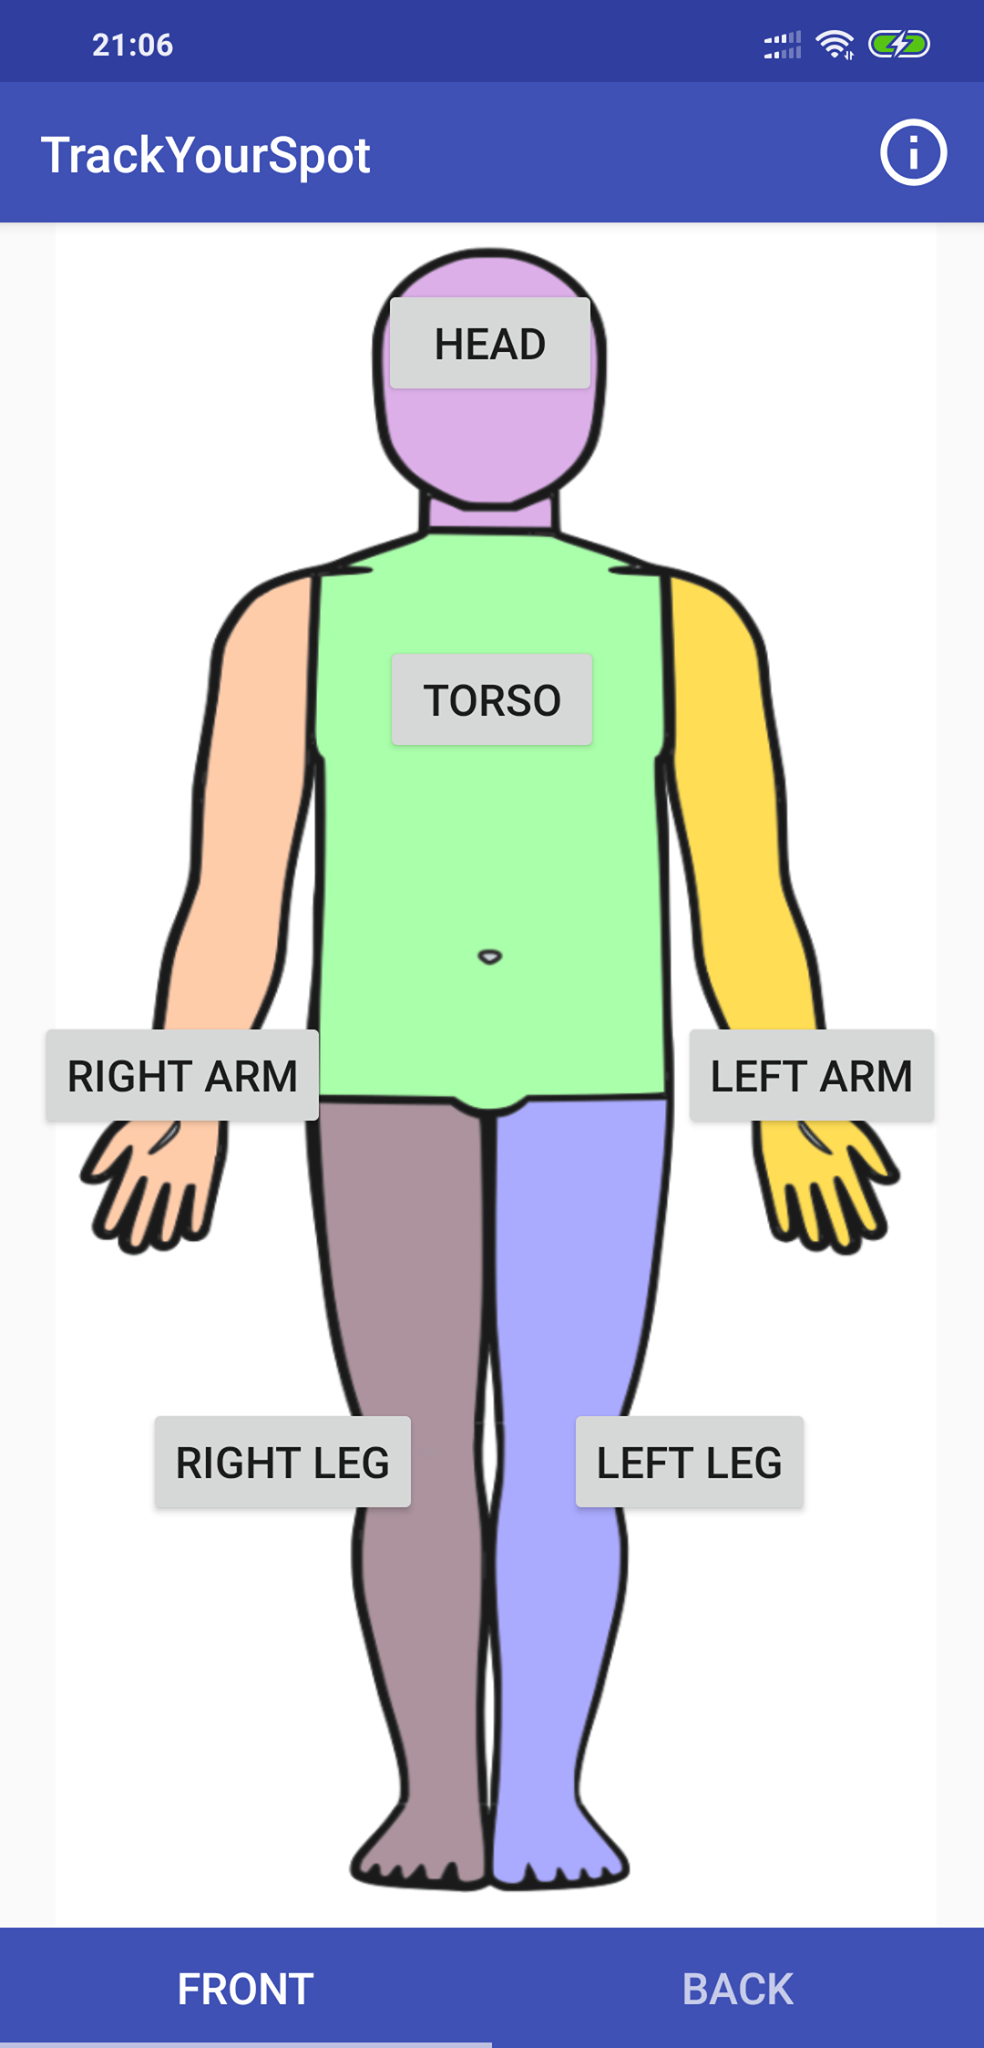
\includegraphics[height=10cm]{figures/frontbodybuttons.png}
        \caption{Front Body Screen}
    \end{subfigure}%
    ~
    \begin{subfigure}[t]{0.5\textwidth}
        \centering
        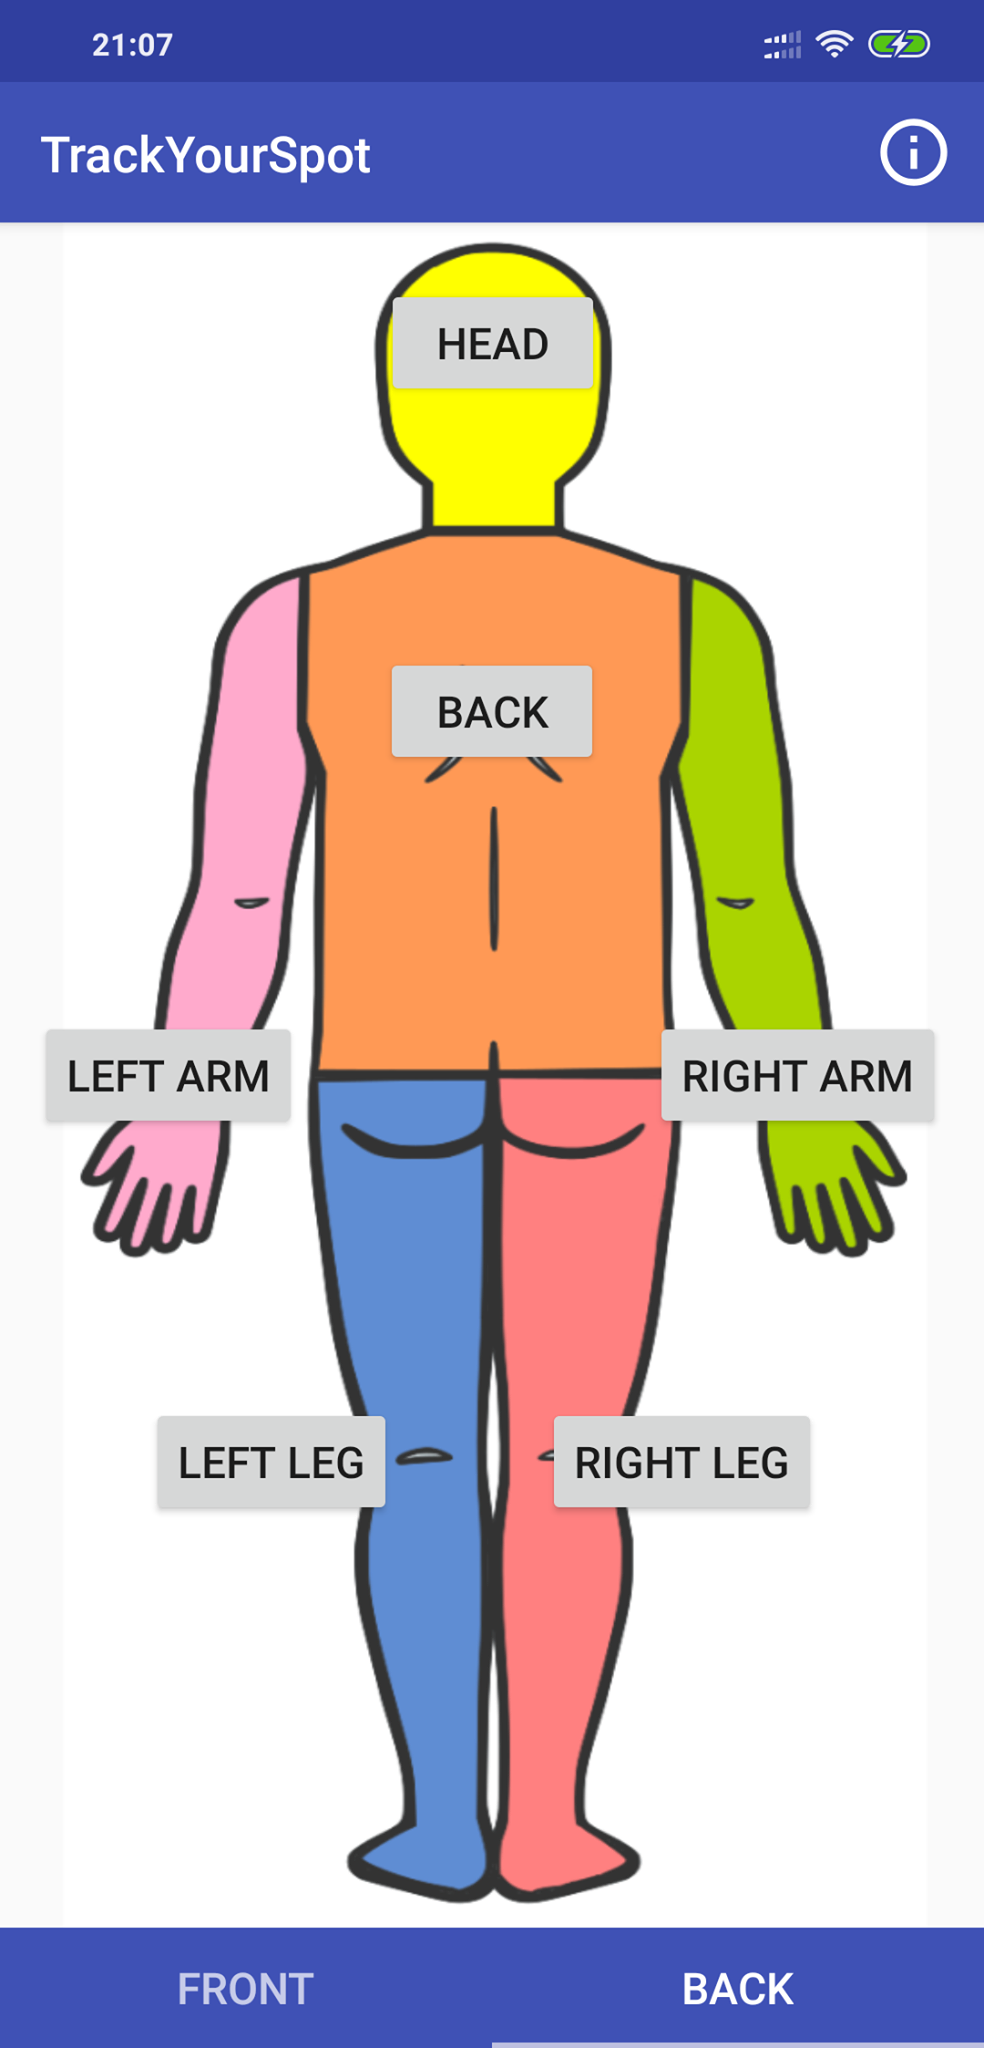
\includegraphics[height=10cm]{figures/backbodybuttons.png}
        \caption{Back Body Screen}
    \end{subfigure}
    \caption{App homepage body screen}
    \label{fig:bodyfinalscreen}
\end{figure*}

\clearpage
\begin{figure*}[t!]
    \centering
    \begin{subfigure}[t]{0.5\textwidth}
        \centering
        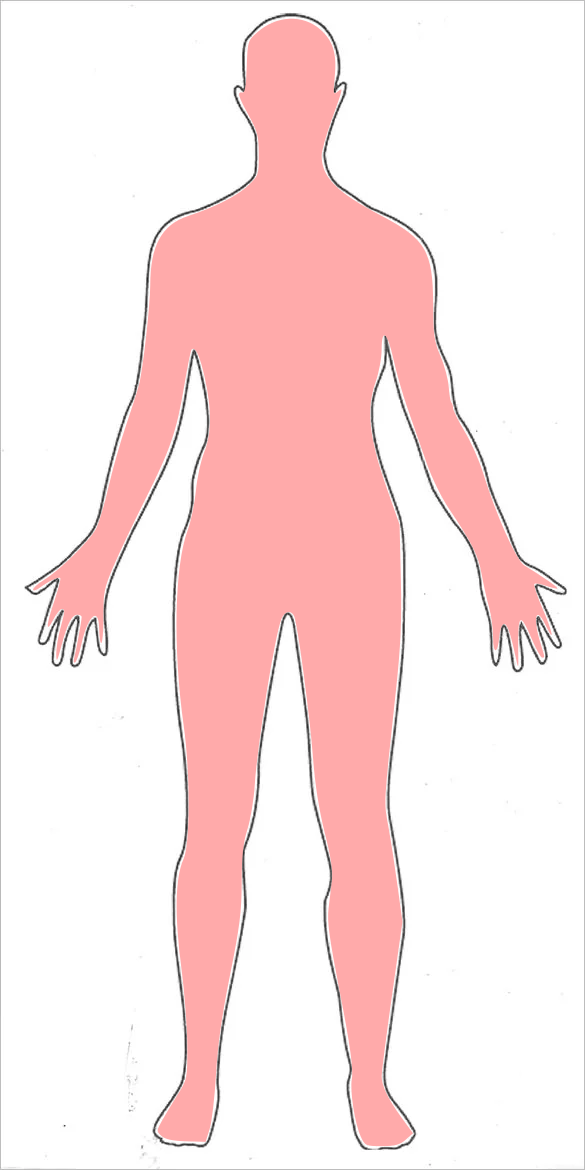
\includegraphics[height=10cm]{figures/bodydesign1front.png}
    \end{subfigure}%
    ~
    \begin{subfigure}[t]{0.5\textwidth}
        \centering
        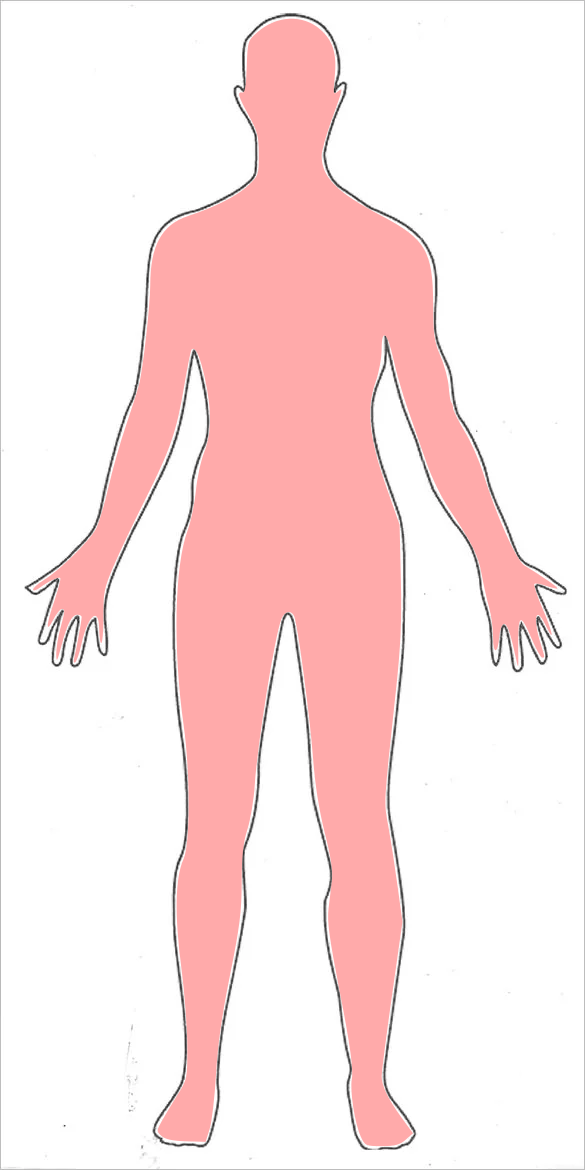
\includegraphics[height=10cm]{figures/bodydesign1front.png}
    \end{subfigure}
    \caption{Iteration 1 Body Designs}
    \label{fig:it1design}
\end{figure*}

\begin{figure*}[t!]
    \centering
    \begin{subfigure}[t]{0.5\textwidth}
        \centering
        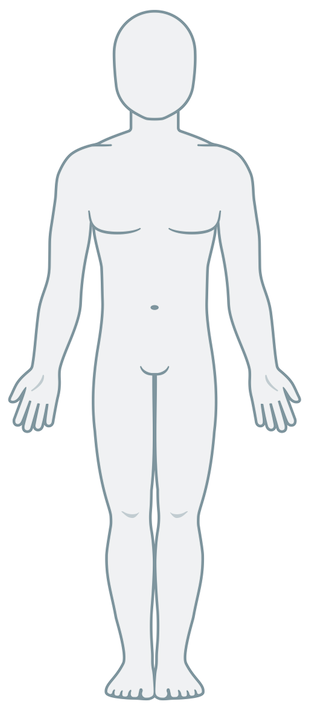
\includegraphics[height=10cm]{figures/bodydesign2front.png}
    \end{subfigure}%
    ~
    \begin{subfigure}[t]{0.5\textwidth}
        \centering
        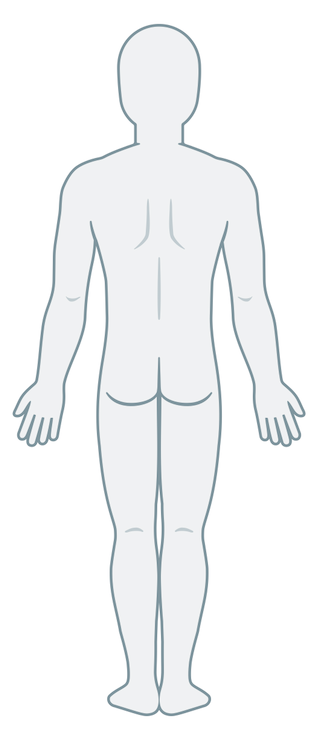
\includegraphics[height=10cm]{figures/bodydesign2back.png}
    \end{subfigure}
    \caption{Iteration 2 Body Designs}
    \label{fig:it2design}
\end{figure*}

\clearpage
\begin{figure*}[t!]
    \centering
    \begin{subfigure}[t]{0.5\textwidth}
        \centering
        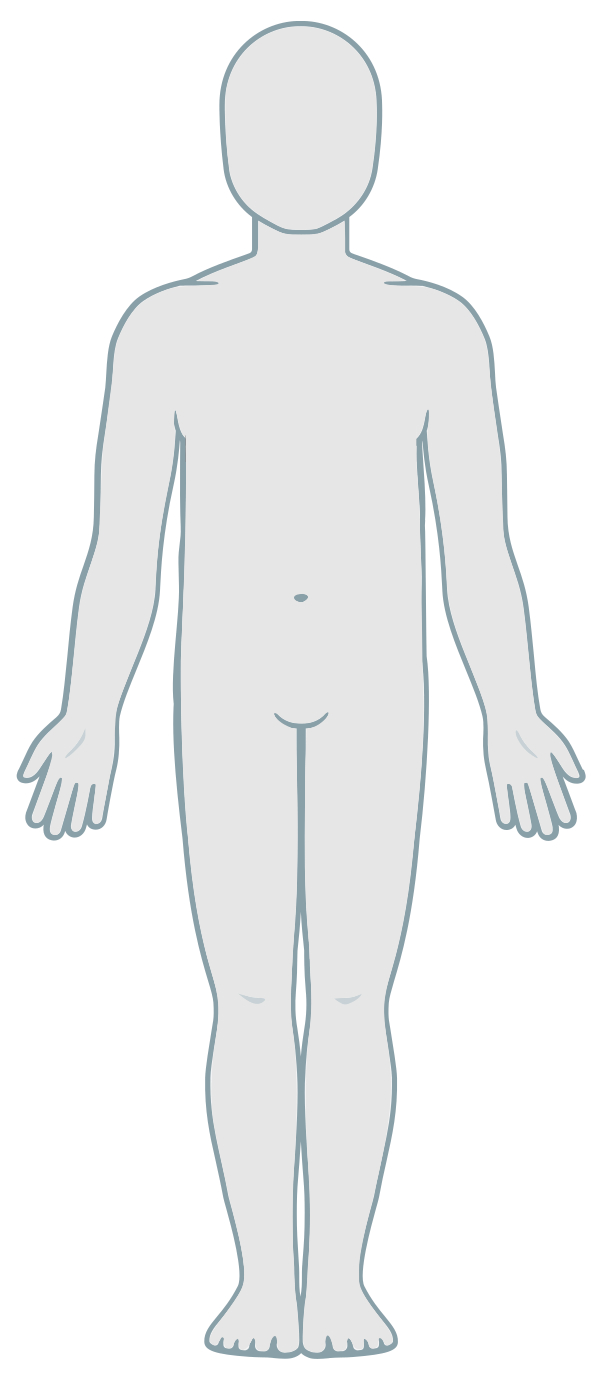
\includegraphics[height=10cm]{figures/bodydesign3front.jpg}
    \end{subfigure}%
    ~
    \begin{subfigure}[t]{0.5\textwidth}
        \centering
        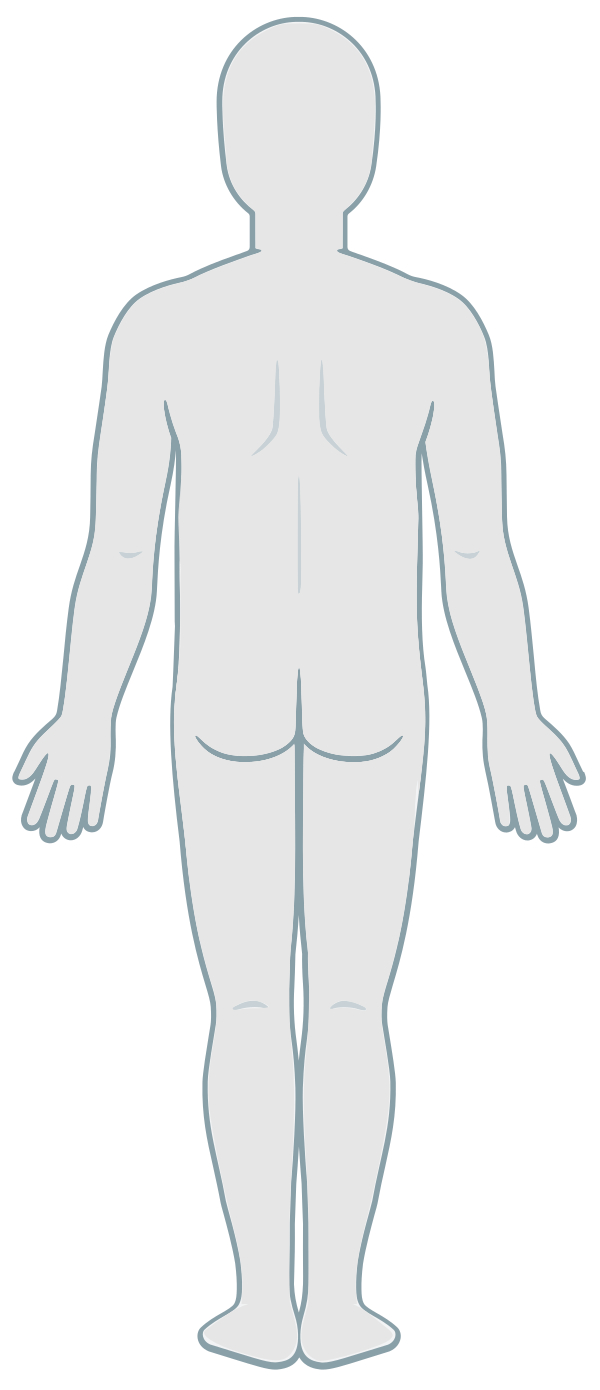
\includegraphics[height=10cm]{figures/bodydesign3back.jpg}
    \end{subfigure}
    \caption{Iteration 3 Body Designs}
    \label{fig:it3design}
\end{figure*}

\begin{figure*}[t!]
    \centering
    \begin{subfigure}[t]{0.5\textwidth}
        \centering
        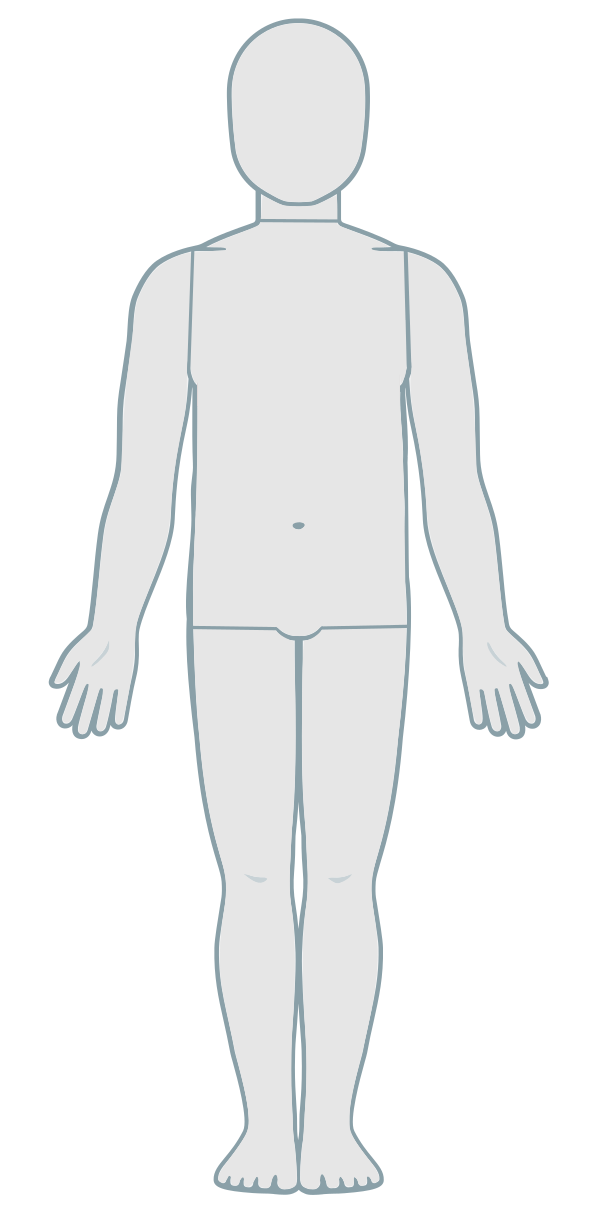
\includegraphics[height=10cm]{figures/bodydesign4front.png}
    \end{subfigure}%
    ~
    \begin{subfigure}[t]{0.5\textwidth}
        \centering
        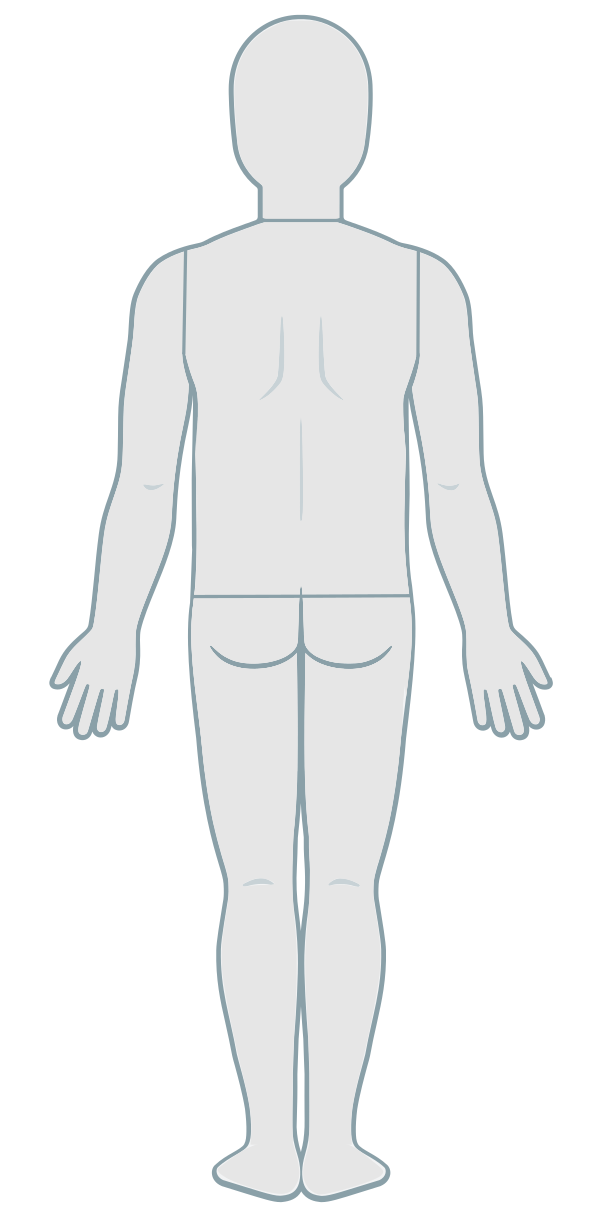
\includegraphics[height=10cm]{figures/bodydesign4back.png}
    \end{subfigure}
    \caption{Iteration 4 Body Designs}
    \label{fig:it4design}
\end{figure*}

\clearpage
\begin{figure*}[t!]
    \centering
    \begin{subfigure}[t]{0.5\textwidth}
        \centering
        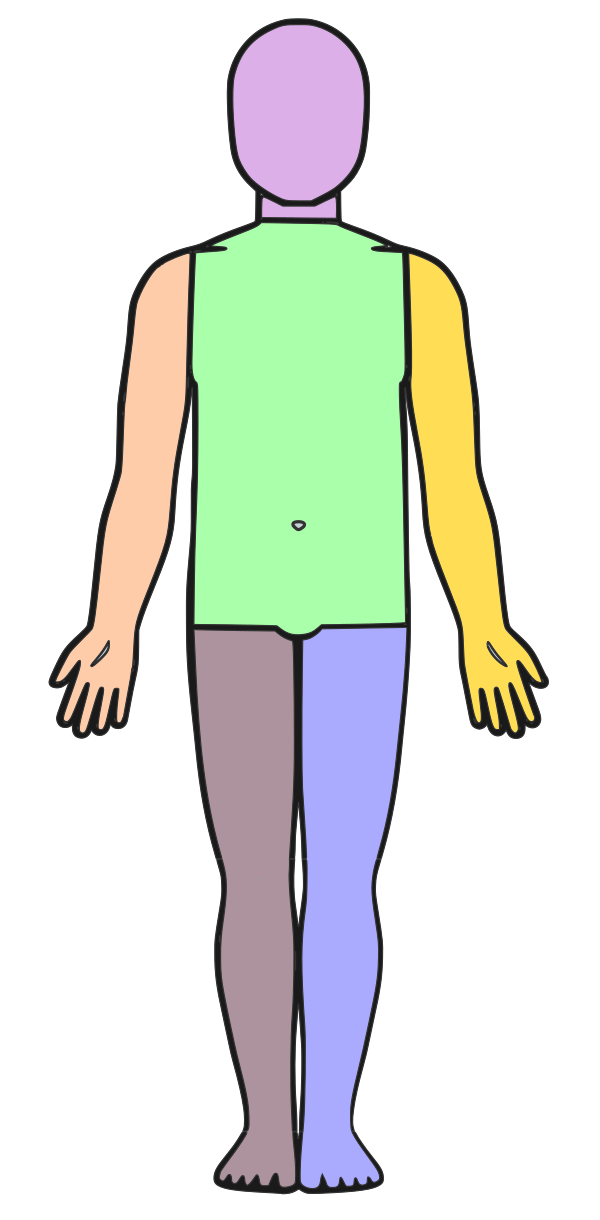
\includegraphics[height=10cm]{figures/bodydesign5front.png}
    \end{subfigure}%
    ~
    \begin{subfigure}[t]{0.5\textwidth}
        \centering
        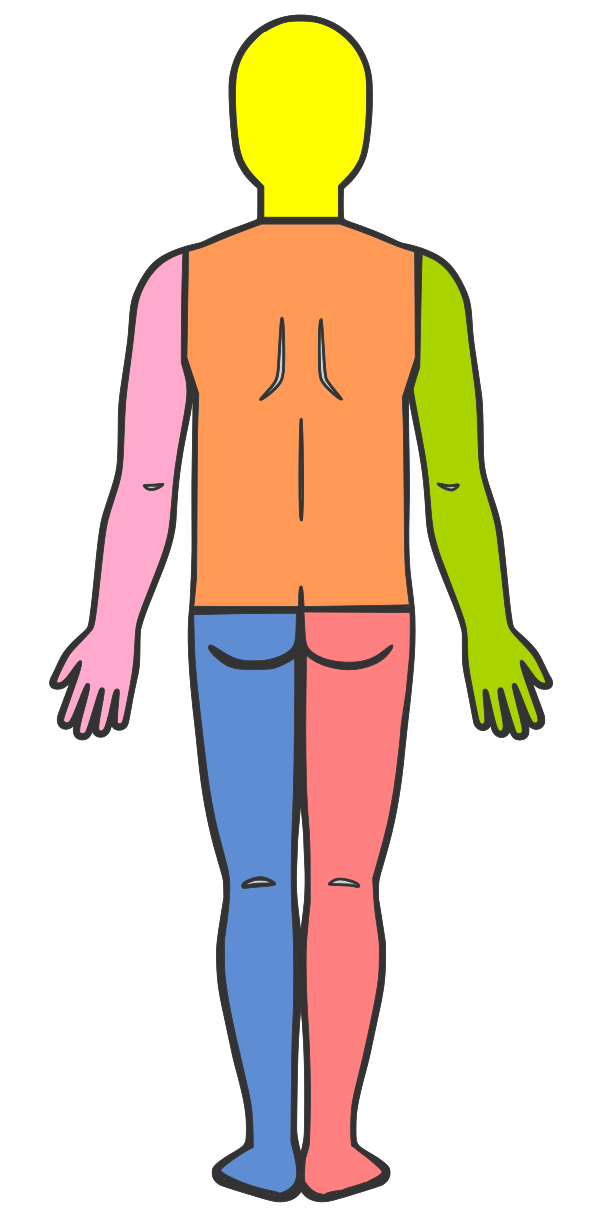
\includegraphics[height=10cm]{figures/bodydesign5back.png}
    \end{subfigure}
    \caption{Iteration 5 Body Designs}
    \label{fig:it15design}
\end{figure*}




\subsection{Information Screens} \label{sec:infoscreens}
As the title suggests, the information screens provide some background information on how to use the app in a safe manner. The screens in question are displayed in figure \ref{fig:infoscreens}. In order, the screens provide the following information concerning the following points:
\begin{enumerate}
    \item Danger of Skin Cancer
    \item Changes in Appeareance
    \item Preventing Skin Cancer
    \item Consulting a Doctor
\end{enumerate}

Ideally, the tutorial would also contain guidance on operating within the app, however, this would go against material design guidelines \cite{onboarding}, which suggest keeping tutorial screens short. A well-designed app user interface should require minimal tutorial help for the app to be used.

\clearpage
\begin{figure*}[t!]
    \centering
    \begin{subfigure}[t]{0.5\textwidth}
        \centering
        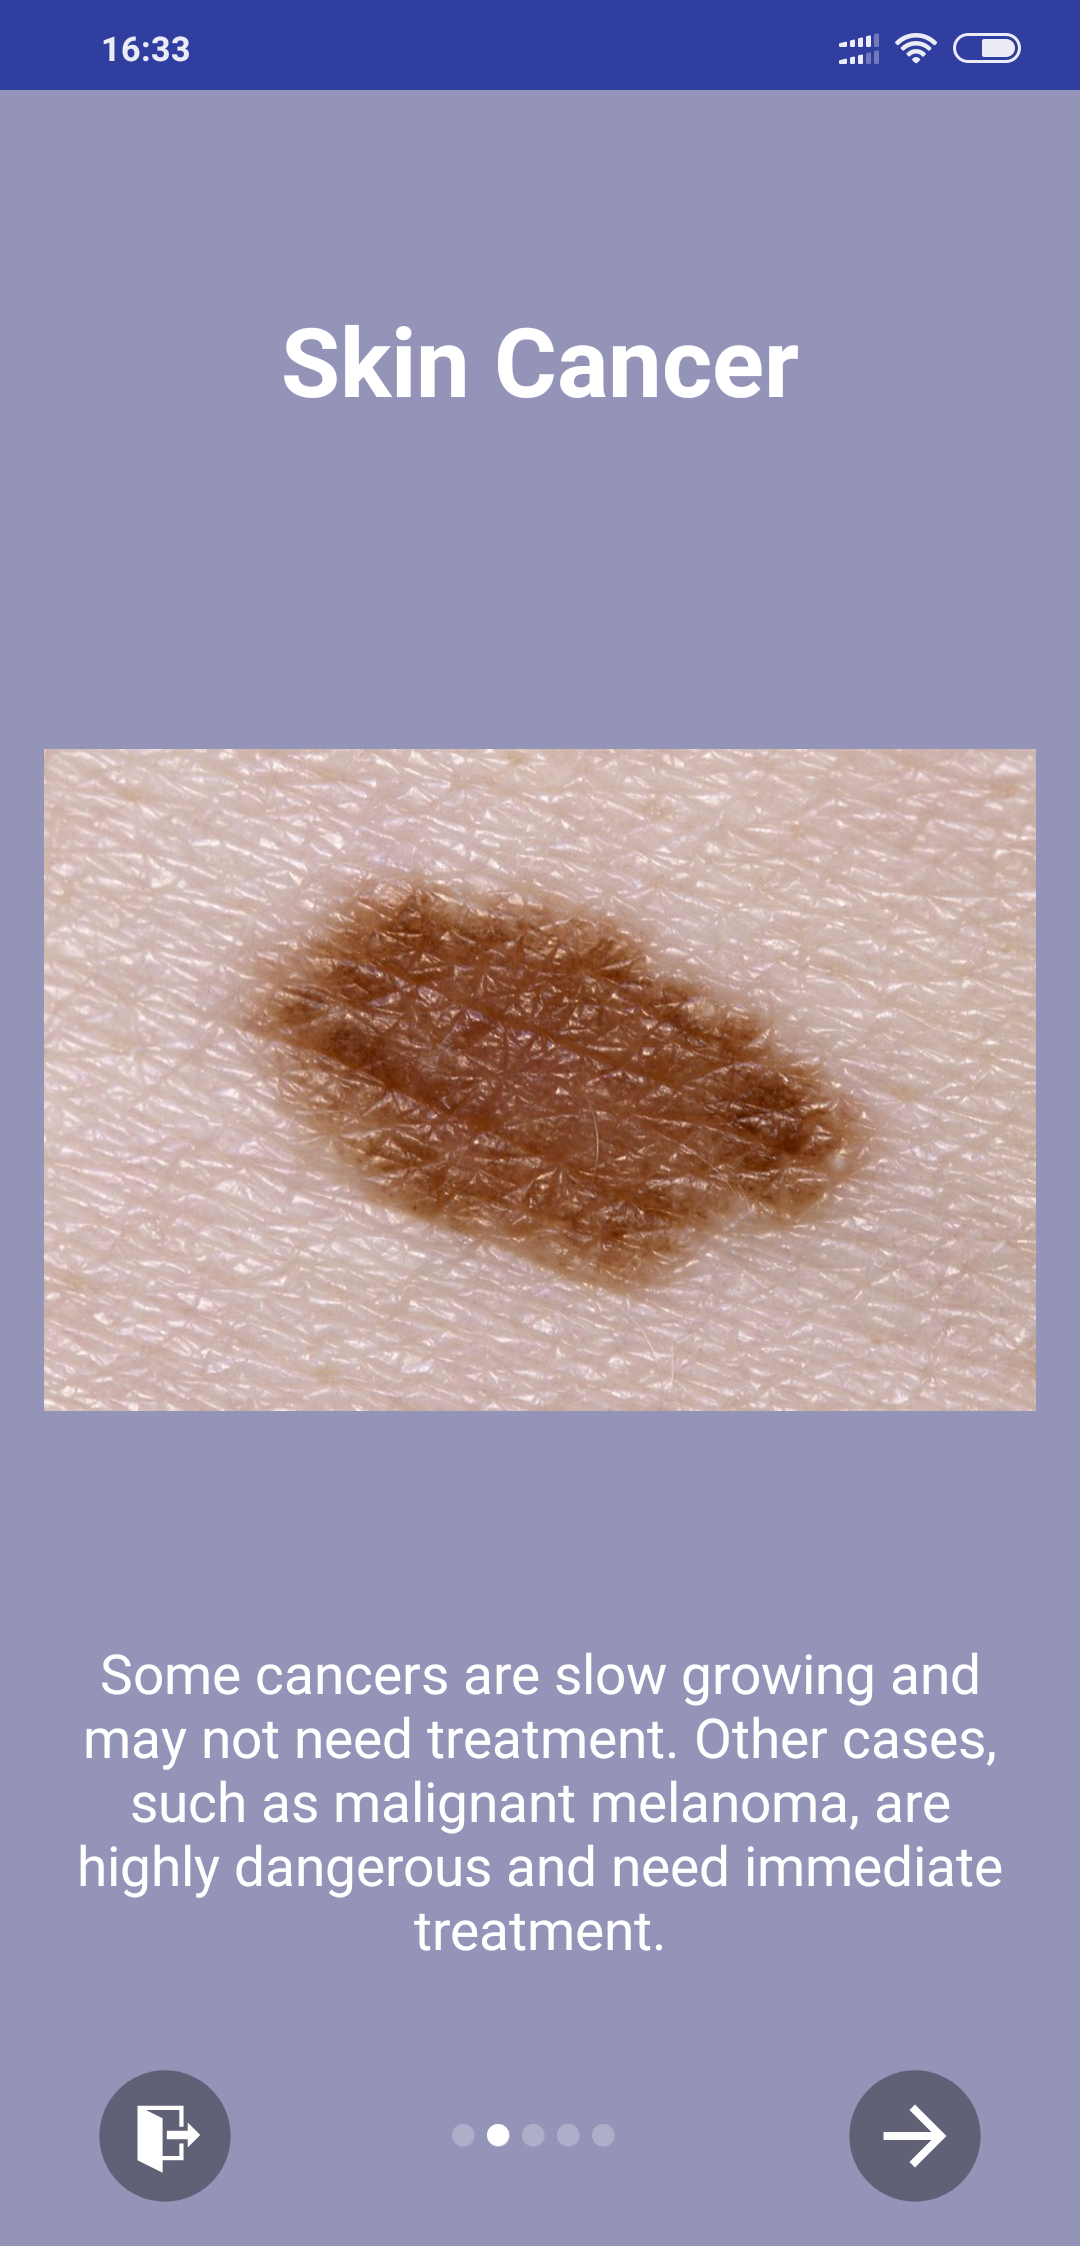
\includegraphics[height=10cm]{figures/info1_android.png}
        \caption{}
    \end{subfigure}%
    ~
    \begin{subfigure}[t]{0.5\textwidth}
        \centering
        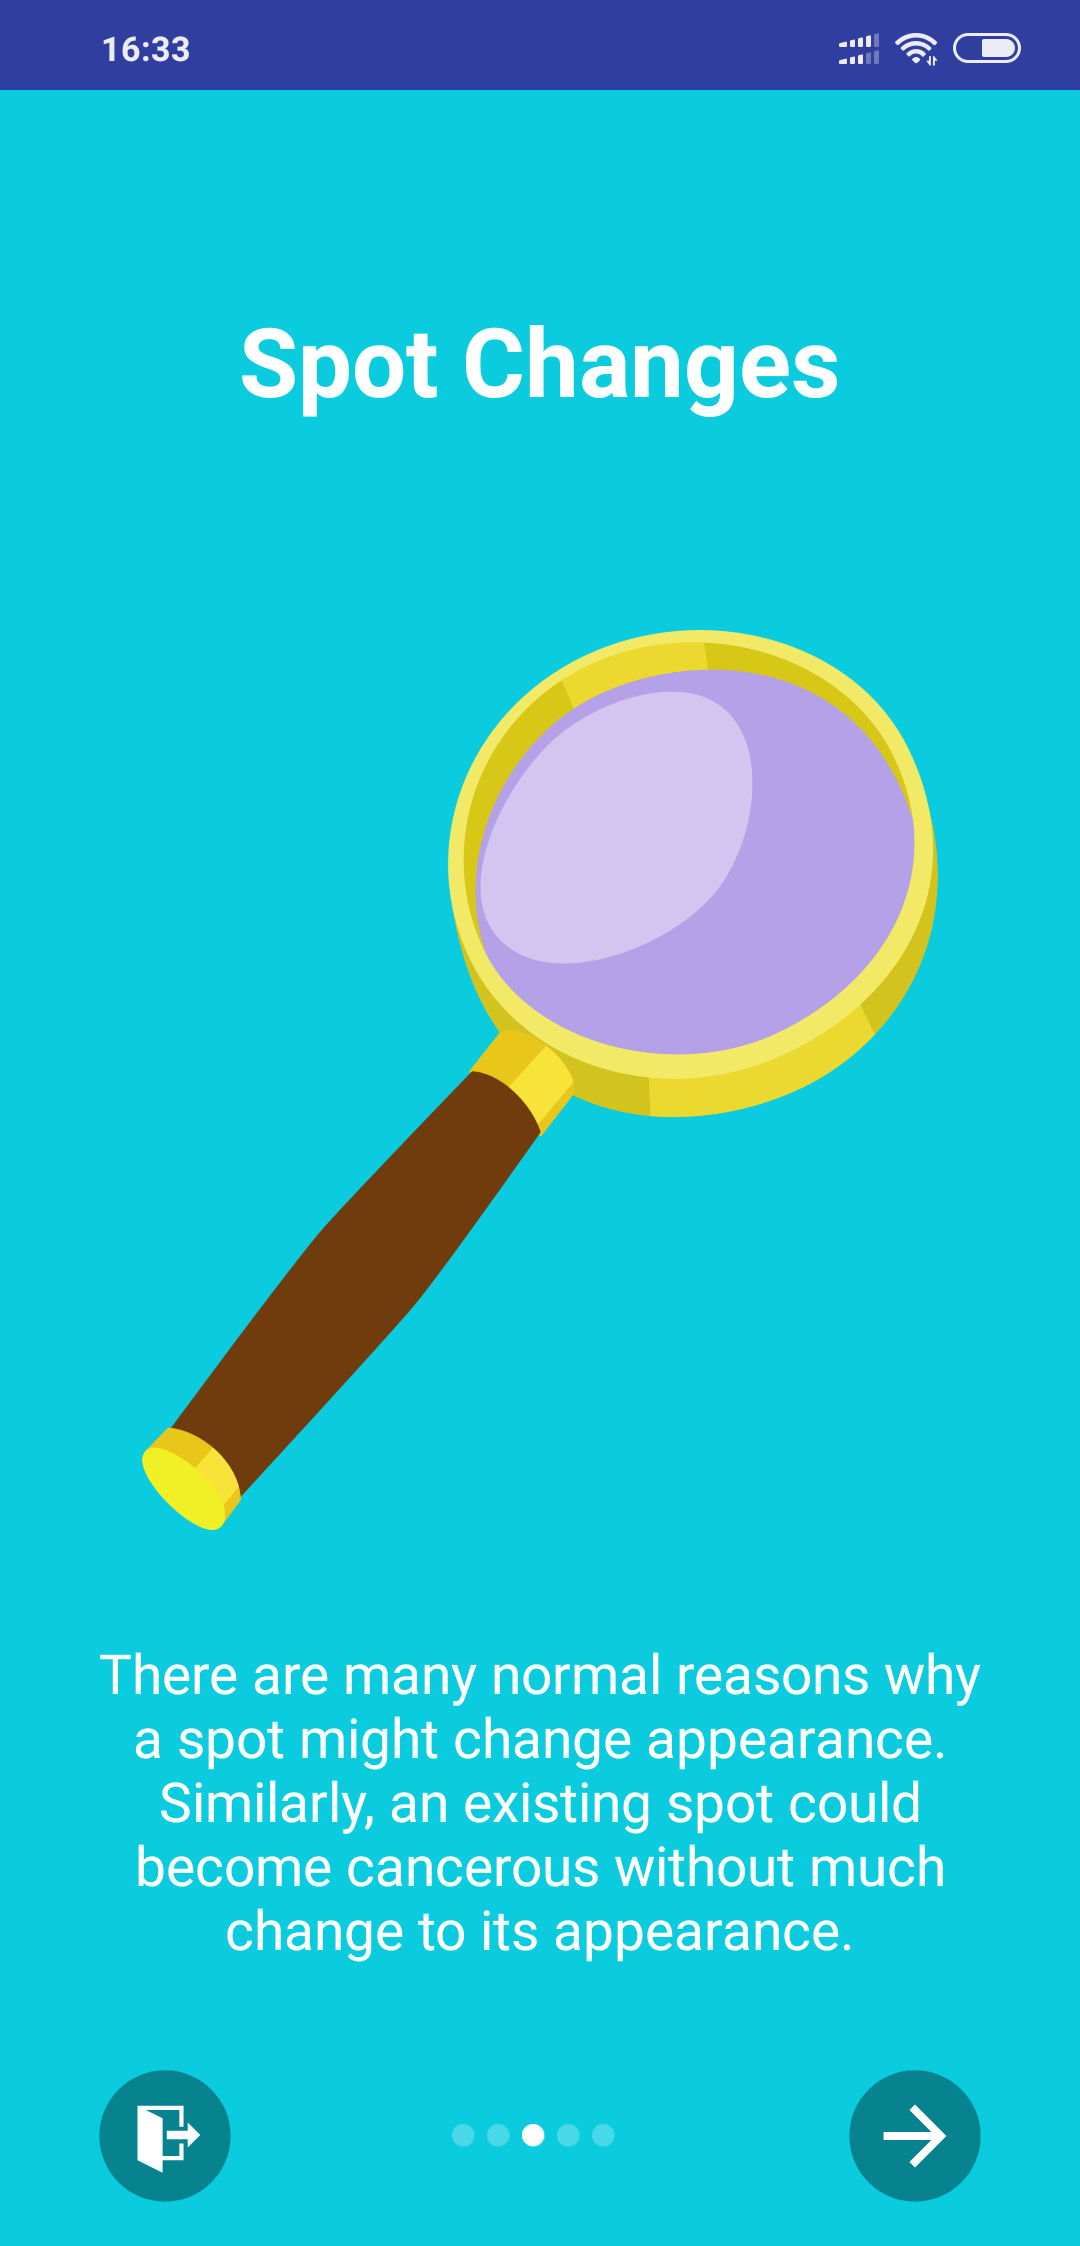
\includegraphics[height=10cm]{figures/info2_android.png}
        \caption{}
    \end{subfigure}
    \begin{subfigure}[t]{0.5\textwidth}
        \centering
        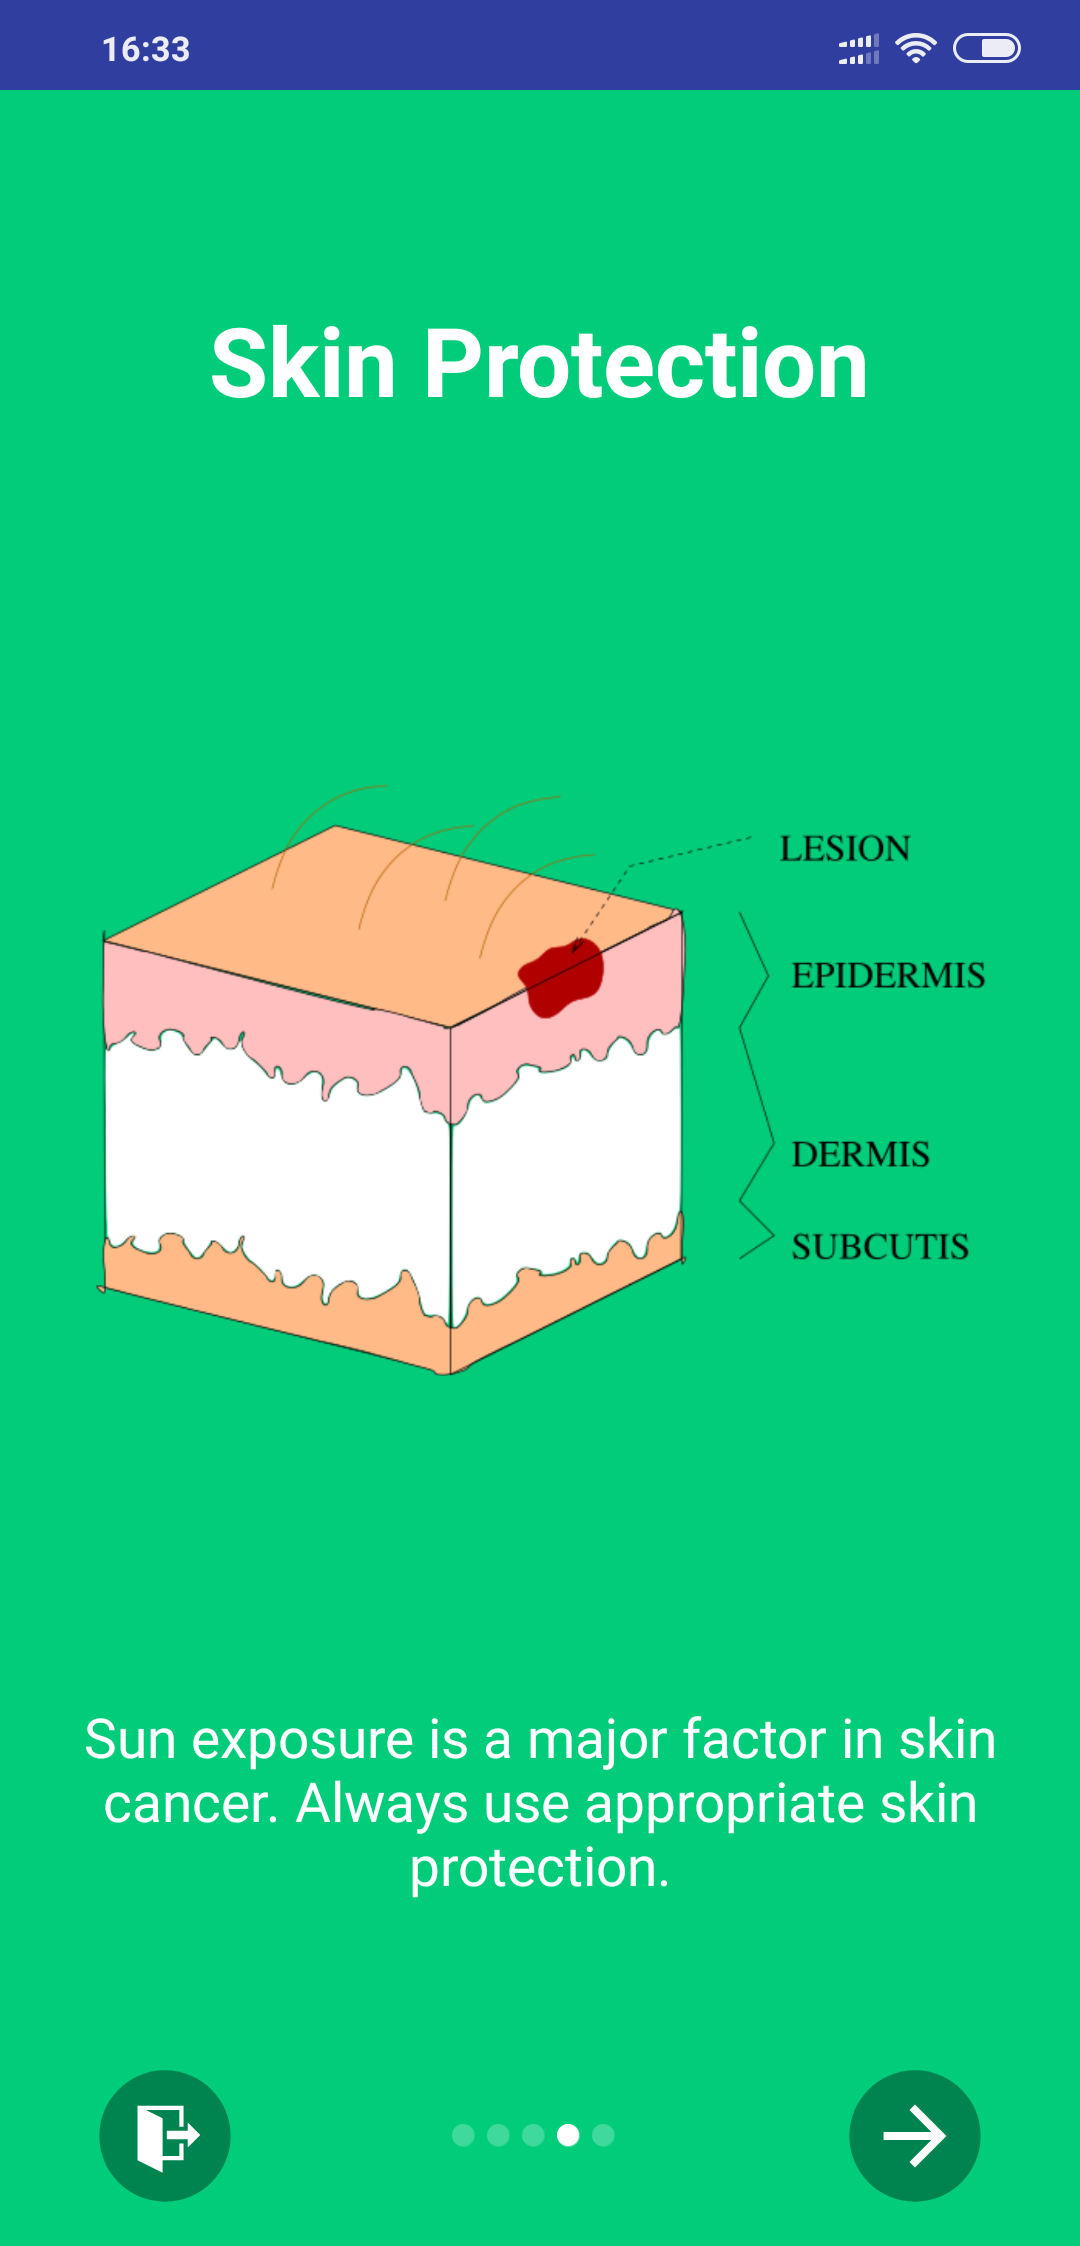
\includegraphics[height=10cm]{figures/info3_android.png}
        \caption{}
    \end{subfigure}%
    ~
    \begin{subfigure}[t]{0.5\textwidth}
        \centering
        
\includegraphics[height=10cm]{figures/info4_android.png}
        \caption{}
    \end{subfigure}
    \caption{Providing background information to the user through Information Screens}
    \label{fig:infoscreens}
\end{figure*}

\subsection{Old Spot Screen} \label{sec:oldspotscreen}
More accurately, this screen can be described as the screen displaying all previously added spots by the user in a selected body part. For example, if the user previously added the spots "Worrying Spot" and "Small normal spot" on their right arm, then these would be displayed in a list format on this screen. Each list item shows the spot name, a thumbnail of the spot, and the path of the spot in storage. From this screen, the user can:
\begin{itemize}
\item Add a new spot : By pressing the "+" button on the top right corner of the screen
\item Open a previously added spot: By selecting the spot from the displayed list of spots
\item Return to the body screen: By pressing the "$\leftarrow$" arrow button on the top left corner of the screen
\end{itemize}

\begin{figure*}[t!]
    \centering
    \begin{subfigure}[t]{0.5\textwidth}
        \centering
        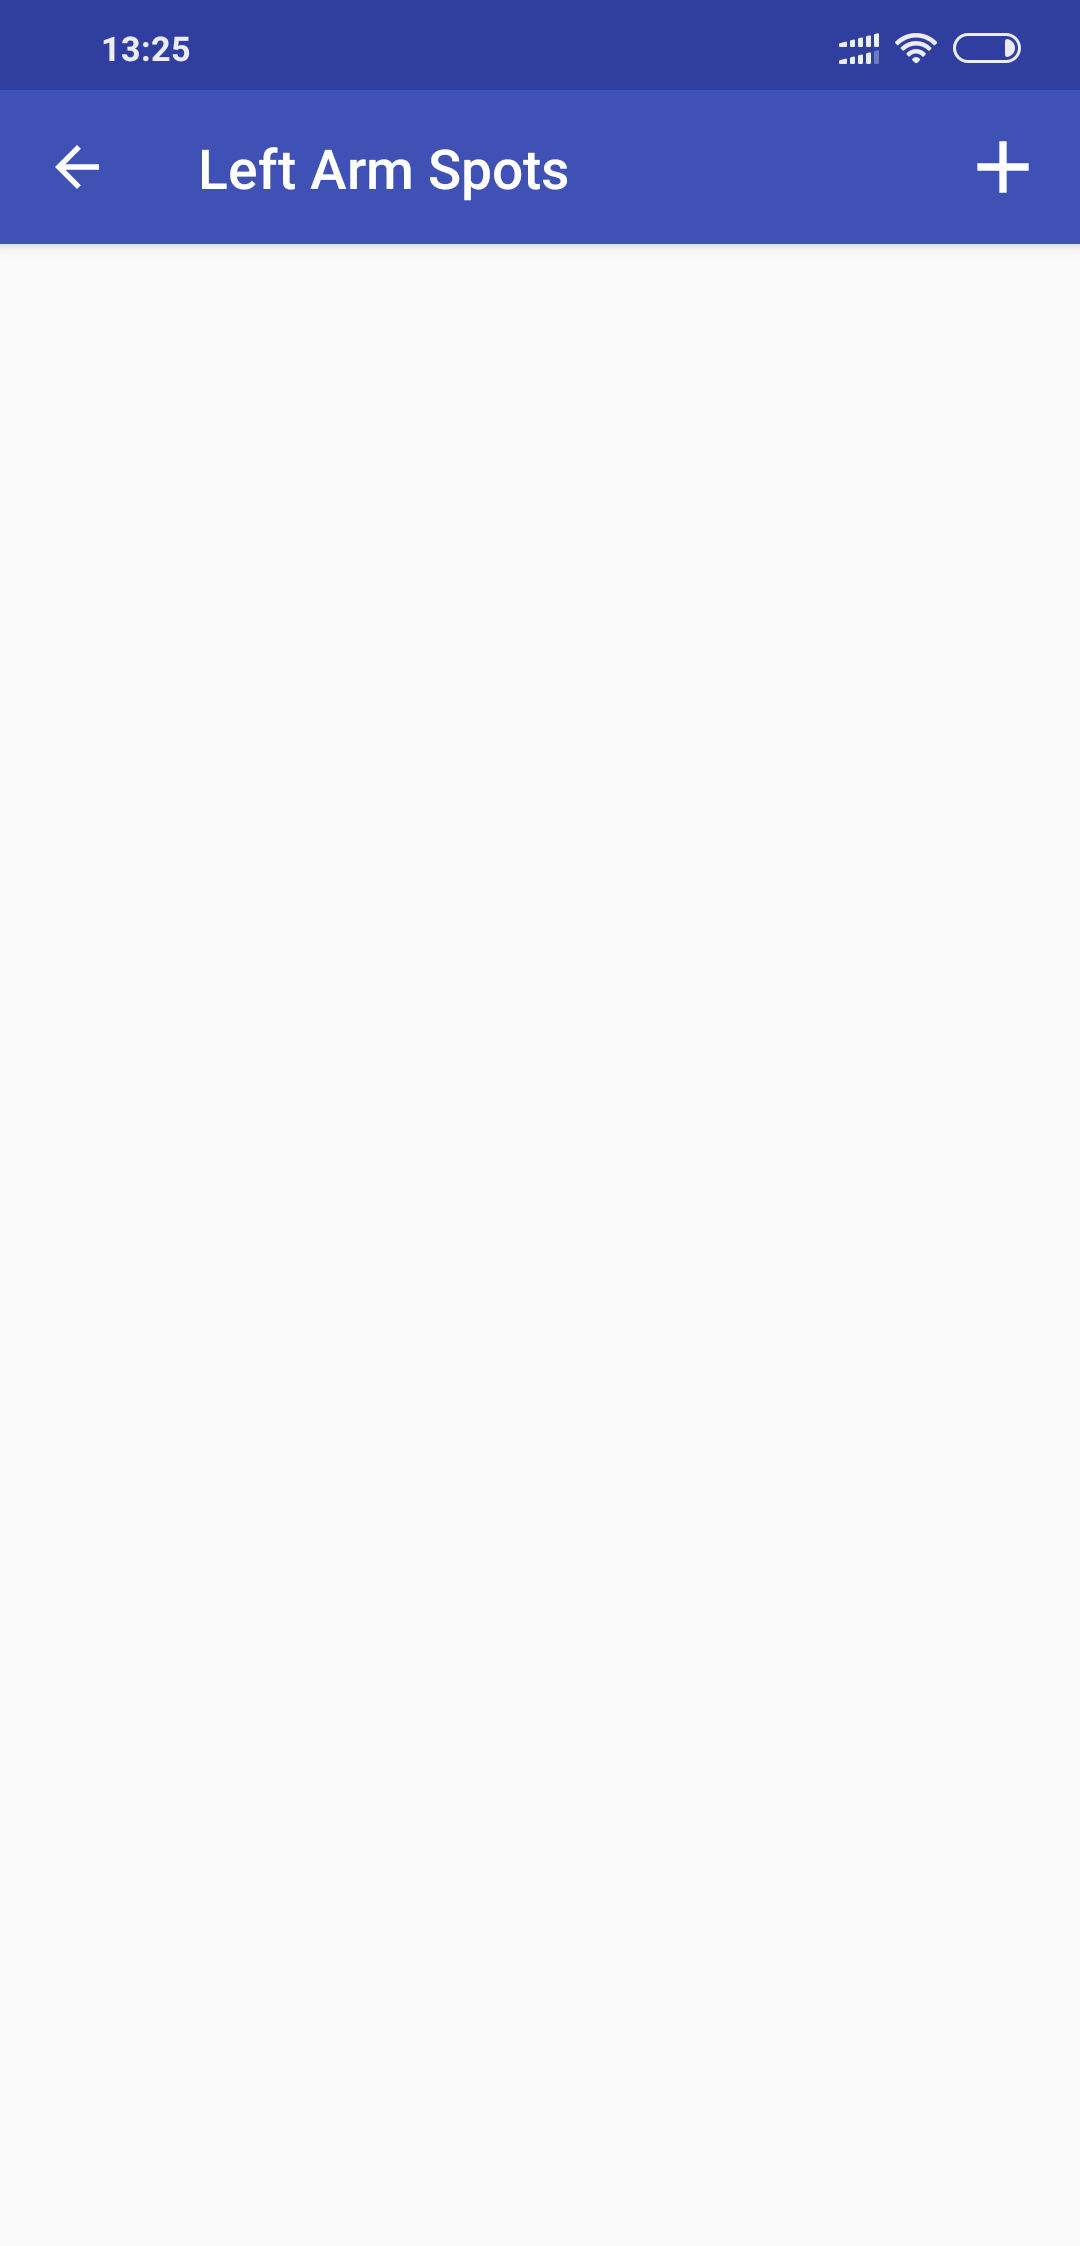
\includegraphics[height=10cm]{figures/spotlistempty_android.png}
        \caption{Empty Spot List}
    \end{subfigure}%
    ~
    \begin{subfigure}[t]{0.5\textwidth}
        \centering
        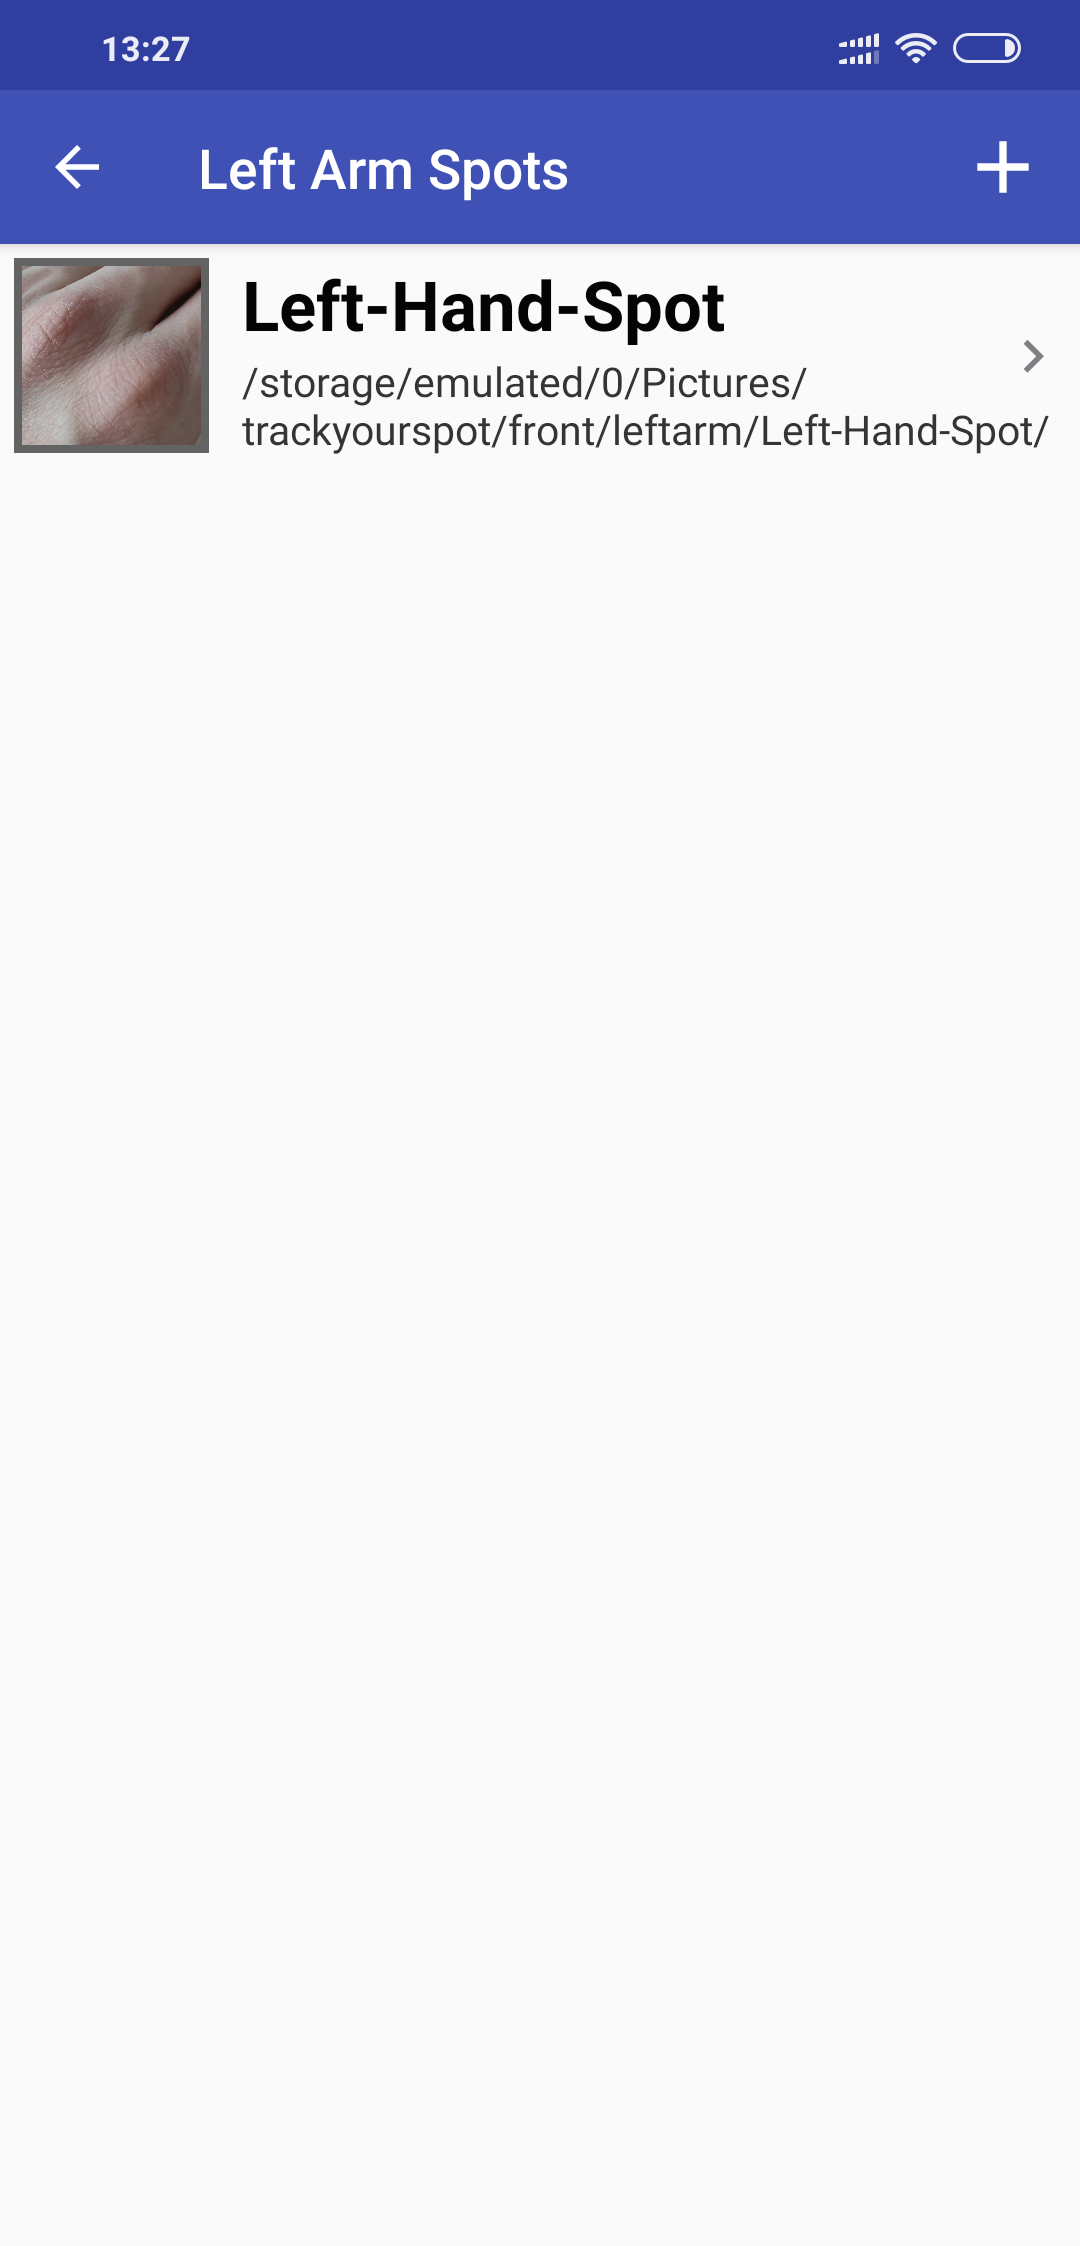
\includegraphics[height=10cm]{figures/spotlist_android.png}
        \caption{Left arm spot list after adding a spot}
    \end{subfigure}
    \caption{Old Spot Screen for the Left Arm}
\end{figure*}

\subsection{Camera and Cropping Screen}
These successive screens are displayed on two occasions: When a user elects to add a new spot, and when the user adds a new image to an old spot (spot update). This allows users to take a photo of a spot (Figure \ref{fig:cameraandcrop}), zoom in to a close up distance, and crop the image to a squared 1:1 aspect ratio. This ensures consistency across all images, so that all photos are of similar characteristics for easy comparison. The camera screen is provided by each user's default camera app, while the cropping screen is implemented through the uCrop Android Library \cite{yalantis_2019}. 

Using the Camera and uCrop API's means we are quite limited in customizing the appearance and design of these screens. The alternative would involve creating custom Activities and Screen layouts. However, this would require a very large amount of effort for a relatively low reward. Benefits would include drawing a "mask" or "frame" around the camera, so that the user knows how to better position the spot in the photo or cropping. This would also require implementing back-end storage manipulating functions for both the camera and cropping activities. On the contrary, using the APIs already provides a very flexible and user friendly UI, hence the decision was made to use these. 

Once the camera is open, the user can repeatedly take photos until they are happy with the image. This is indicated through the "\checkmark" or "x" symbols. Subsequently, the cropping activity opens the image. The cropping screen allows zooming in and rotating the image, both operated by a slider at the bottom of the screen. Once again, the user can proceed to save the photo with the "\checkmark" button, or cancel the action through the "x" button. This returns the app to the old spot or spot image list screens.

\begin{figure*}[t!]
    \centering
    \begin{subfigure}[t]{0.5\textwidth}
        \centering
        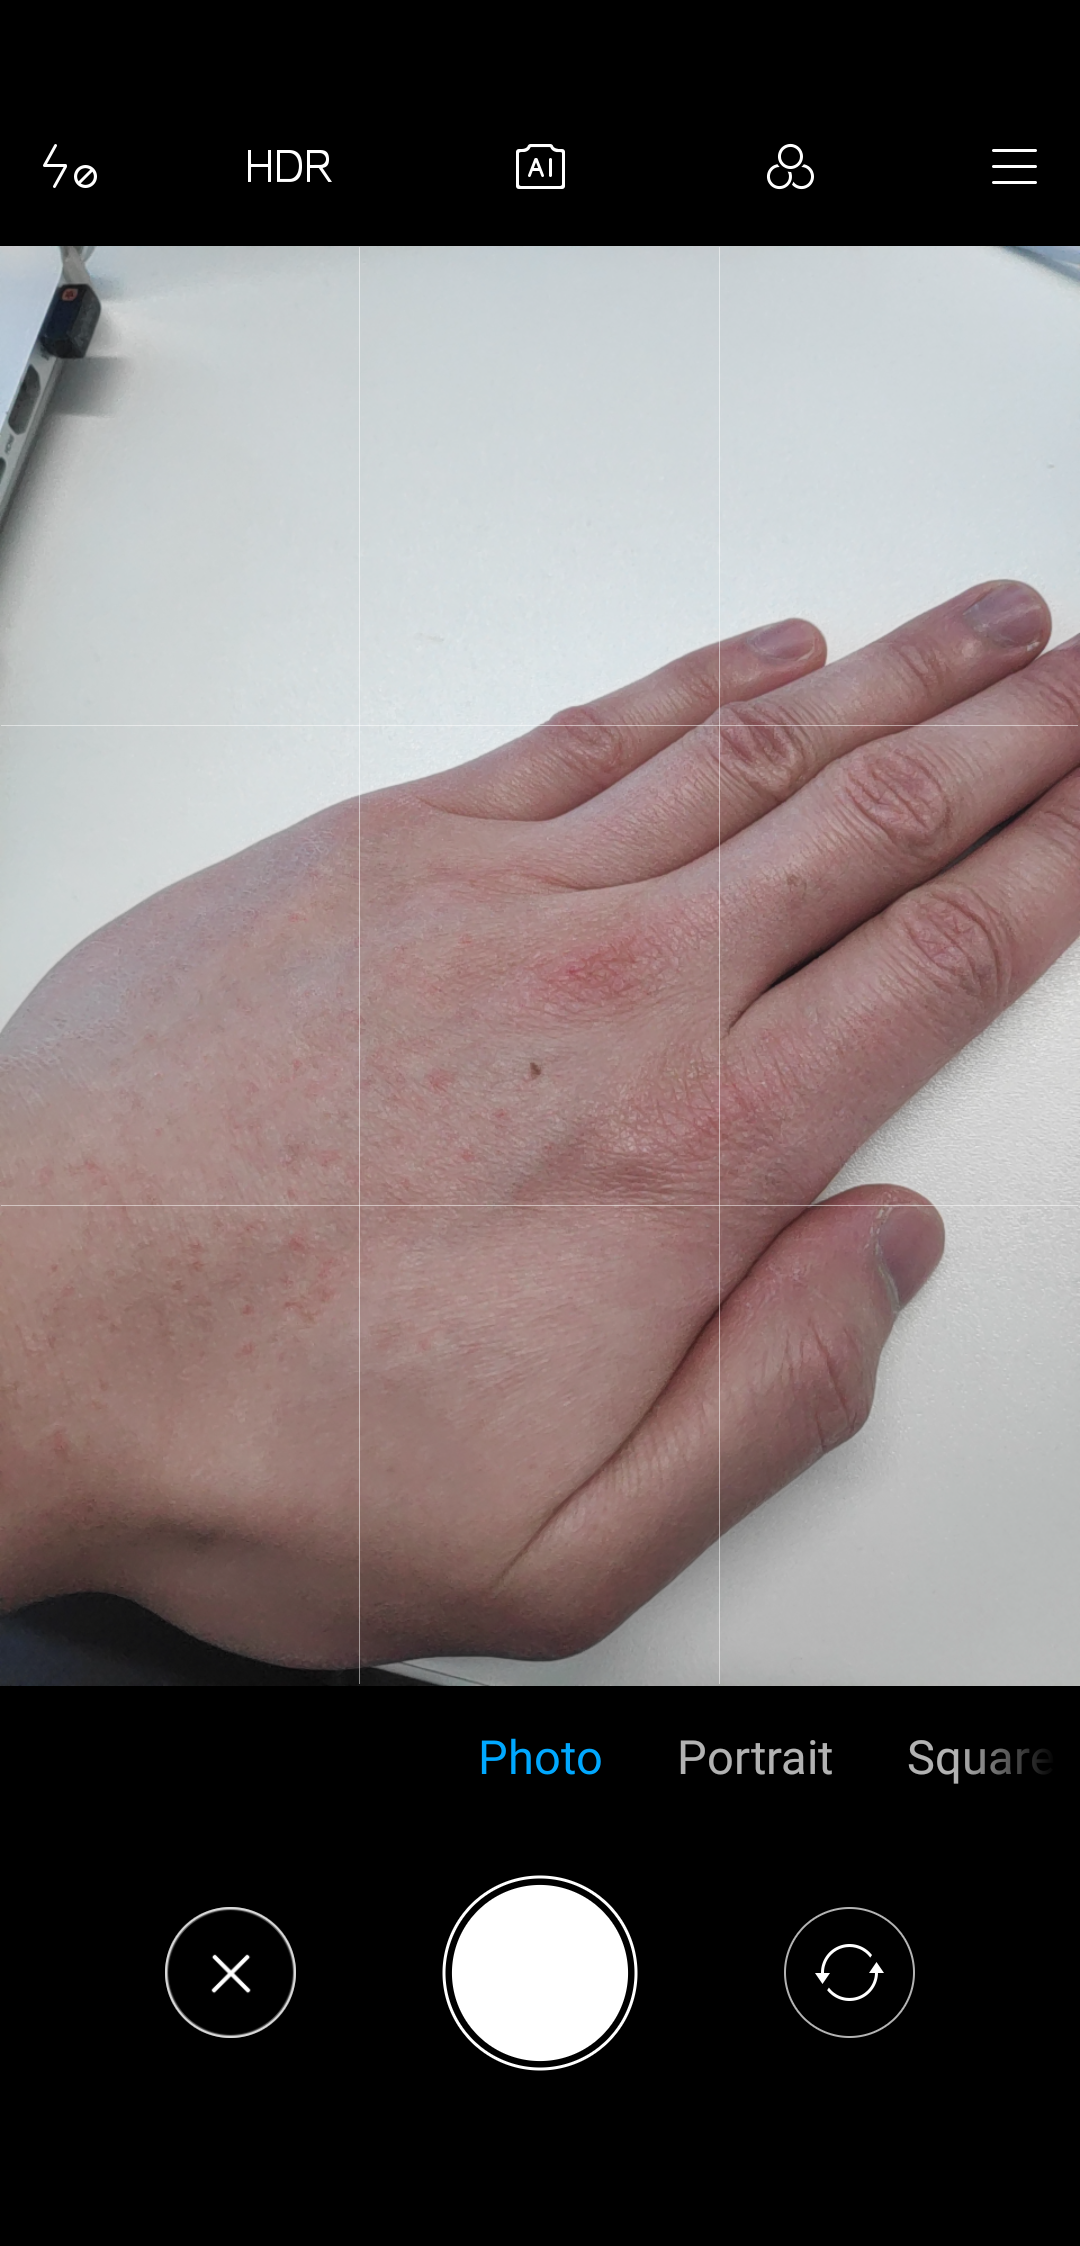
\includegraphics[height=10cm]{figures/camera1.png}
        \caption{Camera Screen after selecting to add a new spot}
    \end{subfigure}%
    ~
    \begin{subfigure}[t]{0.5\textwidth}
        \centering
        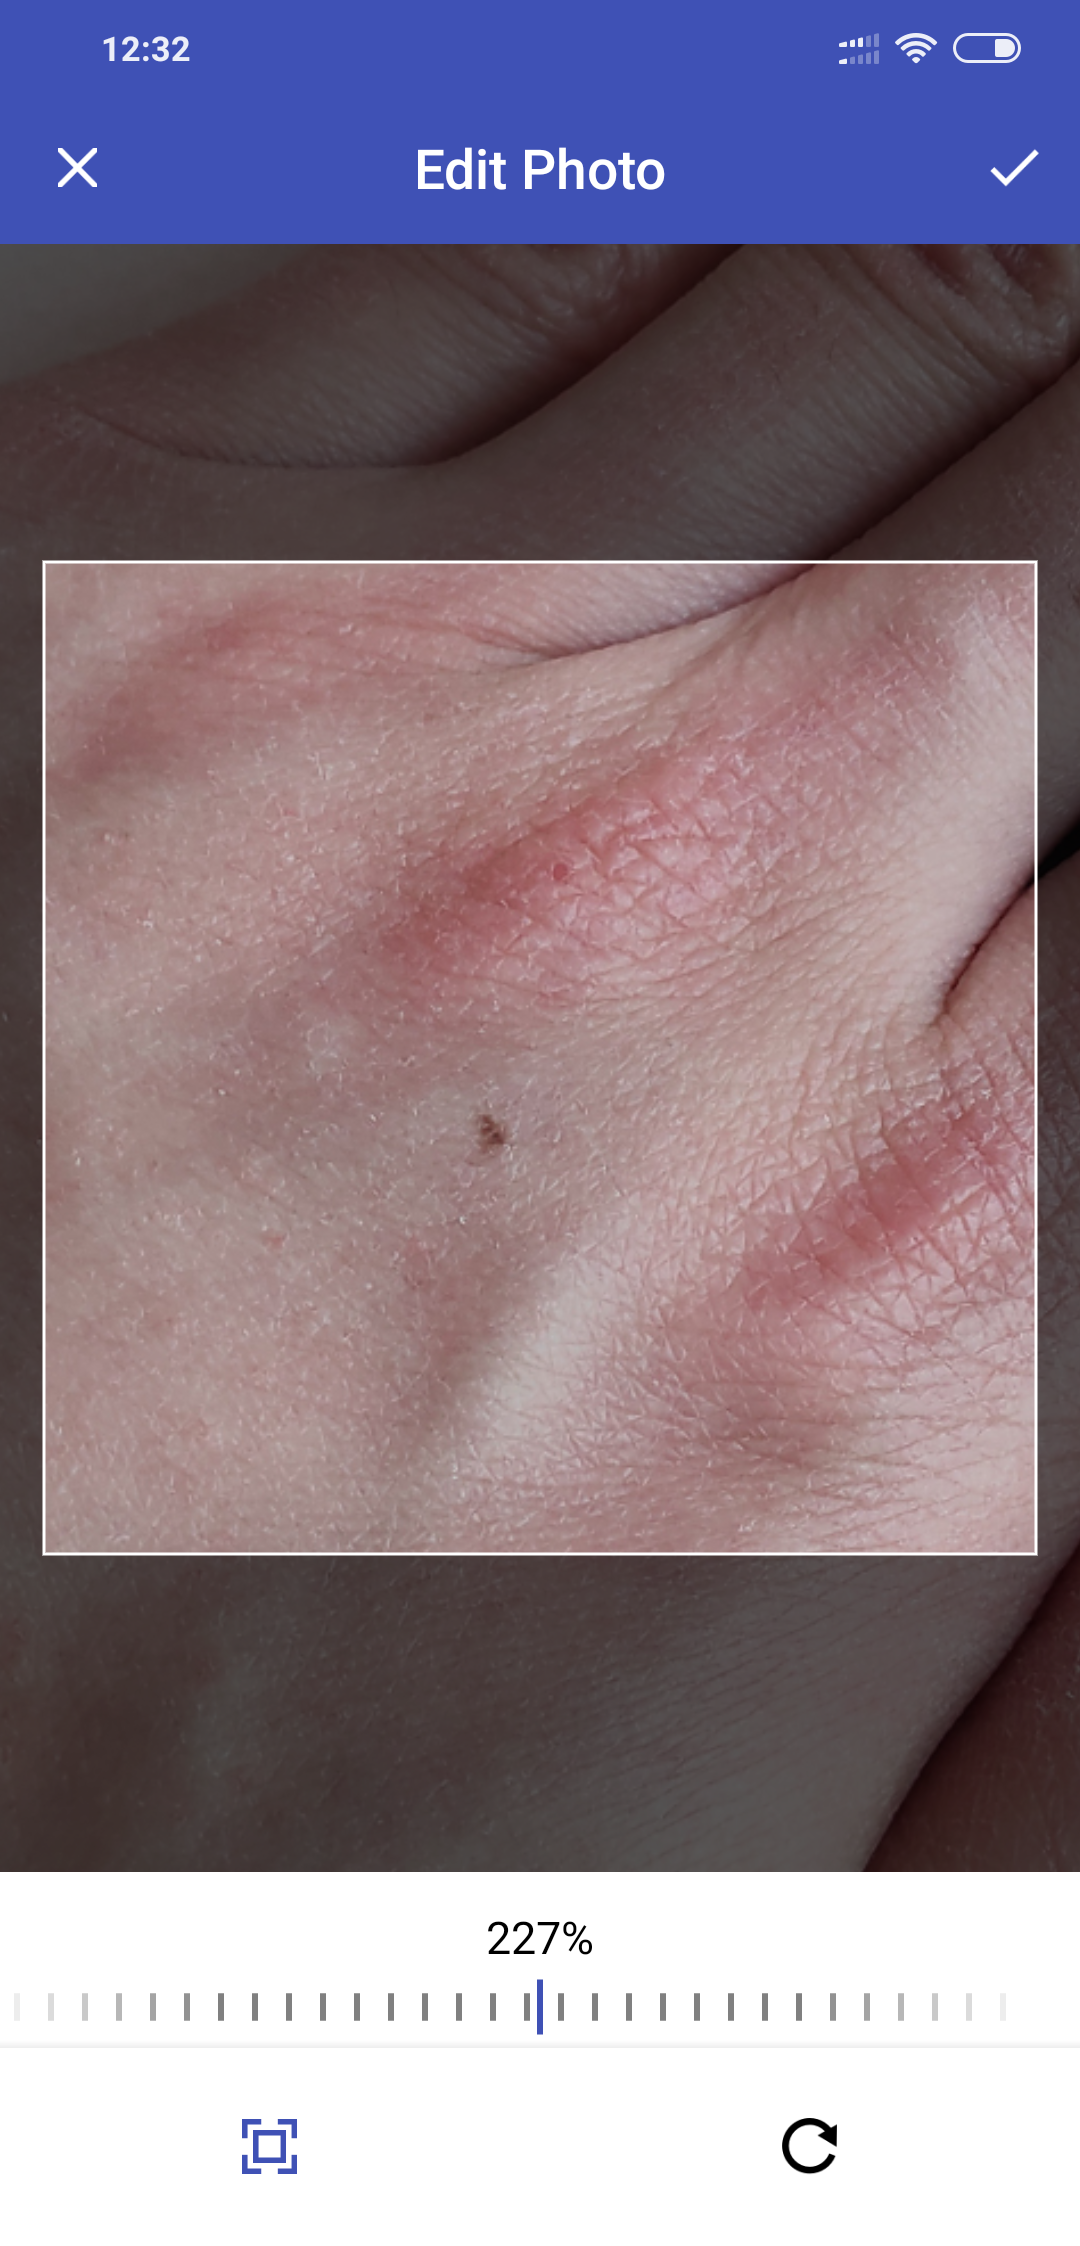
\includegraphics[height=10cm]{figures/crop1.png}
        \caption{Cropping Screen after zooming in to the chosen spot}
    \end{subfigure}
    \caption{Camera and Cropping Screens}
    \label{fig:cameraandcrop}
\end{figure*}

\subsection{Spot Naming Screen}
This screen is used to give a name to a new spot, this name is useful to better identify a spot when adding newer images in the future. Figures \ref{subfig:oldaddspot} and \ref{subfig:oldaddspotkeyboard} show the very first initial design, later evolving into designs \ref{subfig:newaddspotkeyboard} and \ref{subfig:newaddspotnokeyboard} (Showing and hiding the keyboard respectively).

This screen contains a text input field to name the spot, a large preview of the photo that has just been taken, and two aligned buttons labelled "Cancel" and "Confirm". Clicking either button would take the user back to the SpotList screen. However, the confirm button would succesfully add the new spot to the list, while the cancel button deletes the image and returns to the previous spot list.

To justify the final design, the advantages and disadvantages of both designs can be compared. The initial design appears to be very basic, lacking an option to cancel the process of adding the spot. The design makes little use of screen size, leaving much of the display blank and keeping the image preview small in size. This could prove to be an issue with tiny spots or low quality images. The new design in Figures \ref{subfig:newaddspotkeyboard} and \ref{subfig:newaddspotnokeyboard} addresses these issues accordingly, providing a much larger, half-screen view of the image, allowing even very small spots to be clearly visible (assuming the image has been cropped sensibly). The text entry field now has its own container, separating more clearly the different components of the screen. Following official Android design guidelines for image positioning \cite{materialdesignimageplacement}, the image has been anchored to the top of the screen, with text right below it, this also makes the app more consistent with common image or social networking apps. Furthermore, the image and name container will always be visible even with the keyboard displayed. Lastly, a "Cancel" button gives the user flexibility to restart the spot adding process if they are unhappy with the image. This can also be done with the "$\leftarrow$" arrow button on the top left corner.
\clearpage
\begin{figure*}[t!]
    \centering
    \begin{subfigure}[t]{0.5\textwidth}
        \centering
        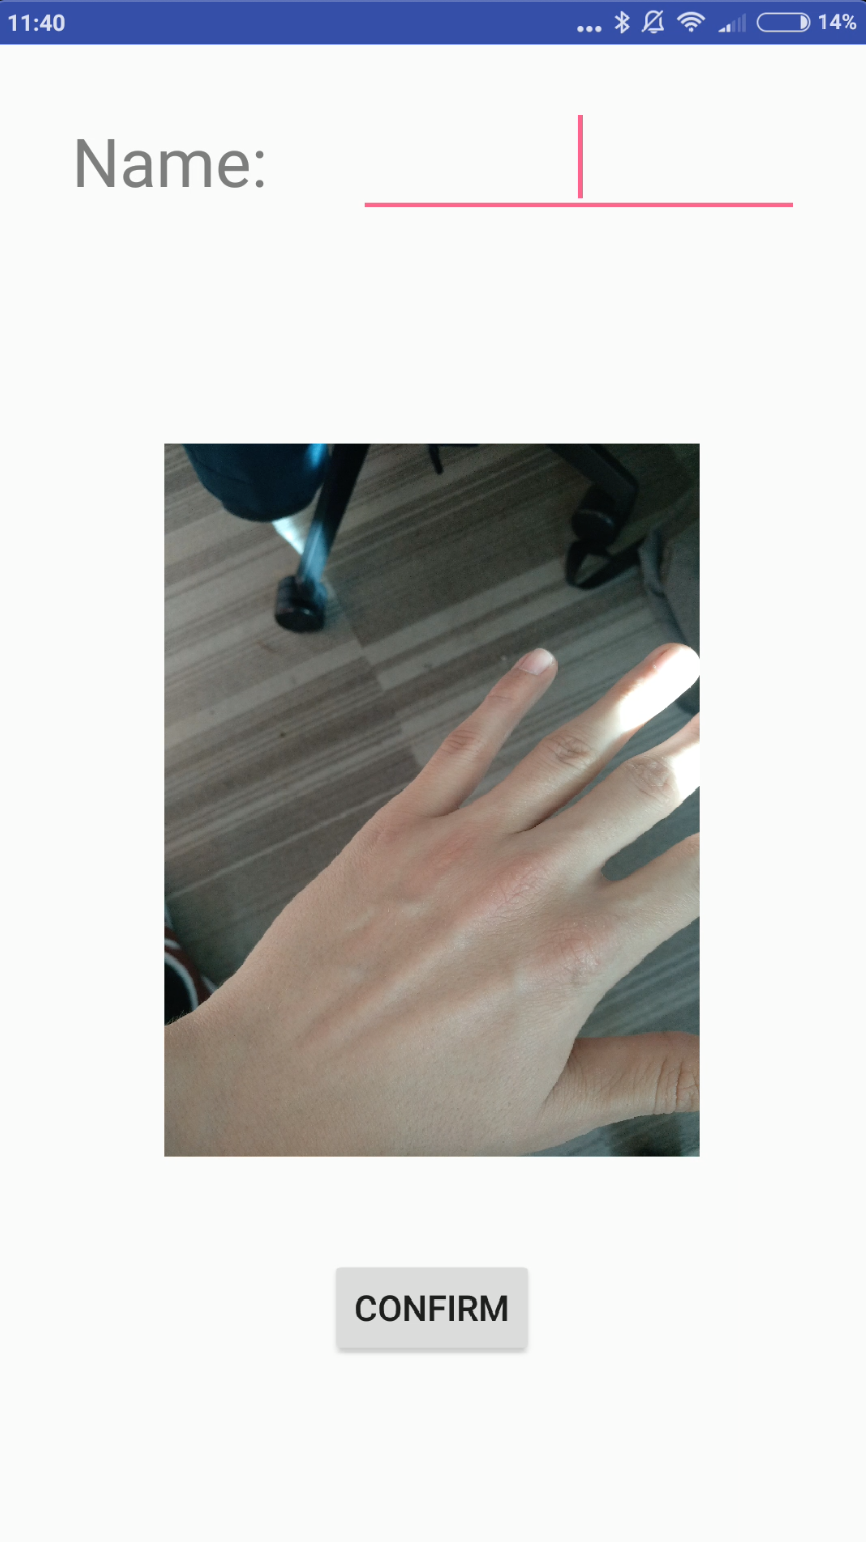
\includegraphics[height=10cm]{figures/addspot1.png}
        \caption{Initial AddSpot Activity screen}
        \label{subfig:oldaddspot}
    \end{subfigure}%
        ~
    \begin{subfigure}[t]{0.5\textwidth}
        \centering
        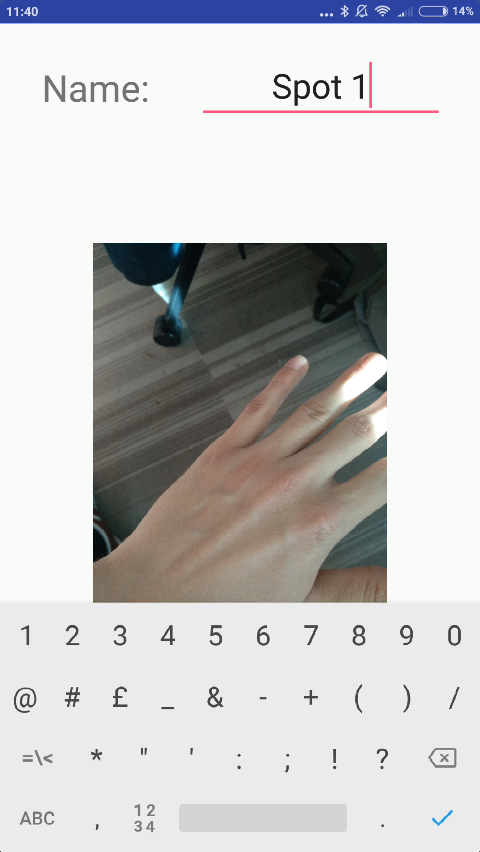
\includegraphics[height=10cm]{figures/oldaddspotkeyboard.png}
        \caption{Initial AddSpot Activity Screen showing the keyboard}
        \label{subfig:oldaddspotkeyboard}
    \end{subfigure}
    ~
    \begin{subfigure}[t]{0.5\textwidth}
        \centering
        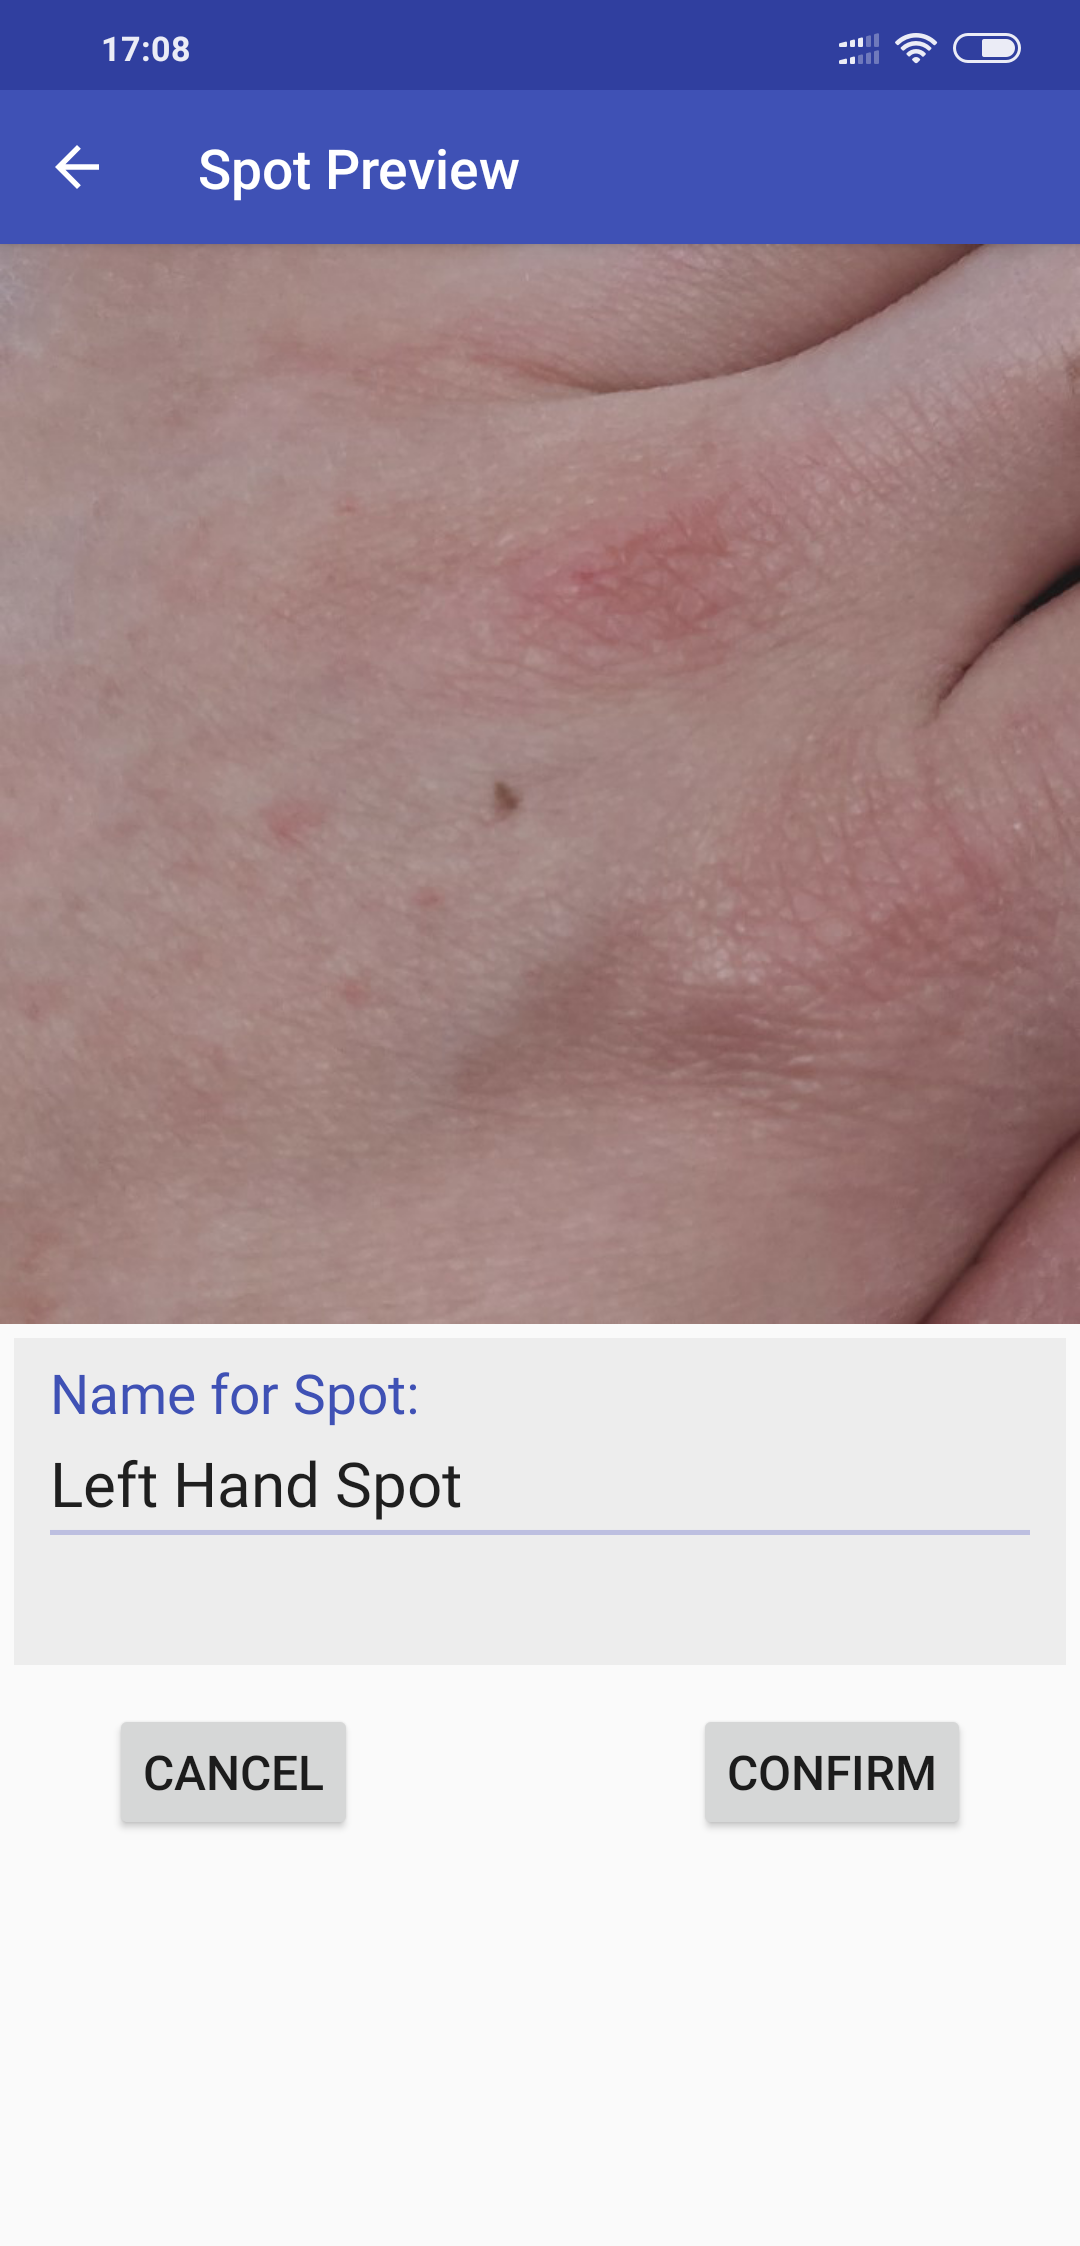
\includegraphics[height=10cm]{figures/confirmadd1.png}
        \caption{Redesigned AddSpot Activity Screen hiding the keyboard}
        \label{subfig:newaddspotkeyboard}
    \end{subfigure}%
     ~
    \begin{subfigure}[t]{0.5\textwidth}
        \centering
        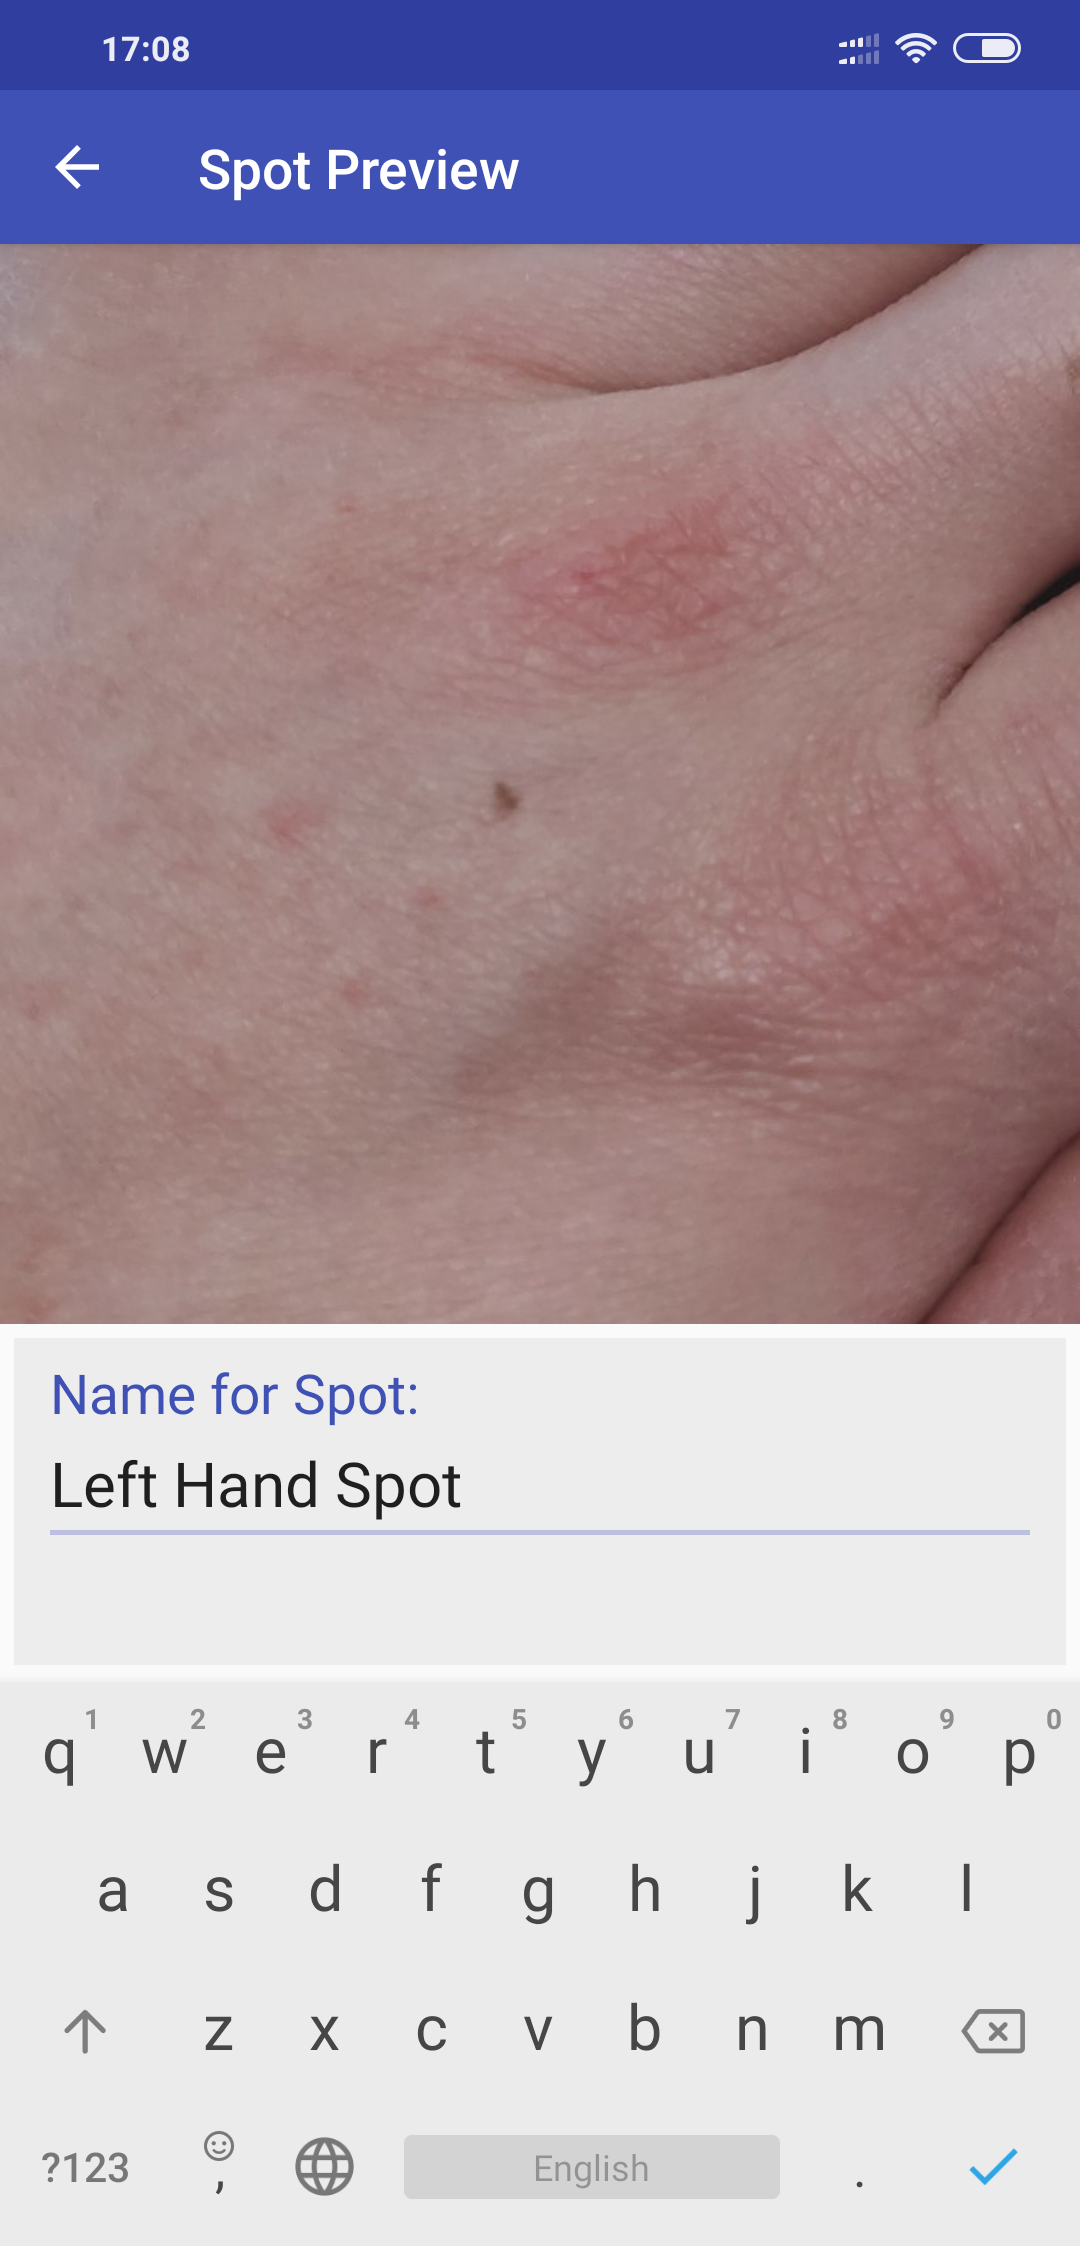
\includegraphics[height=10cm]{figures/addspot2.png}
        \caption{Redesigned AddSpot Activity after inputting text}
        \label{subfig:newaddspotnokeyboard}
    \end{subfigure}
    \caption{Progression of AddSpot Activity screens}
\end{figure*}

\subsection{Spot Image List Screen}

This screen displays a list of all taken photos of a spot (Figures \ref{subfig:spotimagelist} and \ref{subfig:spotimagelistcontext}), this enables the user to compare them over time, spotting any differences in appearance. Under the toolbar, a list of images is displayed. Each list item shows a thumbnail for each particular image, the name of the image, and the date on which the image was taken. The toolbar contains multiple action buttons, a back button to return to the previous screen, a "Compare" button to open the comparison contextual toolbar, and a "+" button to add a new photo to the list. Clicking on an item in the list would open a full-screen view of the image for better inspection.

When the user presses the first "Compare" button, the contextual action bar opens. This enters the user into selection mode, where tapping on any of the images highlight the image, indicating it has been selected. If two images are selected, the "Compare" button lightens up, taking the user to the side-by-side comparison screen.

When it comes to displaying the list of images, alternative design decisions for selecting spots to compare will be discussed in section \ref{CompareScreenDesignSection}. However, we can justify the choice of what information is displayed on each item. The thumbnail of each image is critical for the user to know which images they are selecting to compare, the name of each image contains the "JPEG" together with the timestamp of the photo. Arguably, this format could be more user friendly by including the name of the spot. This would require extra image renaming methods in the app implementation, but would further help the user identify images.

\begin{figure*}[t!]
    \centering
    \begin{subfigure}[t]{0.5\textwidth}
        \centering
        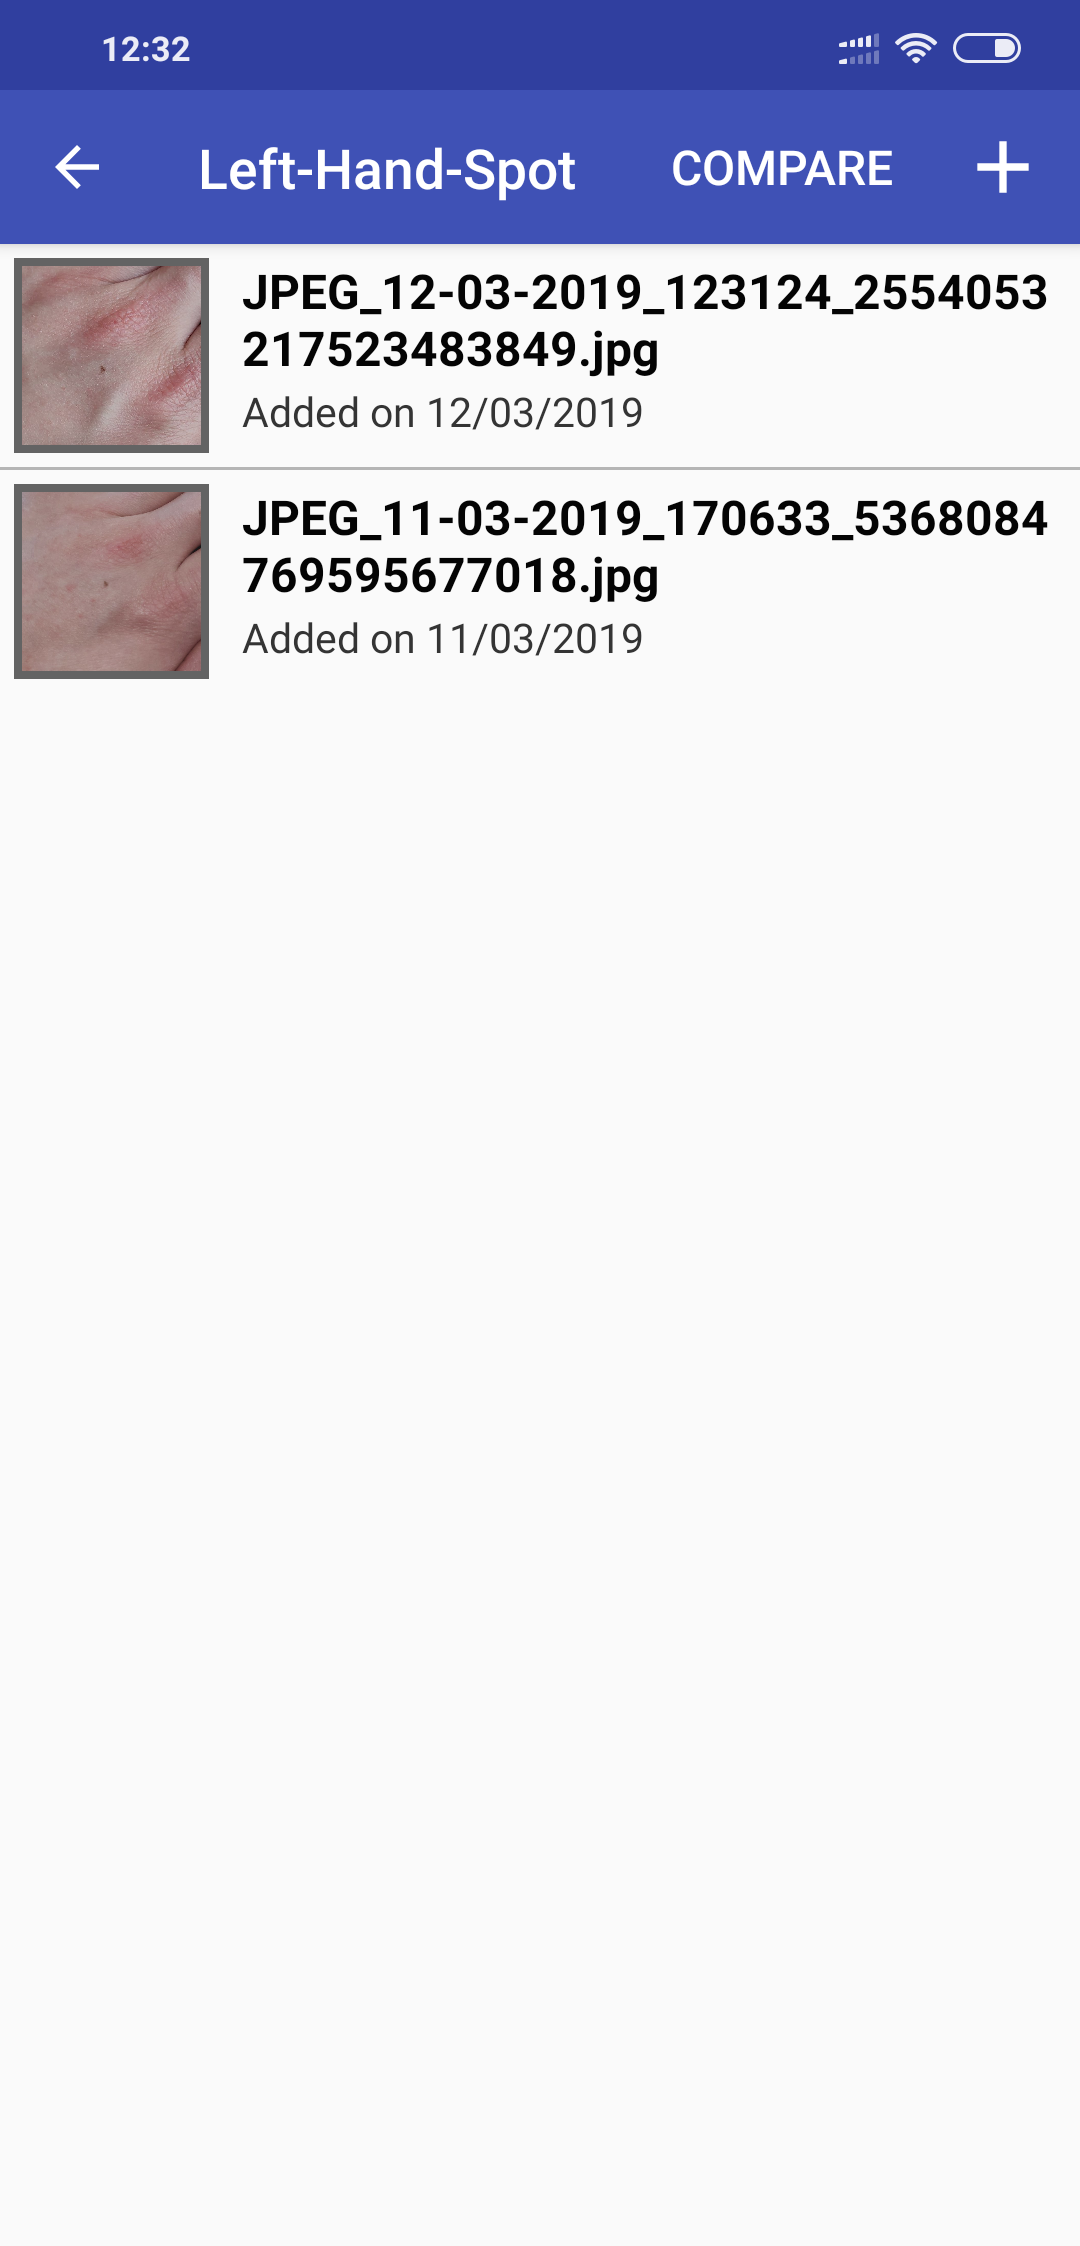
\includegraphics[height=10cm]{figures/spothistory2_android.png}
        \caption{List of images of a spot}
        \label{subfig:spotimagelist}
    \end{subfigure}%
    ~
    \begin{subfigure}[t]{0.5\textwidth}
        \centering
        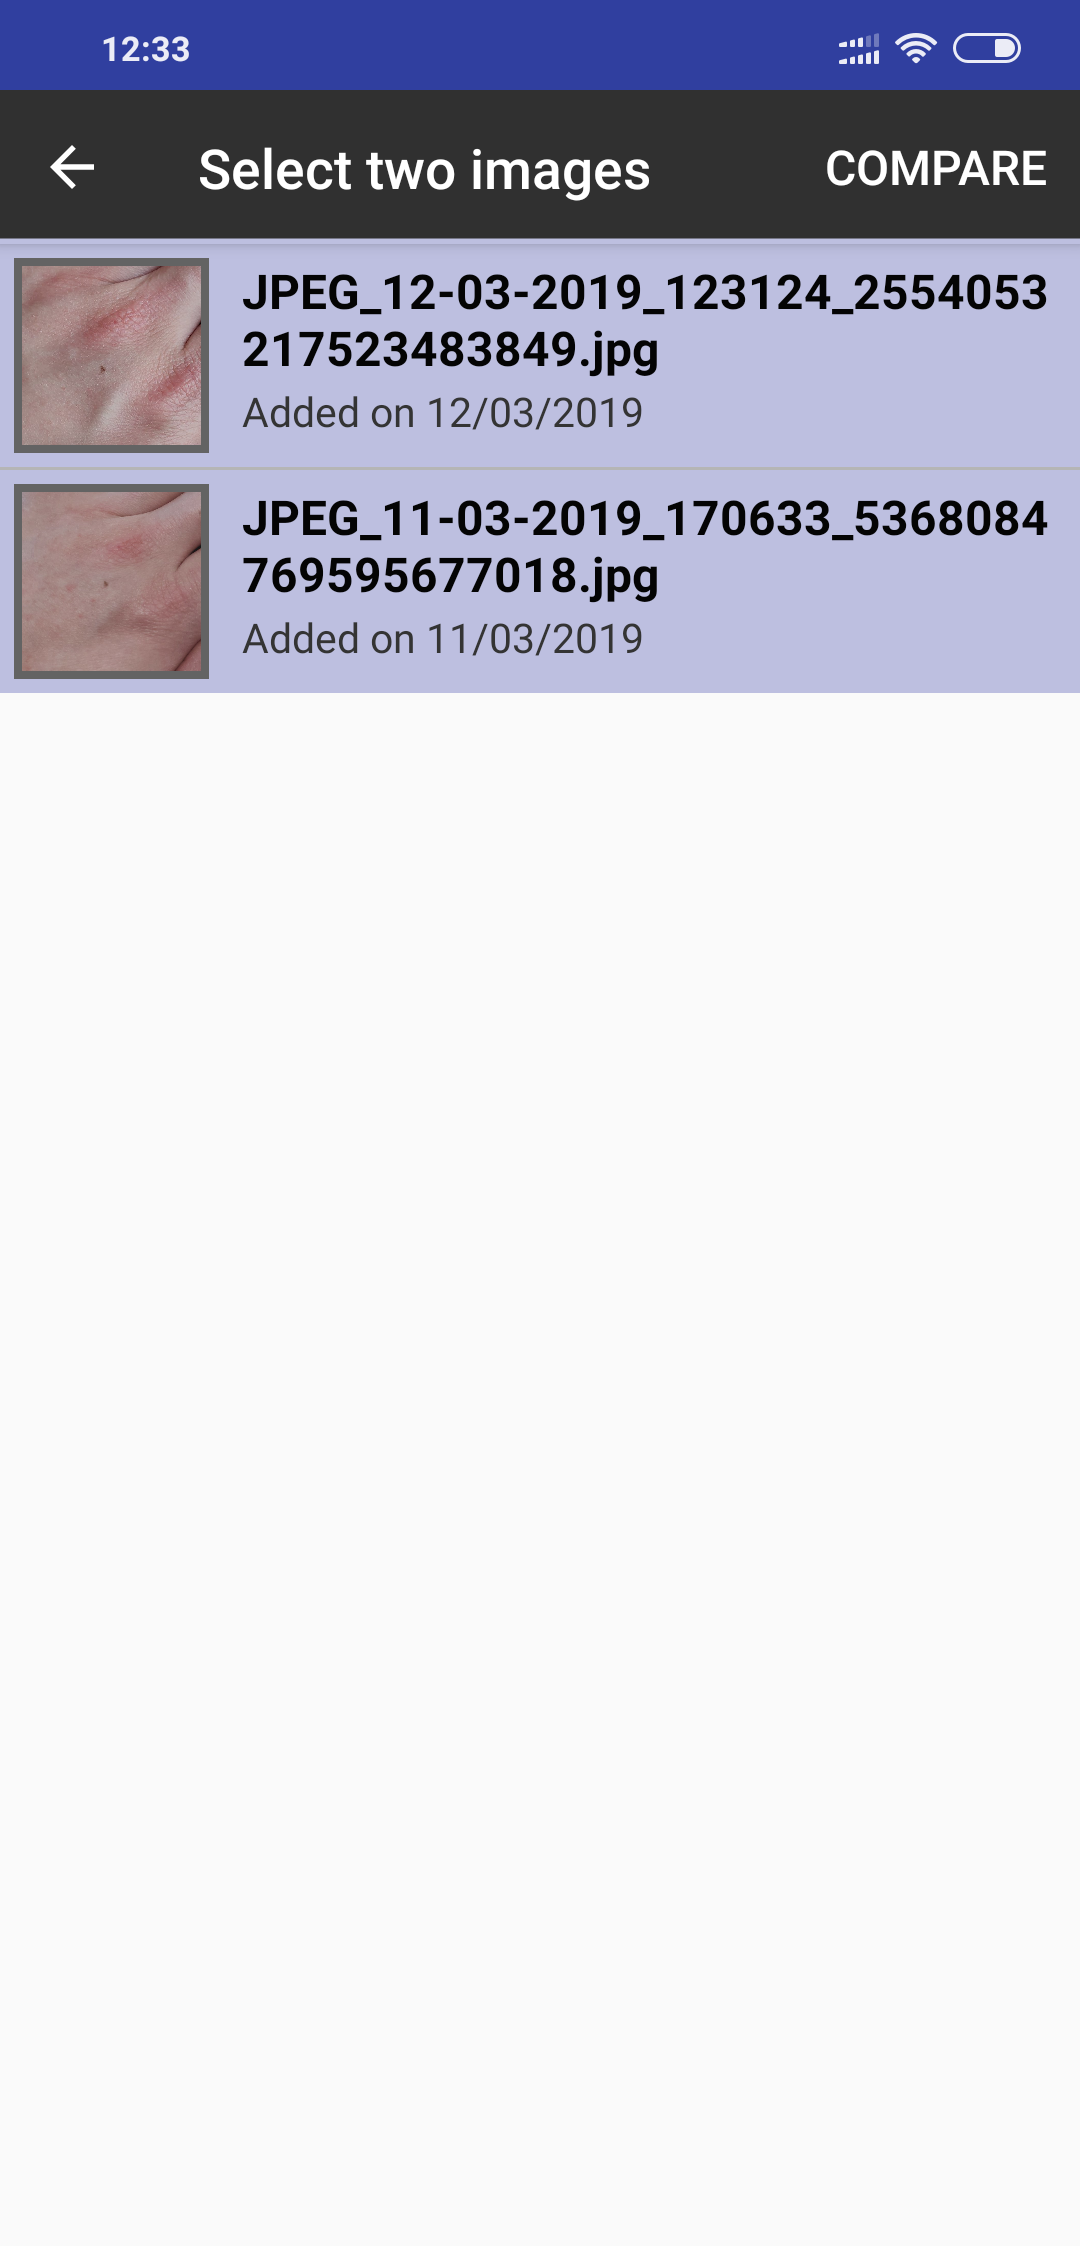
\includegraphics[height=10cm]{figures/compare1_android.png}
        \caption{Selecting images to compare}
        \label{subfig:spotimagelistcontext}
    \end{subfigure}
    \caption{SpotImageList Activity showing image selection for comparison}
\end{figure*}

\subsection{Comparing Spots Screen} \label{CompareScreenDesignSection}

The spot comparison screen (Figure \ref{fig:comparisonallfigures}) allows the user to closely inspect the differences between two previously selected images. It is the main feature that differentiates the app from a typical photo gallery app, also allowing the user to email both images to a doctor or user specified address.

A lot of thought was put into what the best way to compare images was. Two main approaches were considered. Figures \ref{fig:oldcompare1} and \ref{fig:oldcompare2} show the initial design, where all images are displayed in a "CarouselView", imitating a slideshow where the user can swipe left and right to compare all images. The main advantages and disadvantages of this design are highlighted below:
\begin{itemize}
    \item \emph{Smooth and Convenient} - Comparing images through swiping feels intuitive and natural to users.
    \item \emph{Memory Loss} - Continually loading all images of a spot can quickly exhaust the app's memory budget \cite{handlingbitmaps}. With certain older devices, issues still arise even after using efficient bitmap decoding libraries such as \emph{Glide}.
\end{itemize}

On the other hand, Figures \ref{subfig:spotimagelistcontext} and \ref{fig:newcompare1secondfig} show the second (and final) design for comparing images. This approach requires images to be selected in the spot image list screen and displays them statically one above the other. Each image takes up 50\% of the screen. Thoughts about this approach:
\begin{itemize}
    \item \textbf{Image Count} - It is unlikely for users to save more than 5 images of a spot. The appeareance of spots usually takes several months or years to change. This means that the user will not necessarily need to compare \textbf{all} the images of a spot, but the very first and last images would suffice.
    \item \textbf{Closer Zoom} - Loading only two images avoids any memory leaks, and removing the swipe interaction means images can take up the whole screen, enabling the user to inspect and compare the spots more easily.
    \item \textbf{Clunky Feel} - Selecting spots through a selection menu can feel more cumbersome to some users.
\end{itemize}

\clearpage
\begin{figure*}[t!]
    \centering
    \begin{subfigure}[t]{0.5\textwidth}
        \centering
        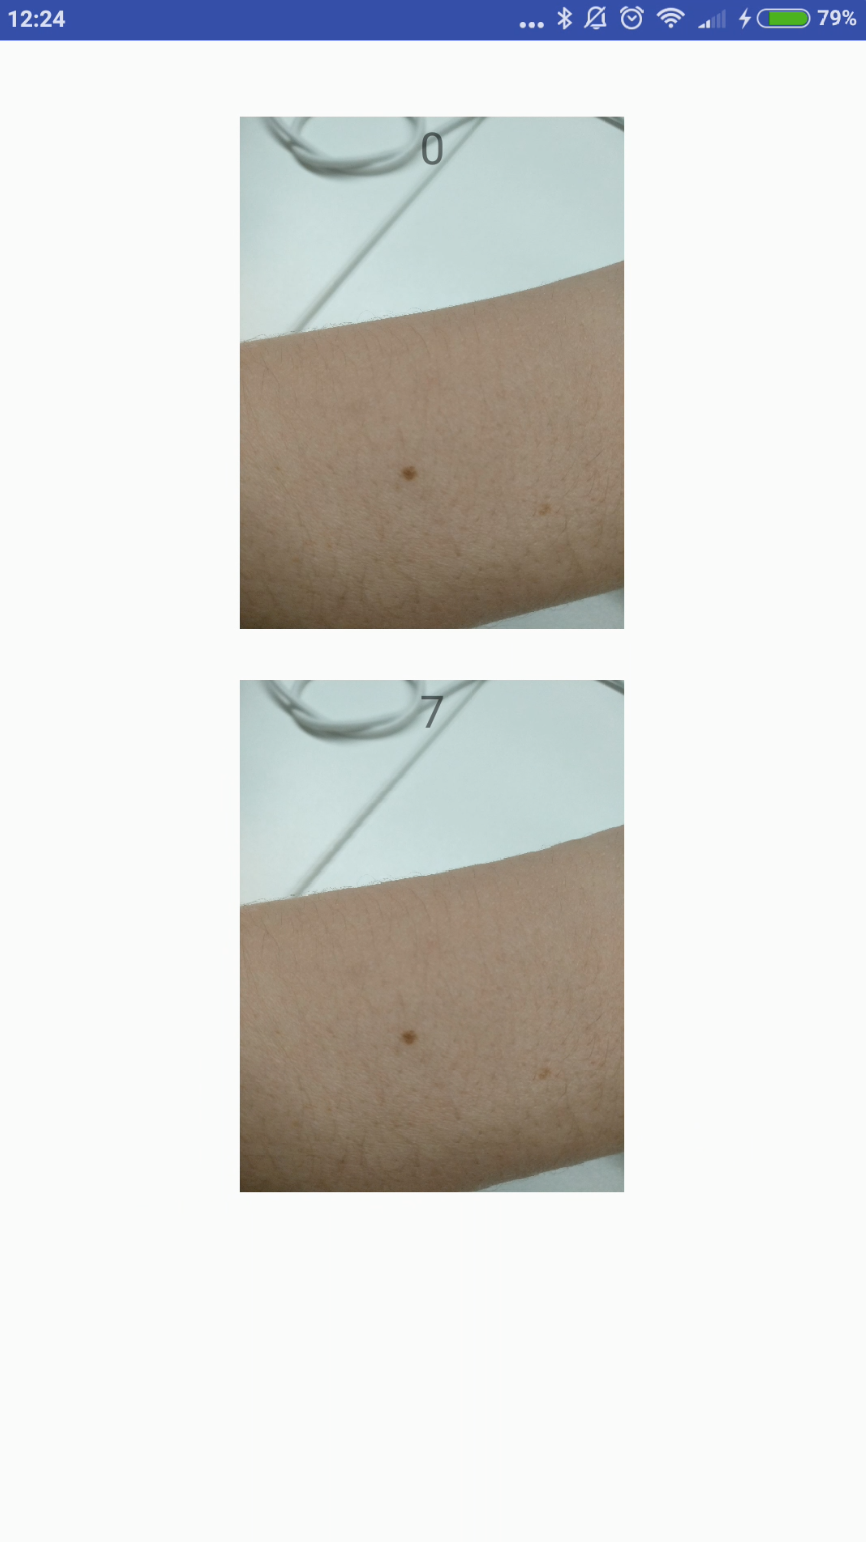
\includegraphics[height=10cm]{figures/oldcompare1.png}
        \caption{Display of initial compare screen design}
        \label{fig:oldcompare1}
    \end{subfigure}%
    ~
    \begin{subfigure}[t]{0.5\textwidth}
        \centering
        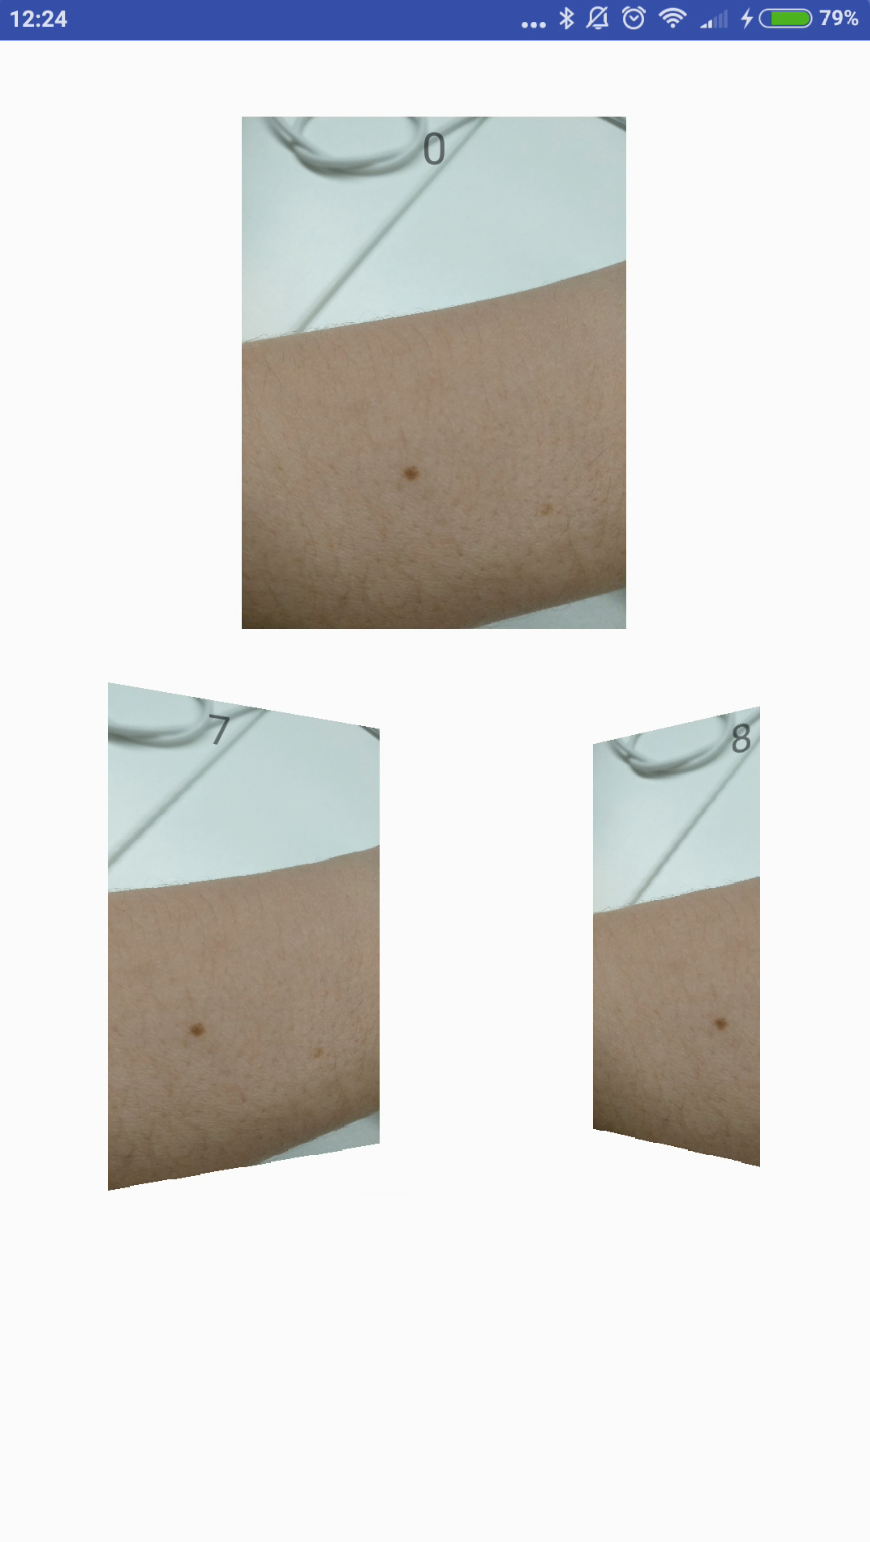
\includegraphics[height=10cm]{figures/oldcompare2.png}
        \caption{Comparing images can be done through swiping left and right}
        \label{fig:oldcompare2}
    \end{subfigure}
    \begin{subfigure}[t]{0.5\textwidth}
        \centering
        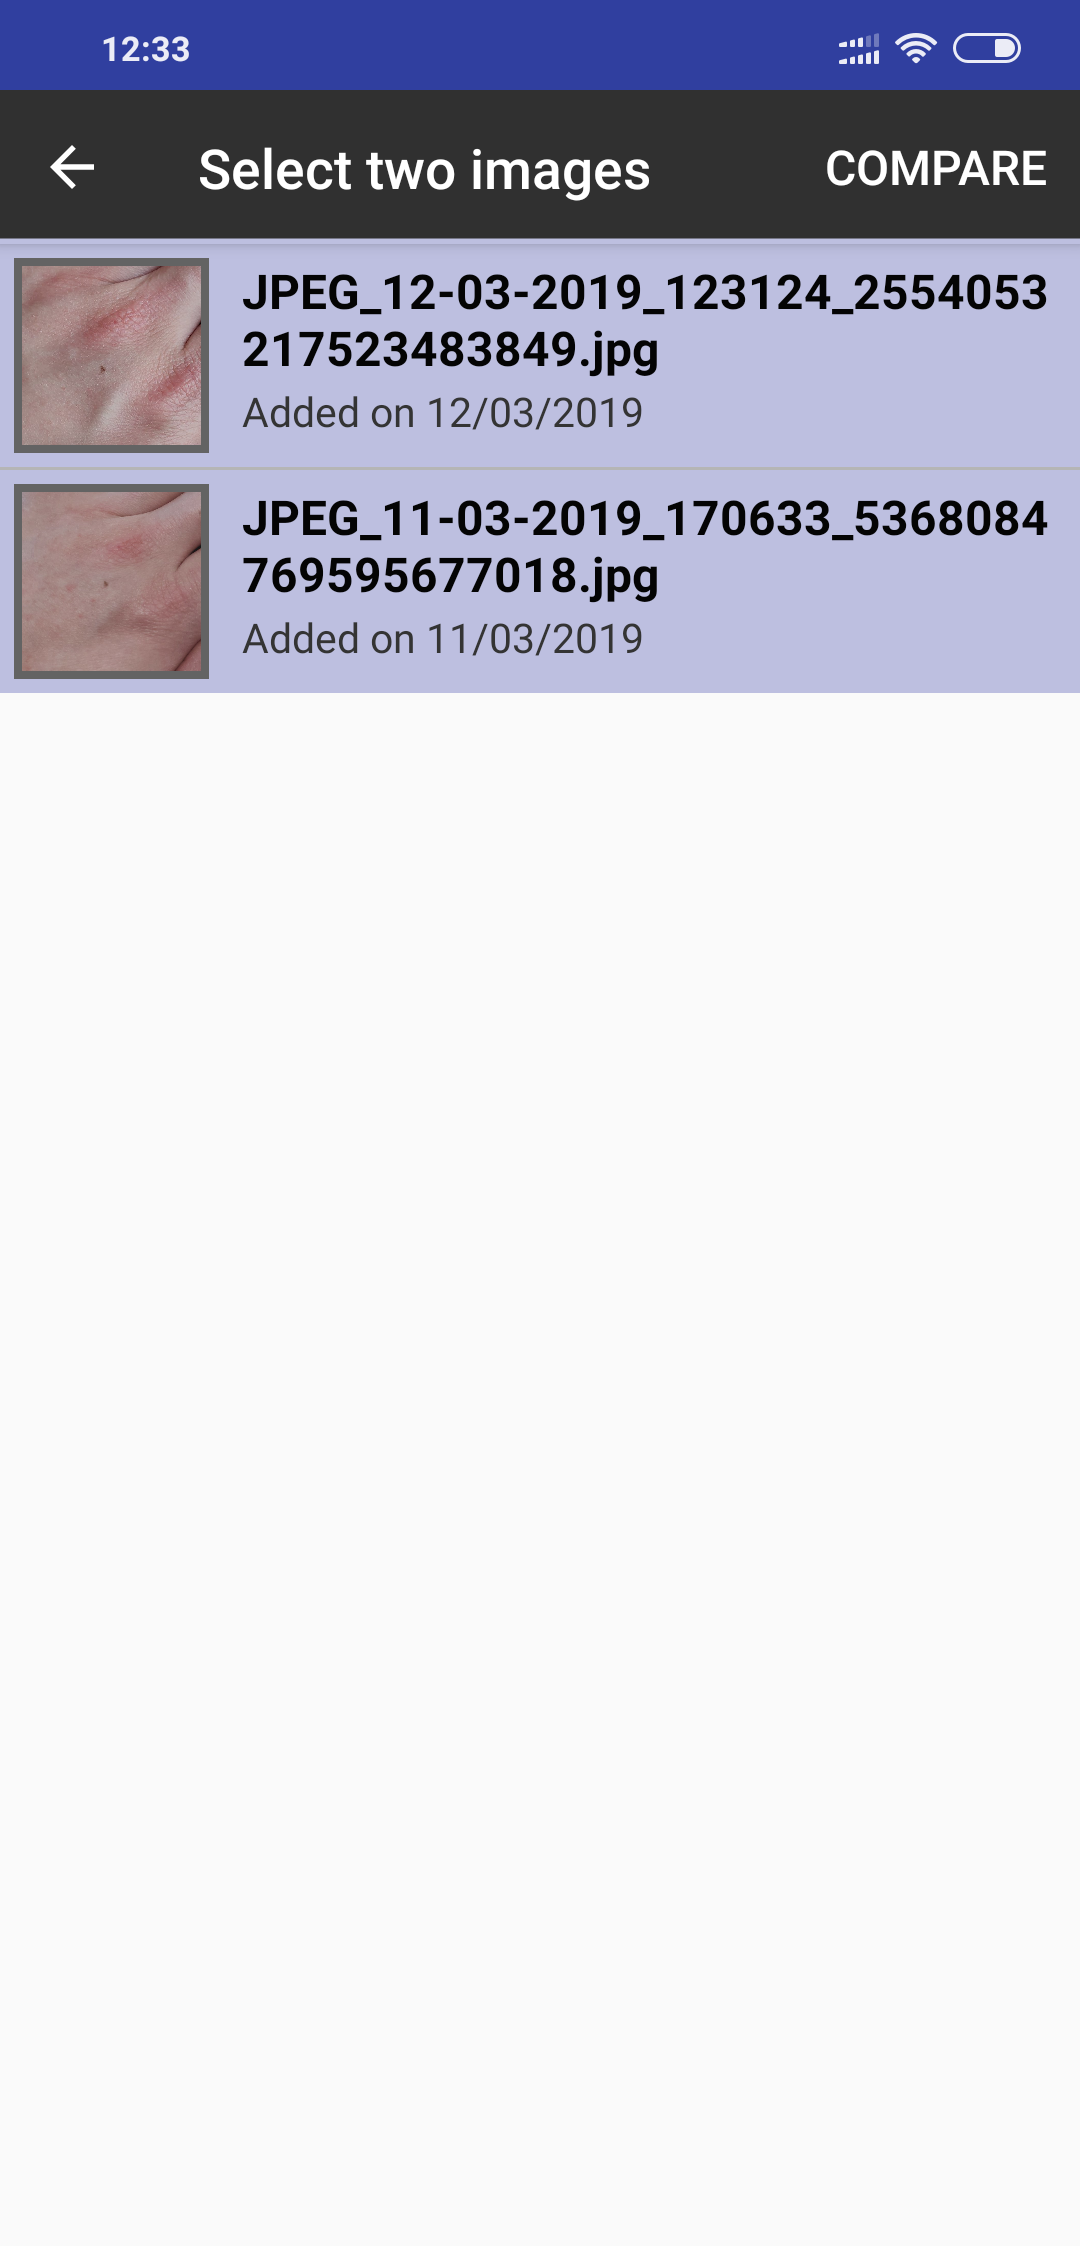
\includegraphics[height=10cm]{figures/compare1_android.png}
        \caption{Final compare screen image selection}
        \label{fig:newcompare1secondfig}
    \end{subfigure}%
    ~
    \begin{subfigure}[t]{0.5\textwidth}
        \centering
        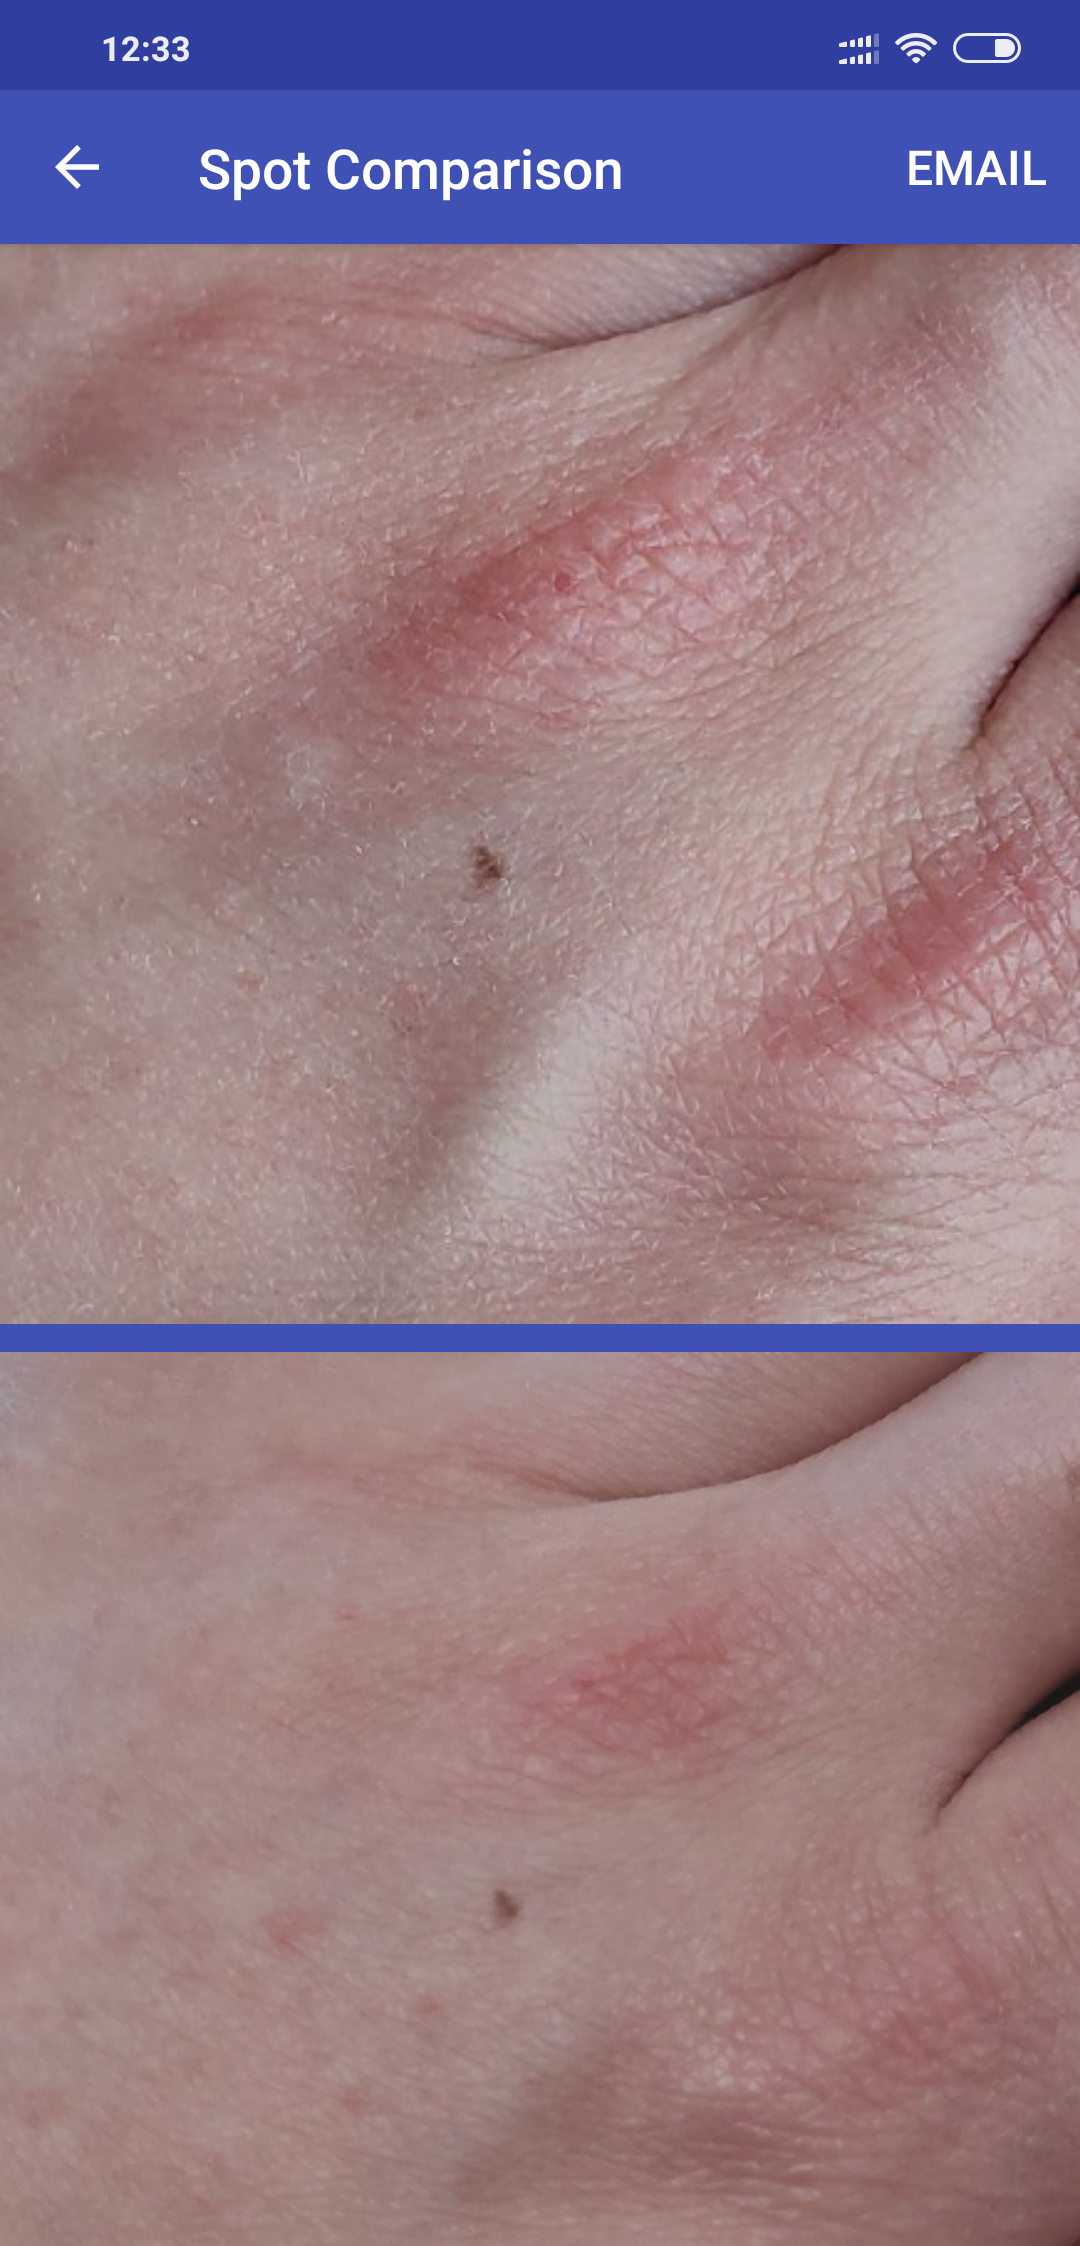
\includegraphics[height=10cm]{figures/compare2_android.png}
        \caption{Final design for comparing spot images}
        \label{fig:newcompare2}
    \end{subfigure}
    \caption{Progression of the Spot Comparison Screen}
    \label{fig:comparisonallfigures}
\end{figure*}

\subsection{Email Screen}
This screen is used to email the compared images to a doctor or another specified email address. There is no control over the design of this screen, as the "Email" button on the comparison screen simply opens a new email on the default email app on the user's device. The app automatically attaches both selected images and inserts a template text body (Figure \ref{fig:emailscreen}). 

\begin{figure}
    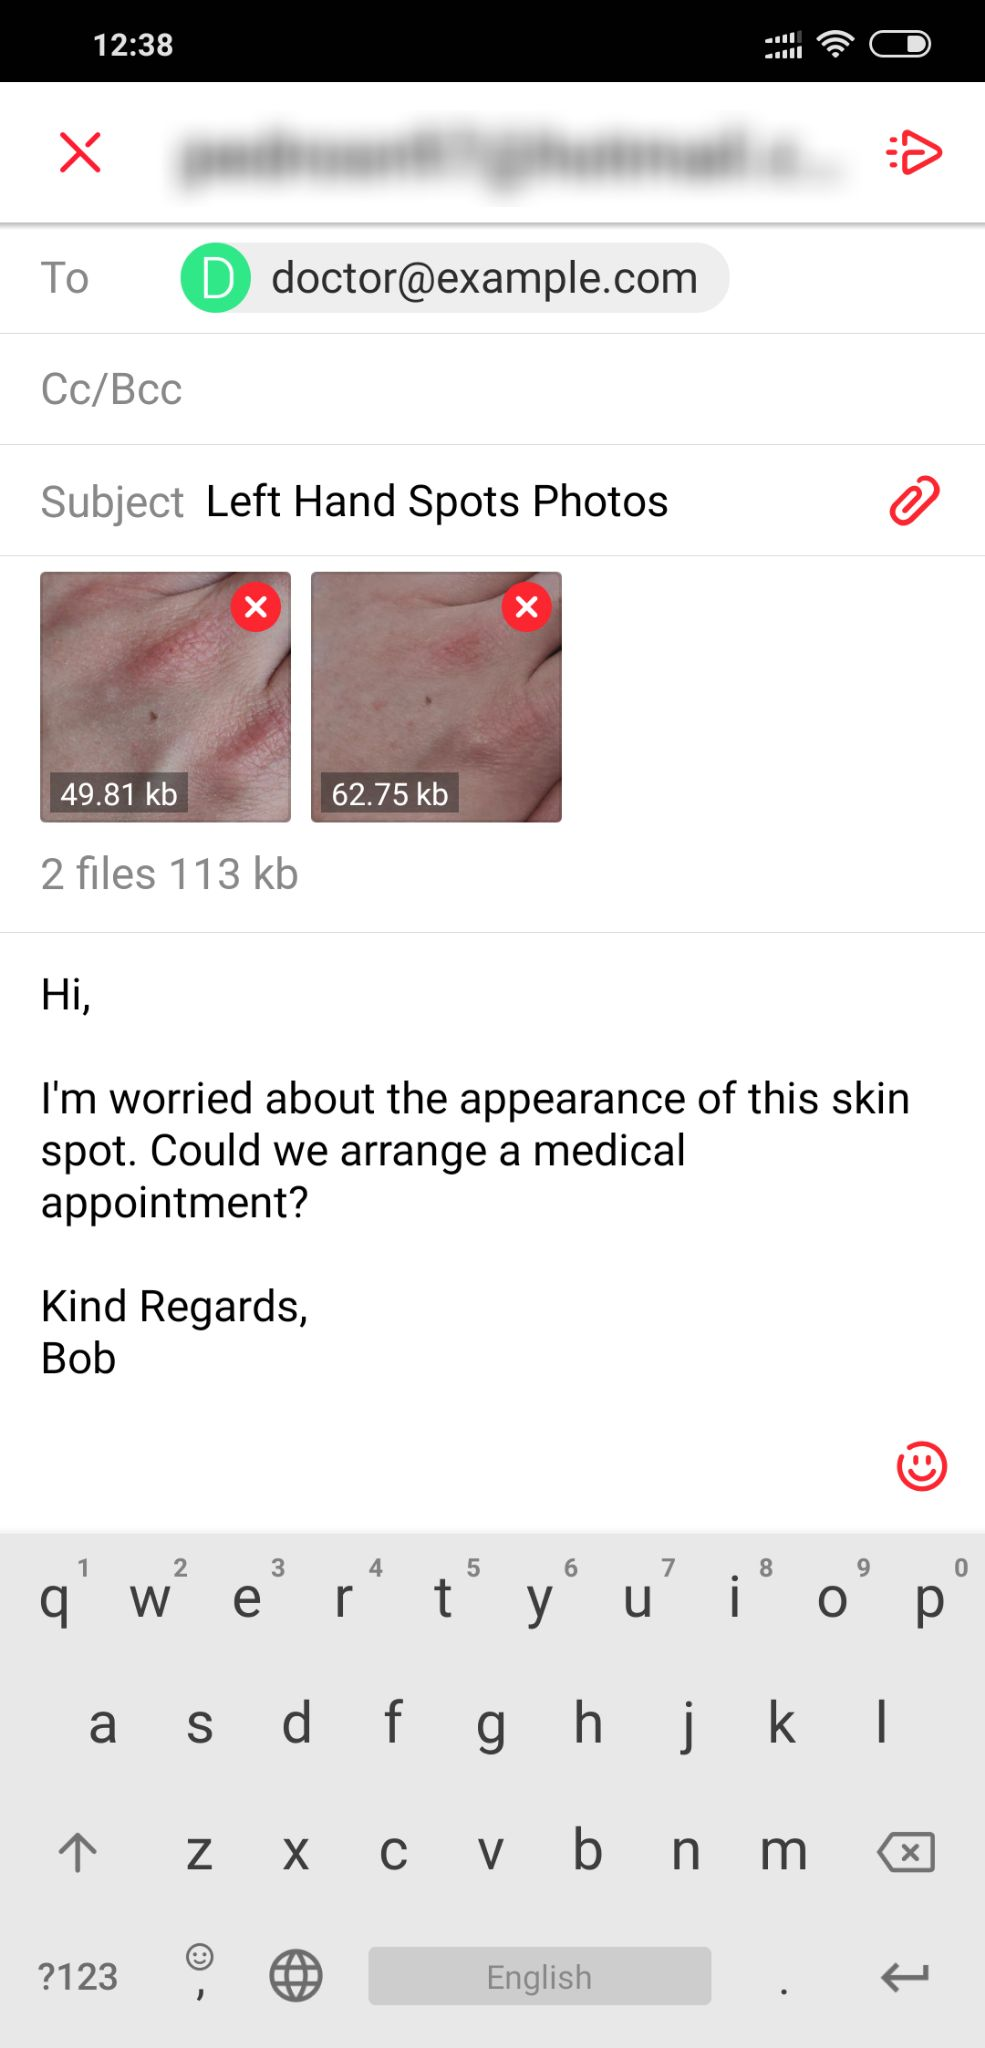
\includegraphics[height=10cm, center]{figures/email_android.jpg}
    \caption{Email Screen through the \emph{myMail} Android App}
    \label{fig:emailscreen}
\end{figure}

\section{Interactions}
\subsection{Navigation}
The app's navigation overview can be observed in Figure \ref{fig:nav_graph}, to summarise the interaction between the previously described screens: the app's home screen is the front perspective of the body screen. However, if the app has never been used before, the Information Screens will be displayed, giving the user a simple introduction to the app with some background information. From the home screen, the user can click on a body part to open the Old Spot screen for that body part, this would display a list of spots. The user can either add a new spot (Starting the Camera-Crop Process) or view a spot by tapping it. Tapping takes the user to the spot image list for the selected spot, following a similar design to the old spot screen, but in this case showing all the images for a particular spot. The user can select two images to compare (as shown in the Compare Screen), or once again start the Camera-Cropping process to add a new image of the spot. In the Compare Screen, the user can also choose to email both images to a specified email address.

As a recall from the technical requirements of the project, the goal was to develop an app with the following features:
\begin{enumerate}
        \item The user can add and name new spots. Subsequently, the user can add new images to a spot.
        \item The user is able to compare two images of a spot on the same screen.
        \item The ability to email both pictures to a doctor from within the app.
        \item Educational information screens towards skin cancer signs and usage of the app.
    \end{enumerate}
From a design perspective, all the core features have been accounted for, relying the success of the project on how successful we are at implementation and evaluation of the app.

\subsection{Navigation Redesign}
\label{nav_refactor}

The app's home screen and overall navigation was altered midway through the project. Initially, the app would welcome the user through a typical home screen menu. Figure \ref{fig:draft1menu} shows the layout of this home screen. The first 3 buttons would all lead to the body screen, after which either the camera or list of spots would be displayed (depending on the main menu option selected). As would seem apparent, this design is very redundant, as all three options would essentially lead the user to the same screens. This lead to re-factoring the whole design of the app, shifting towards a body interface home-screen (Figure \ref{fig:nav_graph}). From this point, actions to add spots, add photos, or compare spots had to be implemented within the \emph{OldSpotScreen} and \emph{SpotImageScreen} Activities, since the user woudn't be selecting these from the main menu. Benefits and drawbacks of this approach include:
\begin{itemize}
    \item \textbf{Decrease redundancy} - The user doesn't have to go through the same 2 screens for every different action, saving time and delivering a more efficient interface 
    \item \textbf{Loss of clarity} - Having a main menu with options has its merits, as the user knows exactly what action they are currently doing, preventing them from getting lost within the app. This is particularly true with older users.
    \item \textbf{Flexibility} - The user can easily switch between actions without returning to the main menu, for example, if a user wanted to add a new spot A, then  add an updated photo of a different spot B, and finally compare two images of spot B, they could easily do this by entering the different body part spot lists, without requiring the user to return to the main menu screen three times.
\end{itemize}
Overall, the conclusion was that the main menu design in figure \ref{fig:firstappdraft} would only be suitable if users only completed 1-2 within every app use. With this unrealistic expectation, it was decided to shift to the body home screen design.
\clearpage
\begin{figure*}[t!]
    \centering
    \begin{subfigure}[t]{0.5\textwidth}
        \centering
        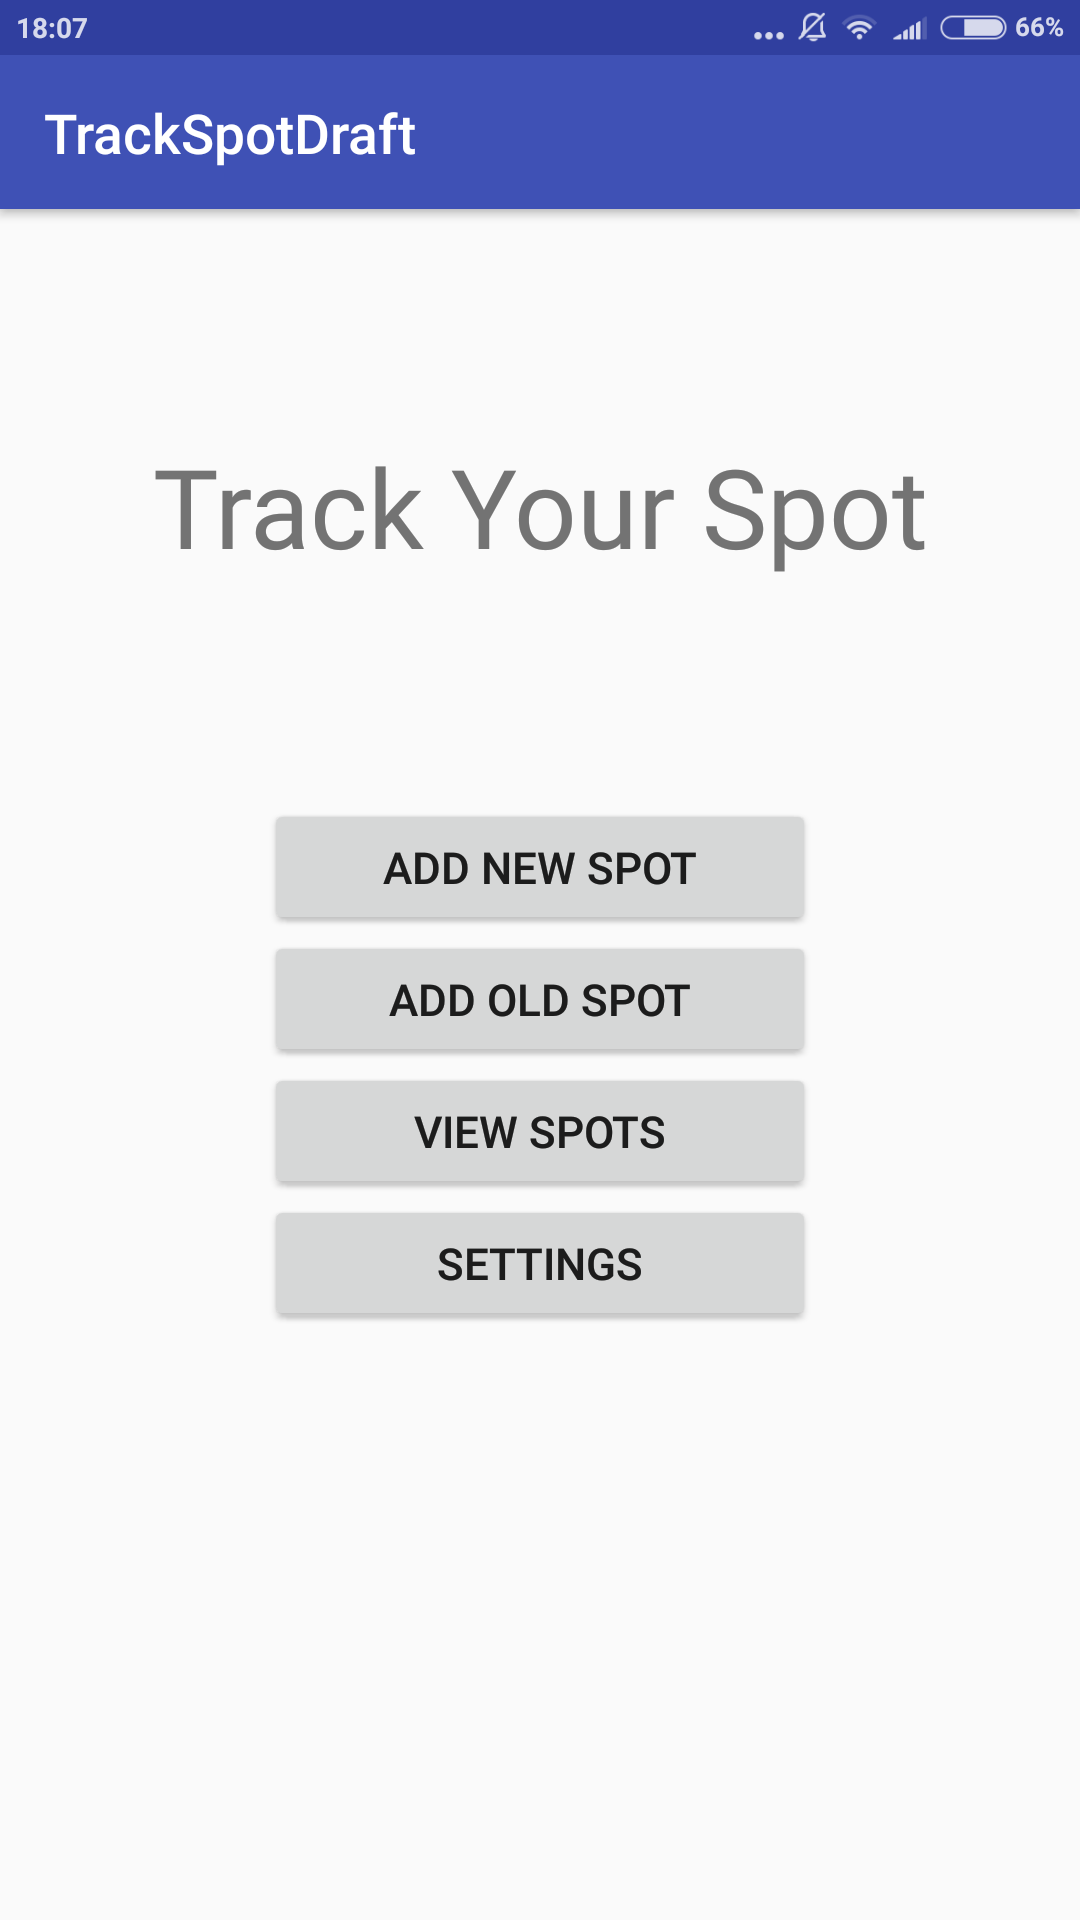
\includegraphics[height=10cm]{figures/draft1menuscreen.png}
        \caption{First app draft home screen}
        \label{fig:draft1menu}
    \end{subfigure}%
    ~
    \begin{subfigure}[t]{0.5\textwidth}
        \centering
        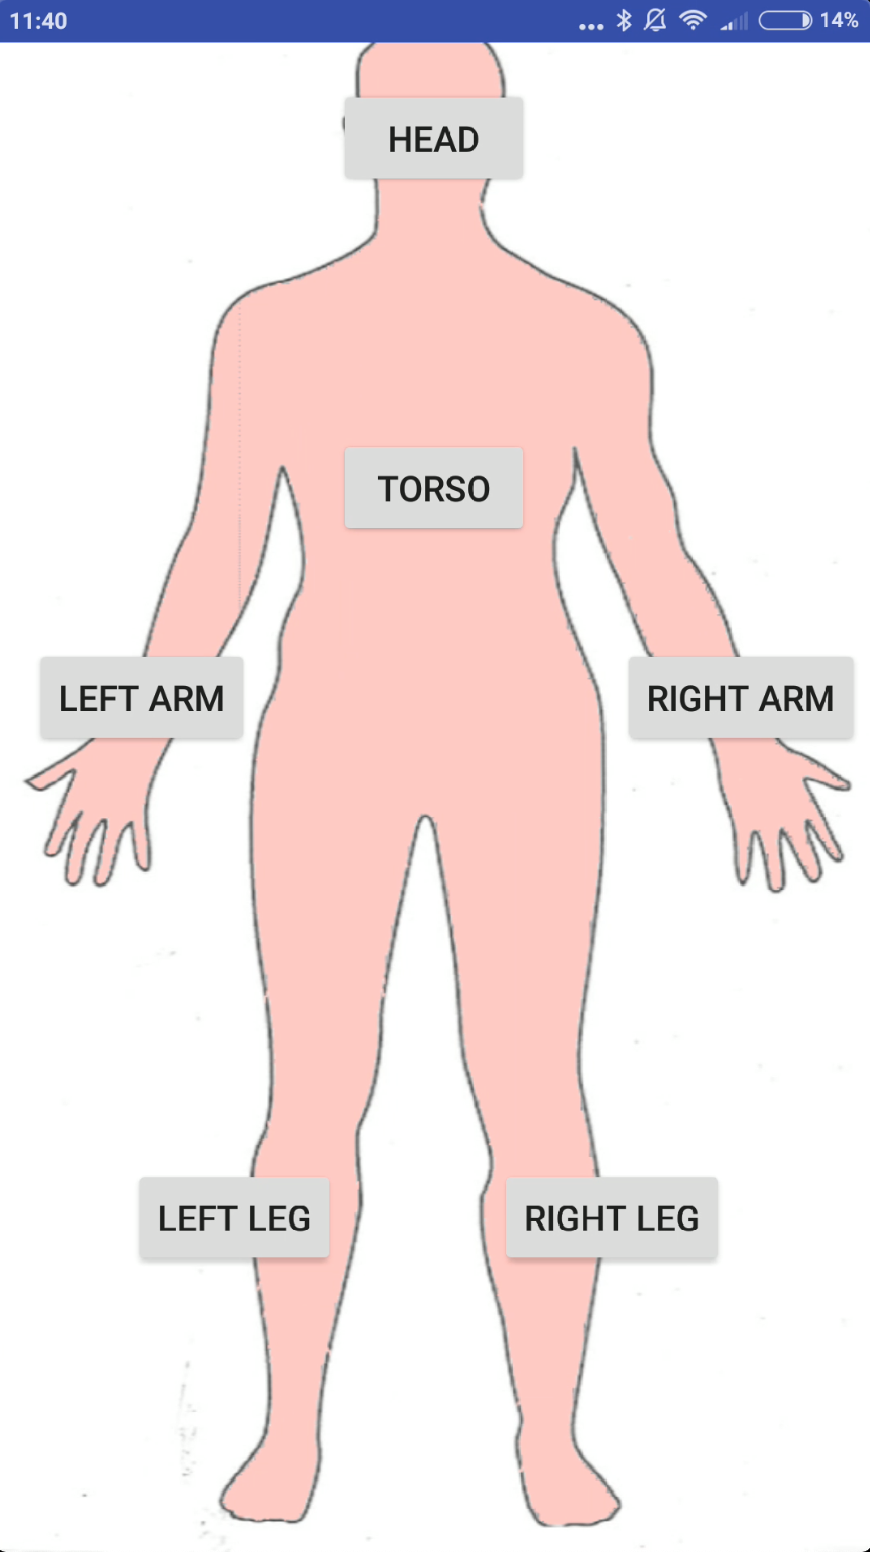
\includegraphics[height=10cm]{figures/draft1bodyscreen.png}
        \caption{First app draft body screen}
    \end{subfigure}
    \caption{Navigation menu of first app draft}
    \label{fig:firstappdraft}
\end{figure*}
\clearpage
\begin{figure}
    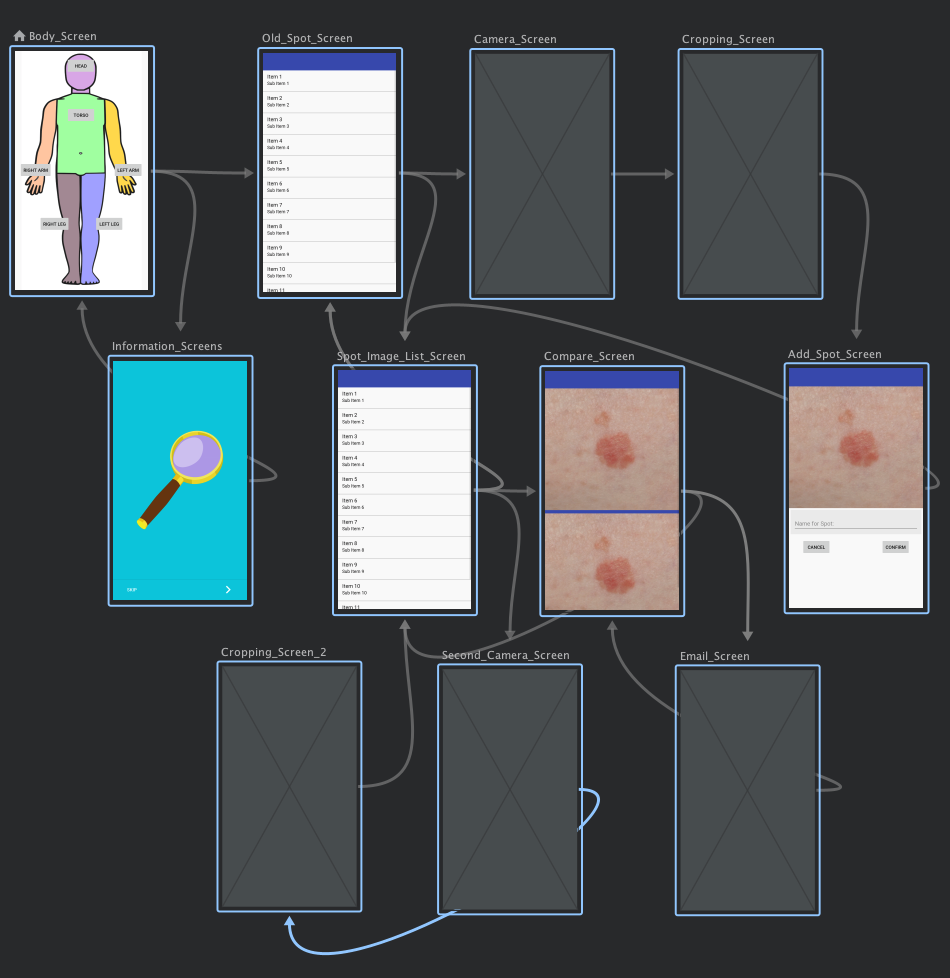
\includegraphics[width=1.2\textwidth, center]{figures/nav_graph.png}
    \caption{Navigation Graph}
    \label{fig:nav_graph}
\end{figure}
\chapter{Architecture and Implementation}
\section{Main Components}
This section encompasses the architecture behind the app. Each screen will include information about methods and algorithms used, accompanied by Activity UML diagrams to better visualise what the code does for the user and how it interacts with the app's UI. Note that Android's default "back" button allows the user to always return to a previous screen in the app. To avoid cluttering, obvious "back" operations have been omitted from UML diagrams. In addition, note that code listings only contain subsets of the code, a lot of the less "interesting" code has been omitted from the report.

The language of choice is \emph{Kotlin}, the leading programming language in Android app development \cite{sagar_2019}.  Kotlin is a fully Android-focused language running on the \emph{Java Virtual Machine}. It is extensively supported by \emph{Android Studio}, the official Android IDE. Both Kotlin and Android Studio have been developed by \emph{JetBrains}. For these reasons, the option of developing the app in Java was quickly dismissed. Any relevant libraries used within activities can be found in the bibliography. It might be useful to re-read Section \ref{definitionssection} for a better understanding of the technical terms used throughout this section.

\subsection{App Opening and Information Screens}

In Android development, we use \emph{Shared Preferences} as a way of saving the user's app data to be used in the future. In our implementation, we don't necessarily need a heavy use of shared preferences, as images are directly saved and scanned from storage (see Section \ref{sec:filestructure}). However, we can utilise them to save small user settings or specific variables. In the app's homescreen, we use this tool to check if the user has already completed the tutorial in the past. Observe code listing \ref{lst:infoscreens}, the code first checks if the user has just returned from another screen, selecting the right tab "front" or "back" from where the user started their action, this code is irrelevant if the app has just been opened. On lines 11-15, we make use of a boolean "TutorialDone" to track if the user has already completed the tutorial information screens, this is accomplished through the \code{getPreferences}, \code{getBoolean} and \code{putBoolean} methods.

As displayed in Figure \ref{fig:InfoDiagram}, the user can return to the body screen by completing or skipping the tutorial. Contrarily, pressing the "i" button allows the user to retake the tutorial. 

\begin{lstlisting}[caption={Displaying Information Screens}, label={lst:infoscreens}, language=Kotlin]
//Check if the user has pressed the back button
selectedBodySide = if (intent.hasExtra("selectedBodySide")) {
    intent.getStringExtra("selectedBodySide")
} else {
    "front"
}
createTabs(selectedBodySide) //Displays front and back tabs
//Android way of retrieving previous app data
val sharedPref = this.getPreferences(Context.MODE_PRIVATE) ?: return
val isTutorialDone = sharedPref.getBoolean("TutorialDone", false)
if (!isTutorialDone) {
    //If app first time use, show tutorial
    sharedPref.edit().putBoolean("TutorialDone", true).apply()
    val intent = Intent(this, IntroActivity::class.java)
    startActivity(intent)
}
\end{lstlisting}

\begin{figure}
    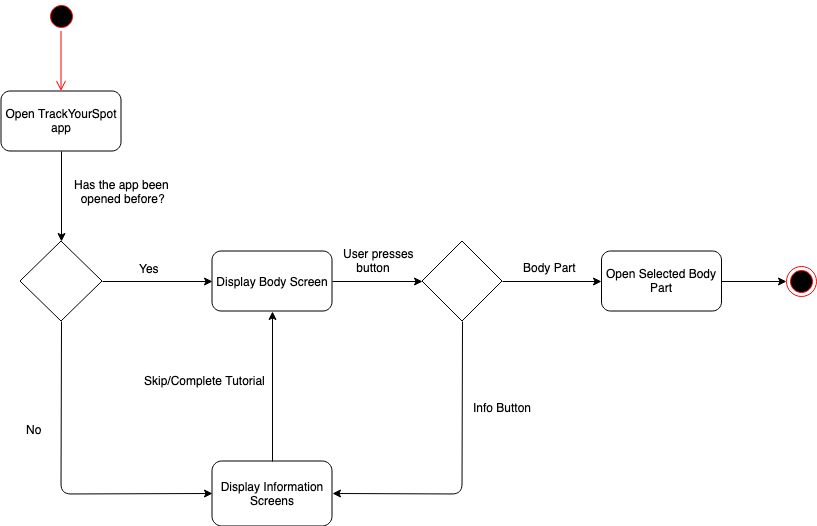
\includegraphics[width=1.2\textwidth, center]{figures/InfoDiagram.png}
    \caption{UML Activity Diagram for Info Screens}
    \label{fig:InfoDiagram}
\end{figure}

\subsection{CameraOpeningActivity} \label{sec:cameraarch}

\begin{figure}
    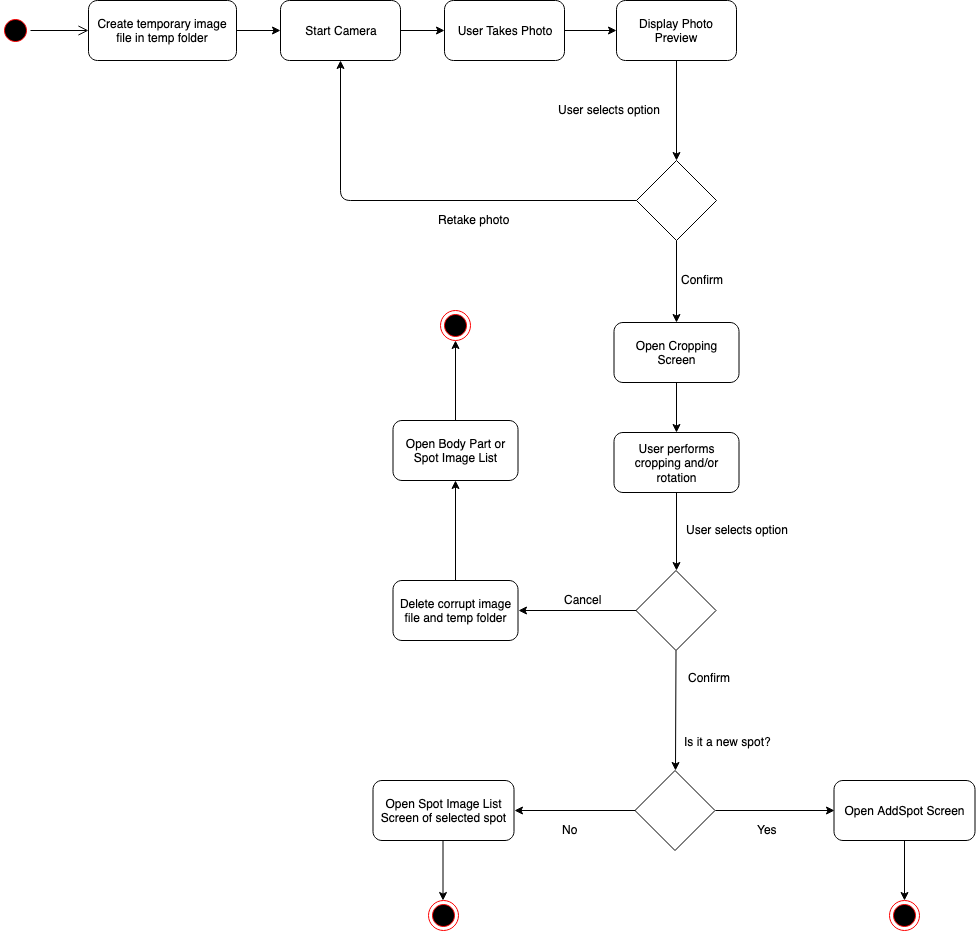
\includegraphics[width=1.2\textwidth, center]{figures/CameraScreen.png}
    \caption{UML Activity Diagram for the Camera Activity}
    \label{fig:CameraScreen}
\end{figure}
To explain the implementation of the \emph{OldSpotList} and \emph{SpotImageList} activities, we first have to break down the \emph{CameraOpeningActivity} class. This class was created so that the two mentioned activities could share the \code{createImageFile} and \code{dispatchTakePictureIntent} methods, avoiding any redundant code. \code{createImageFile()} is used for creating a temporary empty image file in storage for the image to be taken, and \code{dispatchTakePictureIntent()} starts the actual camera app to save a new picture into this image file. The code has been adapted from the Android docs \cite{androiddevelopers3}, as these methods are widely used across any Photo taking app, comments have been added for clarification.

Take the \emph{OldSpotList} activity as an example. The user first selects a body part. They are then presented with the list of spots from that selected body part. Once the user presses the "+" button, the \code{ dispatchTakePictureIntent()} method would be called (Code Listing ~\ref{lst:dispatchTakePictureIntent}). The spotDirectory argument contains the path of where the photo will be saved, this could be something similar to:
\begin{verbatim}
/storage/emulated/0/Pictures/TrackYourSpot/front/torso/worryingspot/
\end{verbatim}
In line 8, the \code{createImageFile()} method first tries to create a temporary image file at the given path. It uses the current date and time to create a unique timestamp string (Code Listing ~\ref{lst:createImageFile}). This ensures no two images will have the same name. Next, the method checks if the spotDirectory path exists in storage, creating them through the \code{mkdirs()} method if needed. Once we have the directory, it creates the temporary file by concatenating the "JPEG\textunderscore" prefix, the timestamp, and the ".jpg" file extension. Back to the \code{dispatchTakePictureIntent} method, we need to find the \emph{URI} of the photoFile. The URI variable is passed on to the Intent in charge of starting up the Camera. For compatibility reasons, we have to check the device's Android version, as SDKs older than Lollipop require a different way of attaching intent data to the camera intent.

To see how this code interacts with the app's UI and navigation screens, take a look at Figure \ref{fig:CameraScreen}. The diagram also shows the paths the app takes if the user cancels the camera or cropping processes midway through. Since the camera process is based around temporary image files, these have to be dealt with accordingly.

\clearpage

\begin{lstlisting}[caption={Starting the Camera}, label={lst:dispatchTakePictureIntent}, language=Kotlin]
fun dispatchTakePictureIntent(spotDirectory: String) {
        Intent(MediaStore.ACTION_IMAGE_CAPTURE).also {
            takePictureIntent ->
            // Ensure that there's a camera activity to handle the intent
            takePictureIntent.resolveActivity(packageManager)?.also {
                // Create the File where the photo should go
                val photoFile: File? = try {
                    createImageFile(spotDirectory)
                } catch (ex: IOException) {
                    ... //Display error message
                }
                // Continue only if the File was successfully created
                photoFile?.also {
                    //Get the image file's URI
                    val photoURI: Uri = FileProvider.getUriForFile(
                            this, "my.package.name.provider", it)
                    //For compatibility issues, we need to check the device's
                    //Android version and add write permissions accordingly.
                    if (Build.VERSION.SDK_INT >= Build.VERSION_CODES.LOLLIPOP) {
                        takePictureIntent.addFlags(Intent.FLAG_GRANT_WRITE_URI_PERMISSION)
                    } else {
                        val clip = ClipData.newUri(contentResolver, "clipData", photoURI)
                        takePictureIntent.clipData = clip
                        takePictureIntent.addFlags(Intent.FLAG_GRANT_WRITE_URI_PERMISSION)
                    }
                    //Open Camera App
                    takePictureIntent.addFlags(Intent.FLAG_GRANT_READ_URI_PERMISSION)
                    takePictureIntent.putExtra(MediaStore.EXTRA_OUTPUT, photoURI)
                    startActivityForResult(takePictureIntent, OldSpotScreen.REQUEST_TAKE_PHOTO)
                }
            }
        }
    }
\end{lstlisting}



\begin{lstlisting}[caption={Creating an Image File}, label={lst:createImageFile}, language=Kotlin]
private fun createImageFile(spotDirectory: String): File {
        //Used for creating a unique name for the image file
        val timeStamp: String = SimpleDateFormat("dd-MM-yyyy_HHmmss").format(Date()) 
        //If needed, create the folder for the spot.
        val newDir = File(spotDirectory)
        if(!newDir.exists()) newDir.mkdirs()
        //Create a temporary image file
        return File.createTempFile(
                "JPEG_${timeStamp}_",
                ".jpg",
                newDir
        ).apply {
            //Saves the image path in String format for later use.
            currentFullPhotoPath = absolutePath
        }
\end{lstlisting}

\clearpage

%If you uncomment you have to explain it
%\begin{lstlisting}[caption={Camera and Cropping Output}, label={lst:cameraoutput}, language=Kotlin]
%//If Cropping has been done successfully
%if (resultCode == RESULT_OK && requestCode == UCrop.REQUEST_CROP) {
%    //Open Spot Image list screen for that specific spot
%    val intent = Intent(this, SpotImageList::class.java)
%    //Pass on spot name and directory to the image list
%   intent.putExtra("spotName", spotName)
%    intent.putExtra("spotDirectory", spotDirectory)
%    intent.putExtra("selectedBodyPart", selectedBodyPart)
%    intent.putExtra("selectedBodySide", selectedBodySide)
%    startActivity(intent)
%}
%
%//If Photo has been taken successfully
%f (requestCode == REQUEST_IMAGE_CAPTURE && resultCode == Activity.RESULT_OK) {
%    //Check if the photopath is valid (eg. is a jpg file in storage)
%    if (isValidPhotoPath(currentFullPhotoPath)) {
%        //Start uCrop cropping screen with specific UI properties
%        val cropOptions = UCrop.Options().apply {
%            setAllowedGestures(UCropActivity.NONE, UCropActivity.NONE, UCropActivity.NONE)
%            setShowCropGrid(false)
%            setToolbarColor(ContextCompat.getColor(applicationContext, R.color.blue))
%           setActiveWidgetColor(ContextCompat.getColor(applicationContext, R.color.blue))
%            setStatusBarColor(ContextCompat.getColor(applicationContext, R.color.blue))
%            setShowCropFrame(true)
%        }
%        //Choose the same source and destination for the cropped image (Overwrite it)
%       UCrop.of(Uri.parse("file://$currentFullPhotoPath"),
%                Uri.parse("file://$currentFullPhotoPath"))
%                .withAspectRatio(1.toFloat(),1.toFloat())
%                .withOptions(cropOptions)
%                .start(this)
%        }
%    }
%
%//If photo hasn't been taken (eg. user presses the back button)
%if (resultCode != RESULT_OK && isValidPhotoPath(currentFullPhotoPath)) {
%    //Delete the corrupt image file
%    File(currentFullPhotoPath).delete()
%    val intent = intent
%    finish()
%    startActivity(intent)
%}
%\end{lstlisting}

\subsection{Old Spot List Screen}

The old spot list screen extends the abstract class \emph{CameraOpeningActivity}. The code in this activity accomplishes the following tasks (See UML Diagram in Figure \ref{fig:OldSpotList}):
\begin{enumerate}
    \item Load all saved spots from storage
    \item Display spots with thumbnails and other info in a list format
    \item Start camera automatically or after the user's button click, checking permissions accordingly
\end{enumerate}
To display the list of spots of a selected body part, we run the algorithm in code listing \ref{lst:retrieveSpots}. This algorithm scans through directories and reads every spot name and path repeatedly. It first initialises empty arrays for spotNames, spotDetails, spotPaths and thumbnails (Lines 1-4). Using the  \code{walk()}  method, it loops through every file inside the \code{../TrackYourSpot/bodypart/} directory. Setting the \code{maxDepth} parameter to 1 ensures only the top level folders inside these are read, in other words, only the spot names, but nothing inside these directories. Index 0 contains the root folder, therefore we choose to ignore it as it does not provide a spotName. Inside each of these spotName folders, we perform a 1-depth walk again, this time selecting only the file at index 1, which would contain the first image taken of a spot. We then use this image's path to display a thumbnail for each spot.

\clearpage
\begin{lstlisting}[caption={Loading Old Spots}, label={lst:retrieveSpots}, language=Kotlin]
var spotNames = emptyArray<String>() //Spot Names
var spotDirectories = emptyArray<String>() //Spot paths without jpg file
var spotThumbnails = emptyArray<Bitmap>() //Spot thumbnail paths
var numberOfSpots = 0 //Counter for later use
File(spotListDirectory).walk().maxDepth(1).forEachIndexed { index, file ->
    if (index != 0) { //Ignore the root folder
        numberOfSpots++
        val spotName = file.toString().removePrefix(spotListDirectory)
        spotNames += spotName //Add spot to list of spot names
        spotDirectories += "$spotListDirectory$spotName/" //Add directory
        val filesInFolder = File("$spotListDirectory/$spotName/").walk().maxDepth(1).toList()
        //Grab first image of each spot folder
        spotThumbnails += if (filesInFolder.size>1) {
            BitmapFactory.decodeFile(filesInFolder[1].absolutePath)
        } else { //Show question mark icon if image is missing.
            BitmapFactory.decodeResource(this.resources, R.drawable.questionmark)
        }
    }
}
\end{lstlisting}

\begin{figure}
    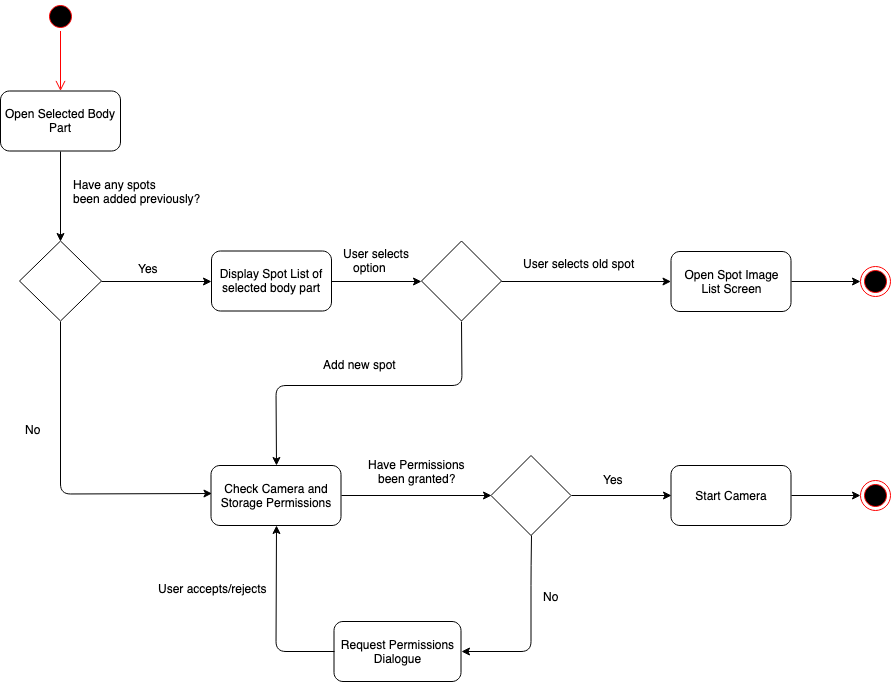
\includegraphics[width=1.2\textwidth, center]{figures/OldSpotList.png}
    \caption{UML Activity Diagram for the Old Spot's screen}
    \label{fig:OldSpotList}
\end{figure}

\subsection{Spot Image List}

This activity also extends the CameraOpeningActivity class, similarly to the \emph{OldSpotScreen}. This screen also makes use of the camera when a user elects to add a new photo of an existing spot. Figure \ref{fig:SpotImageList} depicts the process of the opening the screen, with the different paths available to the user. When the user opens the spot image list of a particular spot, all the photos of a spot are read from storage. This algorithm is displayed in Code Listing \ref{lst:loadingspotimages}. In a similar way to the algorithm in Code Listing \ref{lst:retrieveSpots}, spots are first loaded from storage with the \code{walk()} method. This creates a list of \code{imageFiles}, each of which we decode into an image path and thumbnail. We also initialise an array \code{selectedSpotBooleanList} to keep track of which images are being selected by the user (to compare).

Following the UML Diagram, the user can press the "+" button to add a new photo. If the goal is to compare two images, the user can either:
\begin{itemize}
    \item Press on an image for more than 2 seconds
    \item Click the "Compare" button on the toolbar
\end{itemize}
Both of these options would launch the \emph{Contextual Action Bar}, this is a toolbar that substitutes the default toolbar when a specific action takes place. It allows the user to select images from the list. If exactly two images are selected, a "Compare" button lights up, indicating the user can compare the images.

\begin{figure}
    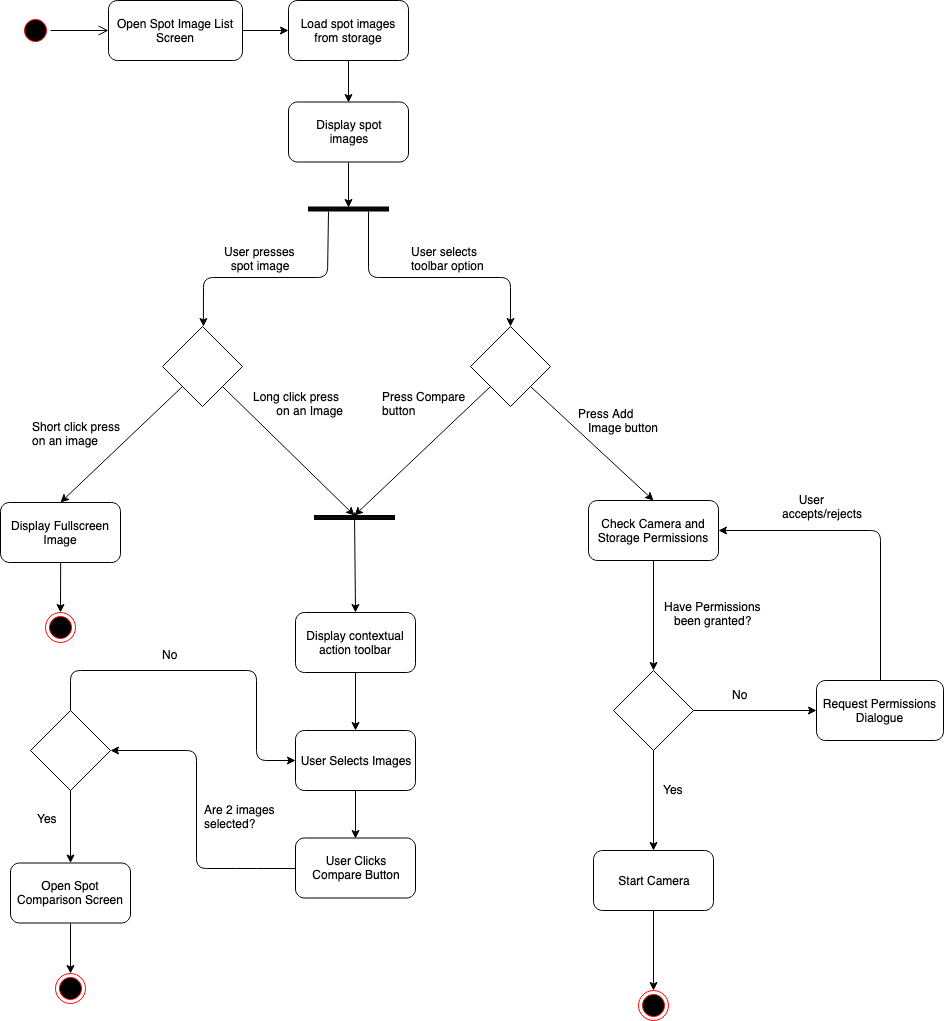
\includegraphics[width=1.2\textwidth, center]{figures/SpotImageList.png}
    \caption{UML Activity Diagram for the Spot Image List}
    \label{fig:SpotImageList}
\end{figure}
\begin{lstlisting}[caption={Loading spot images to compare}, label={lst:loadingspotimages}, language=Kotlin]
//Initialise arrays for each photo's path and thumbnails
var fullImagePaths = emptyArray<String>()
var imageThumbnails = emptyArray<Bitmap>()
//Loop through images in the selected spot's directory
val imageFiles =  File(spotDirectory).walk().maxDepth(1).toList()
for (i in 2..imageFiles.size) {
    fullImagePaths += imageFiles[i-1].toString()
    imageThumbnails += BitmapFactory.decodeFile(imageFiles[i-1].absolutePath)
}
numberOfImages = fullImagePaths.size
//Initialise dynamic array to keep track of which images are selected
val selectedSpotBooleanList = arrayOfNulls<Boolean>(fullImagePaths.size)
//By default, no images are selected 
Arrays.fill(selectedSpotBooleanList, java.lang.Boolean.FALSE)
\end{lstlisting}

\subsection{AddSpot Screen}

When the user chooses to add a new spot to a body part, they first take a photo, crop it to the desired dimensions, and is then redirected to this screen, the \emph{AddSpot} Activity. As shown in Figure \ref{fig:AddSpot}, they are asked to input a name for this spot, displaying appropriate error messages if the name violates any of the following properties:
\begin{itemize}
    \item Spot name is not left blank
    \item Spot name is under 20 characters
    \item Spot name contains only letters and numbers
\end{itemize}
This ensures stability when spot folders are created in storage, as any unrecognised characters (e.g. @, !, \$) could easily cause errors. The rules were devised following advice on folder naming conventions from \cite{santaguida_2011}. If the name satisfies these conditions, the spot folder is created in storage, substituting spaces for dashes ("-") to further comply with good practices.

The algorithm in charge of this task is shown in Code Listing \ref{lst:addSpot}. Running through the algorithm; a \code{photoDirectory} string is created, populating it by replacing the "temp" text with the body side, body part, and given spot name. This is the first step to move the image file from the temporary folder into a new folder named after the new spot. Next, a directory \code{newDir} is created at this path (making sure it doesn't exist yet through the \code{exists()} command). Once the folder is created, we proceed to move the image by modifying its path with the \code{renameTo} method. We then delete the (now empty) \code{tempfolder}, as the file has been successfully moved.

\begin{figure}
    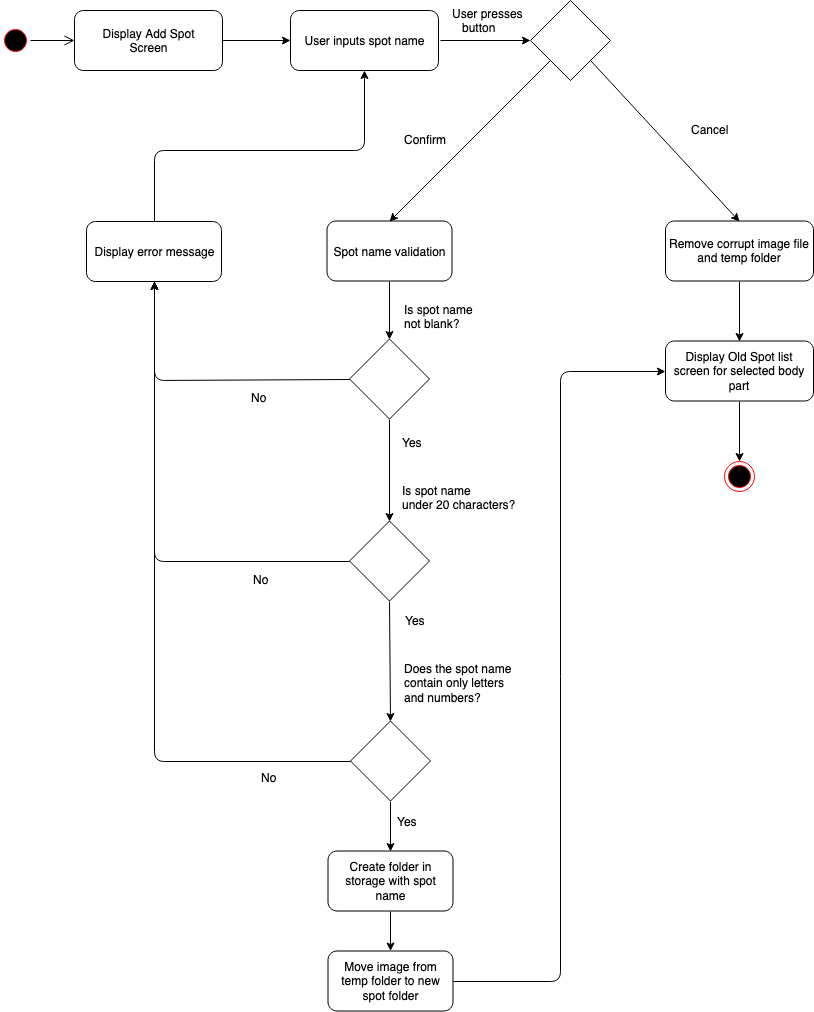
\includegraphics[width=1.2\textwidth, center]{figures/AddSpot.png}
    \caption{UML Activity Diagram for the \emph{AddSpot} Activity}
    \label{fig:AddSpot}
\end{figure}

\begin{lstlisting}[caption={Adding a Spot}, label={lst:addSpot}, language=Kotlin]
private fun moveImageFile(spotImageName: String, 
newSpotName: String, selectedBodySide: String, selectedBodyPart: String) {
    val photoDirectory = fullPhotoPath.removeSuffix(spotImageName)
    //Move image from temp folder to a new *newSpotName* folder
    val newDirPath = 
    photoDirectory.replace("temp", "$selectedBodySide/$selectedBodyPart/$newSpotName")
    val newDir = File(newDirPath)
    //Check if the directory exists already, create it otherwise
    if(!newDir.exists()) newDir.mkdirs()
    //Make app available in the device's Gallery
    Intent(Intent.ACTION_MEDIA_SCANNER_SCAN_FILE).also { mediaScanIntent ->
        val f = File(fullPhotoPath)
        mediaScanIntent.data = Uri.fromFile(f)
        sendBroadcast(mediaScanIntent)
        //Rename the file to the new path
        f.renameTo(File(newDirPath + spotImageName))
        //Delete the temporary folder
        val tempFolder = File(photoDirectory)
        deleteRecursive(tempFolder)
    }
}
\end{lstlisting}

\subsection{Compare Screen}
The workflow of the compare screen is very straightforward. Following the UML diagram in Figure \ref{fig:CompareScreen}, once the two images are displayed, the user's only options are to go back to the image list or email the two photos. If the user wanted to email the photos, they would press the email button, at which point the default email app is initiated, automatically creating a new message with the two attachments. Once the user sends the email, the compare screen opens again, displaying a \emph{Toast} message (short pop-up message that fades away after 2 seconds).

\begin{figure}
    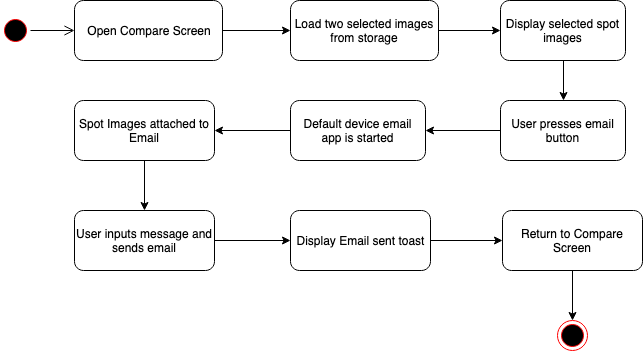
\includegraphics[width=1.2\textwidth, center]{figures/CompareScreen.png}
    \caption{UML Activity Diagram for the \emph{CompareScreen Activity}}
    \label{fig:CompareScreen}
\end{figure}

%If you outcomment then gotta explain
%\begin{lstlisting}[caption={Starting the comparison}, label={lst:startingcomparison}, language=Kotlin]
%//Initialise contextual action toolbar to allow user to select images
%mActionModeCallback = object : AbsListView.MultiChoiceModeListener { 
%    //This method is called whenever an item is selected or deselected
%    override fun onItemCheckedStateChanged(mode: ActionMode, 
%    position: Int, id: Long, checked: Boolean) {
%       //Update list of selected spots array
%        selectedSpotBooleanList[position] = checked
%        val checkedItemCount = listView.checkedItemCount
%        //Allow pressing the compare button if exactly 2 images are selected
%        mode.menu.findItem(R.id.compare).isEnabled = checkedItemCount == 2
%    }
%    //This method is called when the user presses a button in the
%    //contextual action toolbar.
%    override fun onActionItemClicked(mode: ActionMode, item: MenuItem): Boolean{
%        return when (item.itemId) {
%            //When the user presses the "compare" button
%            R.id.compare -> {
%                //Initialise array of indices of the images to compare
%                var spotIndicesToCompare = emptyArray<Int>()
%                //Loop through array of selected spots
%                (0 until selectedSpotBooleanList.size)
%                        //If a spot is selected, save it's index
%                        .filter { selectedSpotBooleanList[it]==true }
%                        .forEach { spotIndicesToCompare+= it }
%                //Get image paths for both spots to be compared
%                val firstSpotToCompare = fullImagePaths[spotIndicesToCompare[0]]
%                val secondSpotToCompare = fullImagePaths[spotIndicesToCompare[1]]
%                //Open the comparison screen and send info of selected sports
%                val intent = Intent(this@SpotImageList, CompareSpotScreen::class.java)
%                intent.putExtra("firstSpotToCompare", firstSpotToCompare)
%                intent.putExtra("secondSpotToCompare", secondSpotToCompare)
%                intent.putExtra("spotName", spotName)
%                intent.putExtra("spotDirectory", spotDirectory)
%                intent.putExtra("selectedBodyPart", selectedBodyPart)
%                intent.putExtra("selectedBodySide", selectedBodySide)
%                startActivity(intent)
%                //Return true if the click event has been handled
%                true
%            }
%            else -> false
%        }
%    }
%\end{lstlisting}

\section{Data Flow}
Most mobile applications require constantly sending information from one screen to another. This is done through the use of \emph{Intents}. In plain terms, an Intent is an intention to perform an action, or in other words, "a messaging object you can use to request an action from another app component" \cite{intents}. Intents can have data extras, these are key-value pairs such as strings or booleans. In the \emph{TrackYourSpot} context, the main data being attached to intents is:
\begin{itemize}
    \item \textbf{selectedBodySide} - "front" or "back"
    \item \textbf{selectedBodyPart} - "head", "back", "torso", "leftarm", "rightarm", "leftleg", "rightleg"
    \item \textbf{spotName} - User defined spot name such as "Spot1"
    \item \textbf{spotDirectory} - Directory of a spot in storage such as "/storage/emulated/0/Pictures/TrackYourSpot/front/torso/Spot1/"
    \item \textbf{spotListDirectory} - Directory of a body part in storage such as "/storage/emulated/0/Pictures/TrackYourSpot/back/head/"
    \item \textbf{spotImageName} - File name of a particular image such as "JPEG\_20190113\_133157.jpg"
    \item \textbf{fullPhotoPath} - Full path of an image such as "/storage/emulated/0/Pictures/TrackYourSpot/front/torso/Spot1/JPEG\_20190113\_133157.jpg"
\end{itemize}
An example intent can be found in Code Listing \ref{lst:intentdataflow}. In that particular example, the intent takes the user from the \emph{OldSpotList} to the \emph{AddSpot} screen. Note how variables and intent data labels are equal. This has been done to ensure consistency across screens and make sure it is clear what every variable represents in different screens.

\begin{lstlisting}[caption={Intent Dataflow for the \emph{AddSpot class}}, 
label={lst:intentdataflow}, language=Kotlin]
val intent = Intent(this, AddSpot::class.java)
intent.putExtra("selectedBodySide", selectedBodySide)
intent.putExtra("selectedBodyPart", selectedBodyPart)
intent.putExtra("spotListDirectory", spotListDirectory)
intent.putExtra("spotImageName", spotImageName)
intent.putExtra("fullPhotoPath", currentFullPhotoPath)
startActivity(intent)
\end{lstlisting}
\section{File Structure} \label{sec:filestructure}
The file structure for the app is relatively simple. Initially, images are stored in the default picture directory defined by each device. To identify this path, a File object needs to be created by calling the following method: \begin{verbatim}
getExternalStoragePublicDirectory(Environment.DIRECTORY_PICTURES)
\end{verbatim}
This file's path can then be identified by calling the inbuilt \code{getAbsolutePath()} method from the File.java class. 

\par Once we're located inside the absolute directory, pictures in .jpg format are saved in a \code{../bodySide/bodyPart/spotName}
folder hierarchy, where bodySide can be one of "front" or "back", bodyPart refers to the selected body part of a spot, it can take any of the following labels:
\begin{itemize}
    \item \textbf{Front} - head, torso, rightarm, leftarm, rightleg, leftleg
    \item \textbf{Back} - head, back, rightarm, leftarm, rightleg, leftleg
\end{itemize}
The spotName is the user defined name given to the spot at the time of adding the first image. Spot folders are created on demand, so the \code{../front/leftarm/worryingspot} folder will only be generated when the user takes a picture of a spot and gives it a name. Therefore, a typical folder structure could look like Figure~\ref{fig:filestructure.png}.
\begin{figure}
    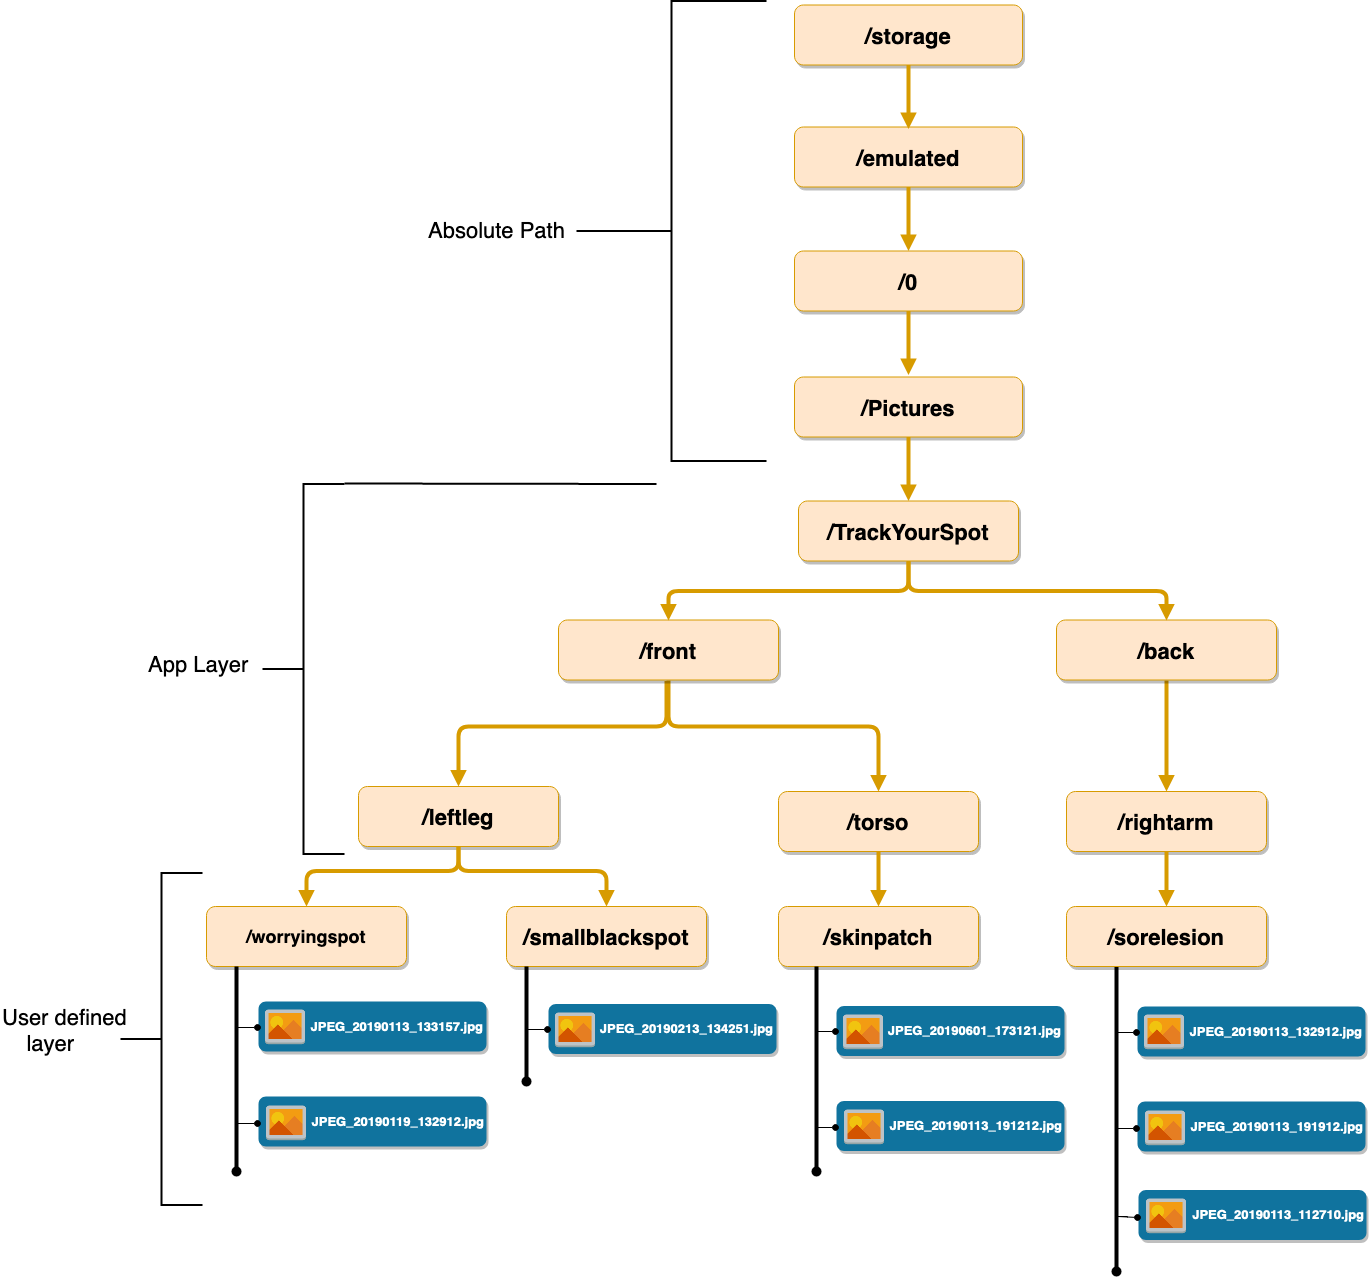
\includegraphics[width=1.2\textwidth, center]{figures/filestructure.png}
    \caption{A typical folder hierarchy showing folder layers within the user's device}
    \label{fig:filestructure.png}
\end{figure}
\par Another component of this file hierarchy are \code{/temp} folders. These temporary folders are only generated when pictures are not saved correctly due to the user closing the app without naming the spot, causing the spot to not be saved to the correct location.
\chapter{Deployment}
\section{Google Play Store}
This section will dive into the development and administrative tasks required to officially deploy the app to the public. This task only commenced once Beta Testing was declared complete. Recall the way we managed app releases through Alpha and Beta testing, deployment to production was done in a very similar way. The Android Developer Console facilitiated this task through a "Push to Production" button on the latest beta release of the app.
Before the app was pushed to production, a series of forms and administrative tasks were required. 

Firstly, an app title and descriptions were needed (Figure \ref{fig:appdetailsform}). These would be displayed on the app's download page, with the goal of persuading the user to click on the app and download it. After testing stages, it was decided to add the "Free Skin Cancer Tracker" label to the name. This is purely an advertisement instrument to ensure the app appears in as many searches as possible.

Secondly, the app's nature required the creation of a privacy policy (Figure \ref{fig:privacypolicy}). This is usually optional, but apps that require storage or camera permissions have to include one. An app privacy policy generator \cite{nishantsrivastava} was used for this task. The file was hosted on a \emph{Github} website repository to ensure it was permanently available.

Thirdly, the app's pricing details had to be defined (Figure \ref{fig:apppricing}). As determined previously, the app would follow a free business model, with no in app purchases or ads either. All 144 available countries would be included in the deployment list.

In fourth place, a content rating questionnaire had to be filled in (Figure \ref{fig:contentrating}). App content ratings intend to help parents identify potentially objectionable content that exists within an app. In the case of our app, the PEGI 3 age tag was delivered, this means Google determined the app to be suitable for all age groups.

Lastly, the app's graphics had to be uploaded (Figure \ref{fig:appscreenshots}). An app's graphics include:
\begin{itemize}
    \item App screenshots
    \item Highest resolution icon
    \item Feature graphic (banner)
\end{itemize}
The icon and banner were designed with the Inkscape vector graphics editor, combining different layers of copyright-free cliparts.

Once all the described forms were complete, the app was submitted to the Google Play Store. Four hours later, the app was successfully approved and officially deployed (Figure \ref{fig:applisting}). If you recall the app listing screenshot from Beta testing (Figure \ref{fig:betarelease}), the app title had an "(Unreleased)" tag. This tag is no longer shown.

\begin{figure}
    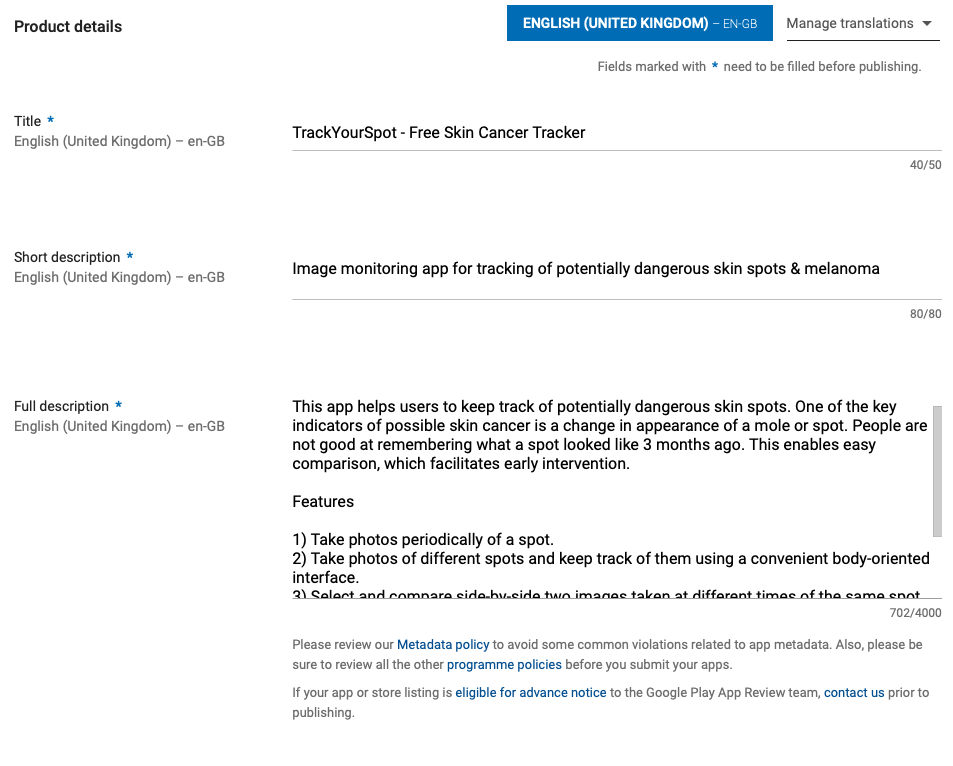
\includegraphics[width=1\textwidth, center]{figures/appnaming.png}
    \caption{Google Play Store App Details}
    \label{fig:appdetailsform}
\end{figure}

\begin{figure}
    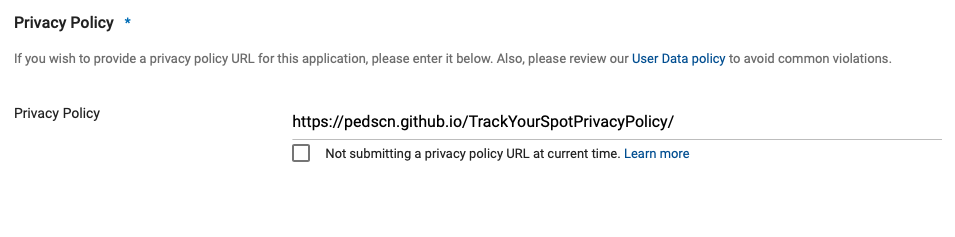
\includegraphics[width=1\textwidth, center]{figures/appprivacypolicy.png}
    \caption{Google Play Store Privacy Policy Form}
    \label{fig:privacypolicy}
\end{figure}

\begin{figure}
    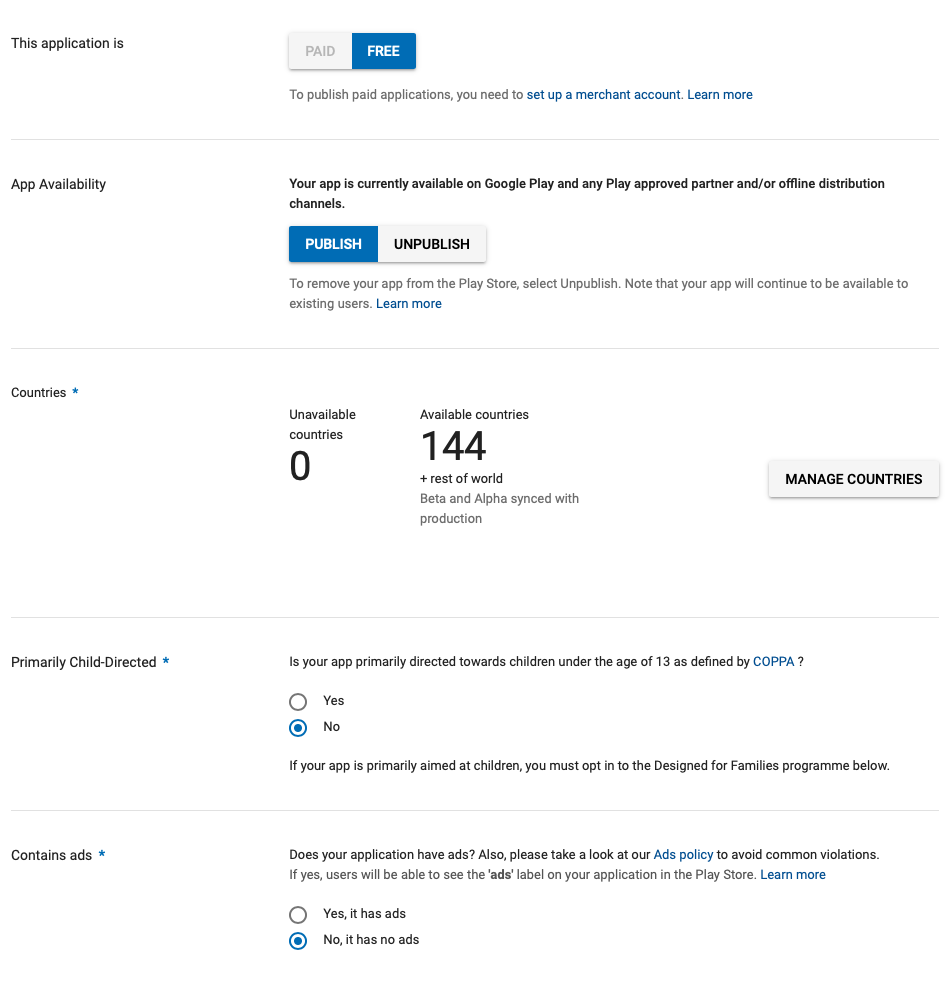
\includegraphics[width=1\textwidth, center]{figures/apppricing.png}
    \caption{\emph{TrackYourSpot} Deployment Settings}
    \label{fig:apppricing}
\end{figure}

\begin{figure}
    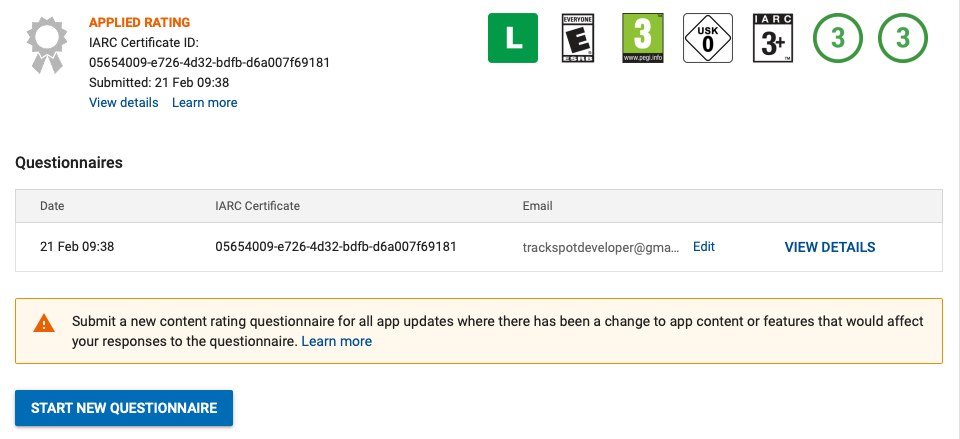
\includegraphics[width=1\textwidth, center]{figures/appcontentrating.png}
    \caption{Google Play Store Content Rating}
    \label{fig:contentrating}
\end{figure}

\begin{figure}
    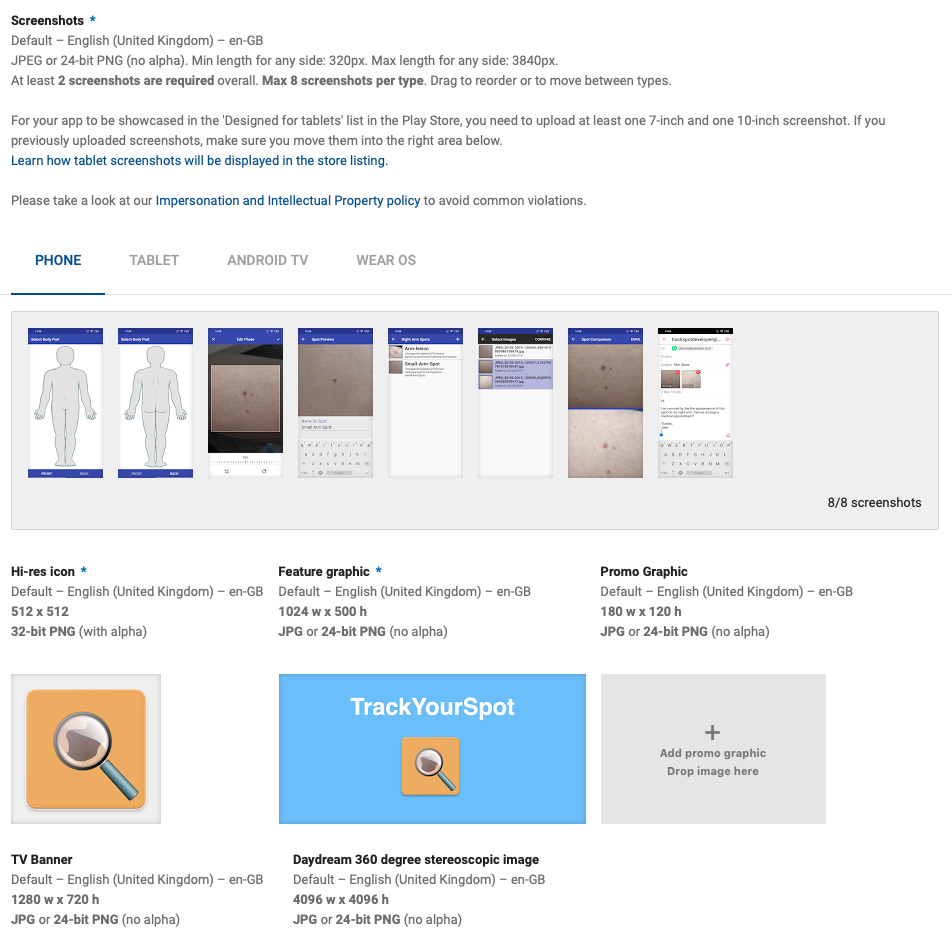
\includegraphics[width=1\textwidth, center]{figures/appscreenshots.png}
    \caption{Google Play Store Image Uploads}
    \label{fig:appscreenshots}
\end{figure}

\begin{figure}
    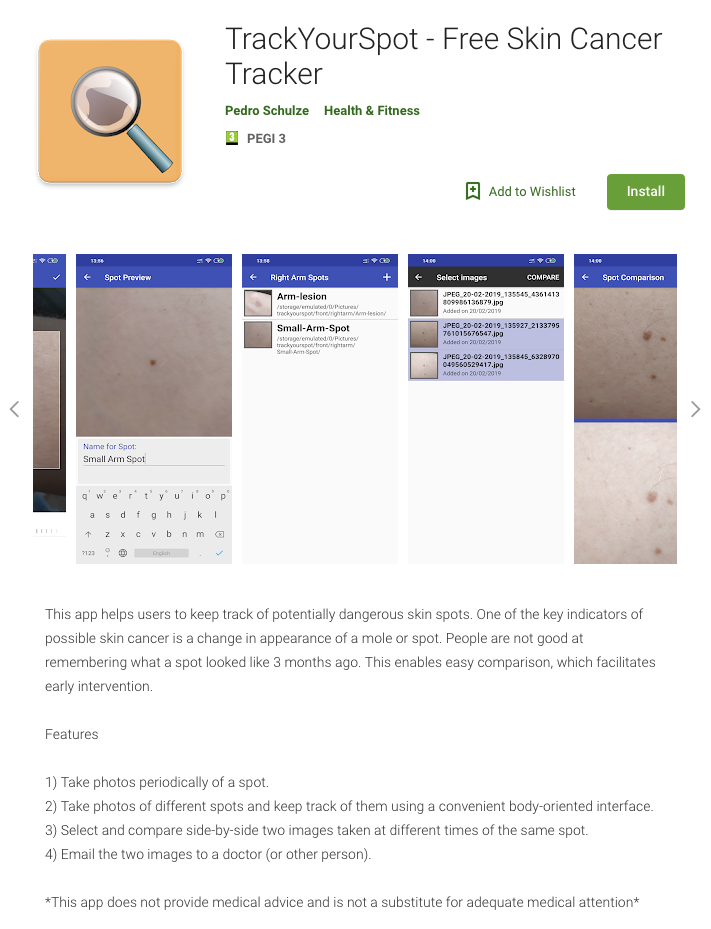
\includegraphics[width=1\textwidth, center]{figures/applisting.png}
    \caption{\emph{TrackYourSpot} app officially available to the public}
    \label{fig:applisting}
\end{figure}

\section{Website}
As part of the project, a website had to be developed to provide guidance on how to carry out all the core tasks of the app. To get started, a \emph{Bootstrap} business website template was downloaded from \emph{StartBootstrap} \cite{bootstrap}. Bootstrap is an HTML, CSS and Javascript framework to develop responsive websites \cite{twbs_2019}. This template was adapted to include links for all the tasks to be explained. Links for the Google Play Store and Android App Store versions of the app were also included. Figures \ref{fig:webdeployhome} - \ref{fig:webdeployadd} show a selection of screenshots of the finished website. The full website can be found at \code{www.trackyourspot.com}. 

This part of the project was also done by the iOS \emph{TrackYourSpot} developer, my contributions are described below: 
\begin{itemize}
    \item Page formatting and design of the home screen
    \item Finding suitable copyright free cliparts to be used as icons for the home screen (Figure \ref{fig:webdeployhome2}) 
    \item Modifying HTML code to describe steps to be completed for multiple tasks
    \item Attaching Android screenshots for each step
\end{itemize}


\begin{figure}
    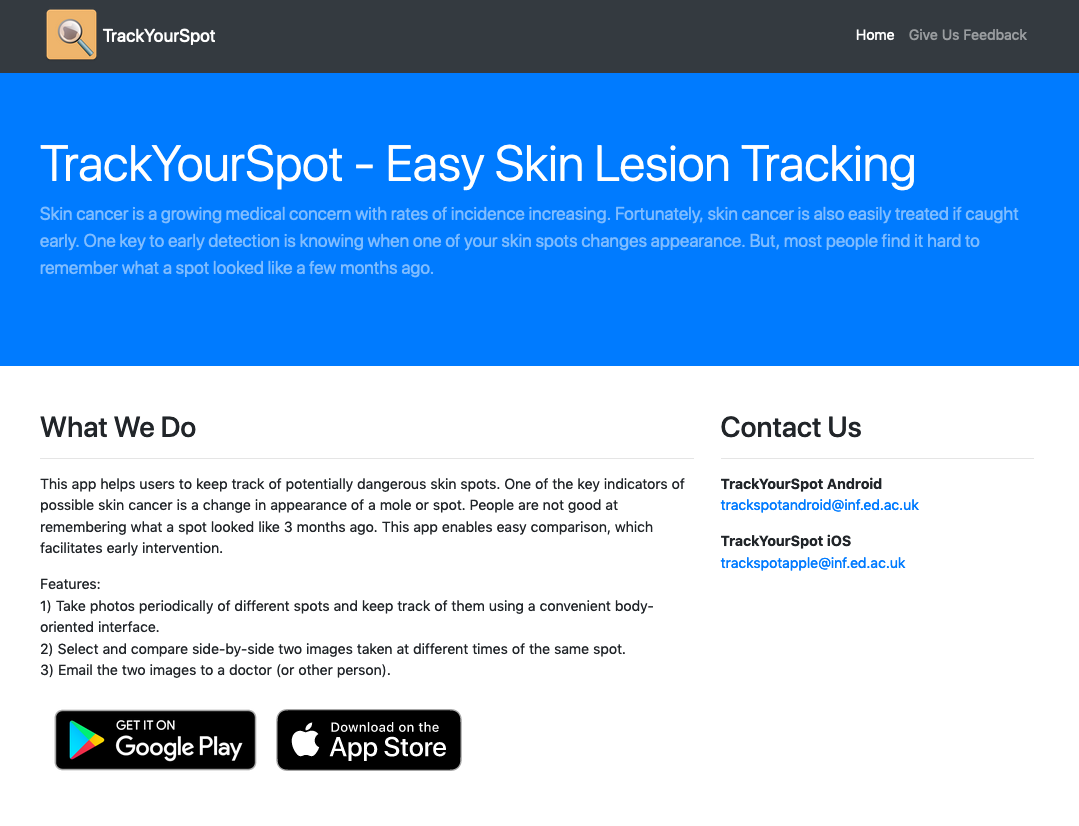
\includegraphics[width=1\textwidth, center]{figures/webdeployhome.png}
    \caption{\emph{TrackYourSpot} website homepage}
    \label{fig:webdeployhome}
\end{figure}

\begin{figure}
    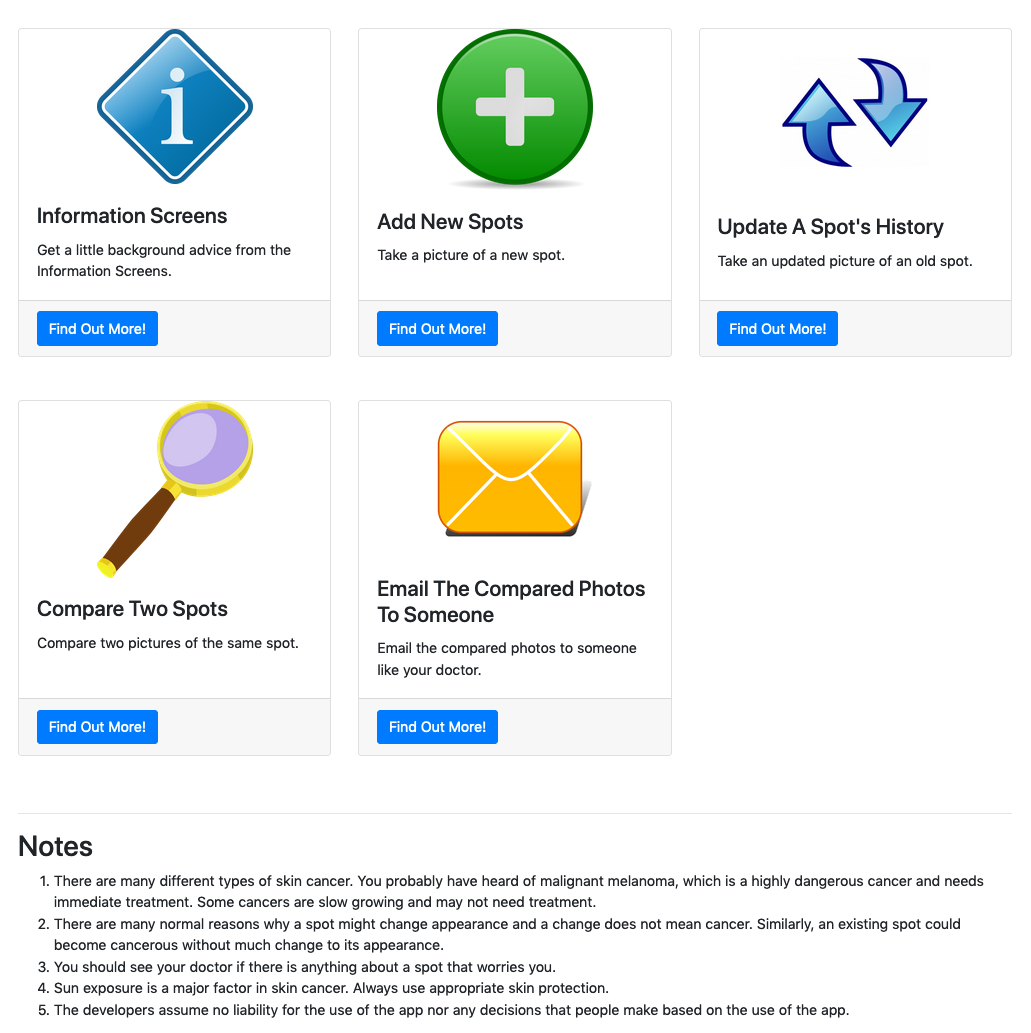
\includegraphics[width=1\textwidth, center]{figures/webdeployhome2.png}
    \caption{\emph{TrackYourSpot} website homepage (continued)}
    \label{fig:webdeployhome2}
\end{figure}

\begin{figure}
    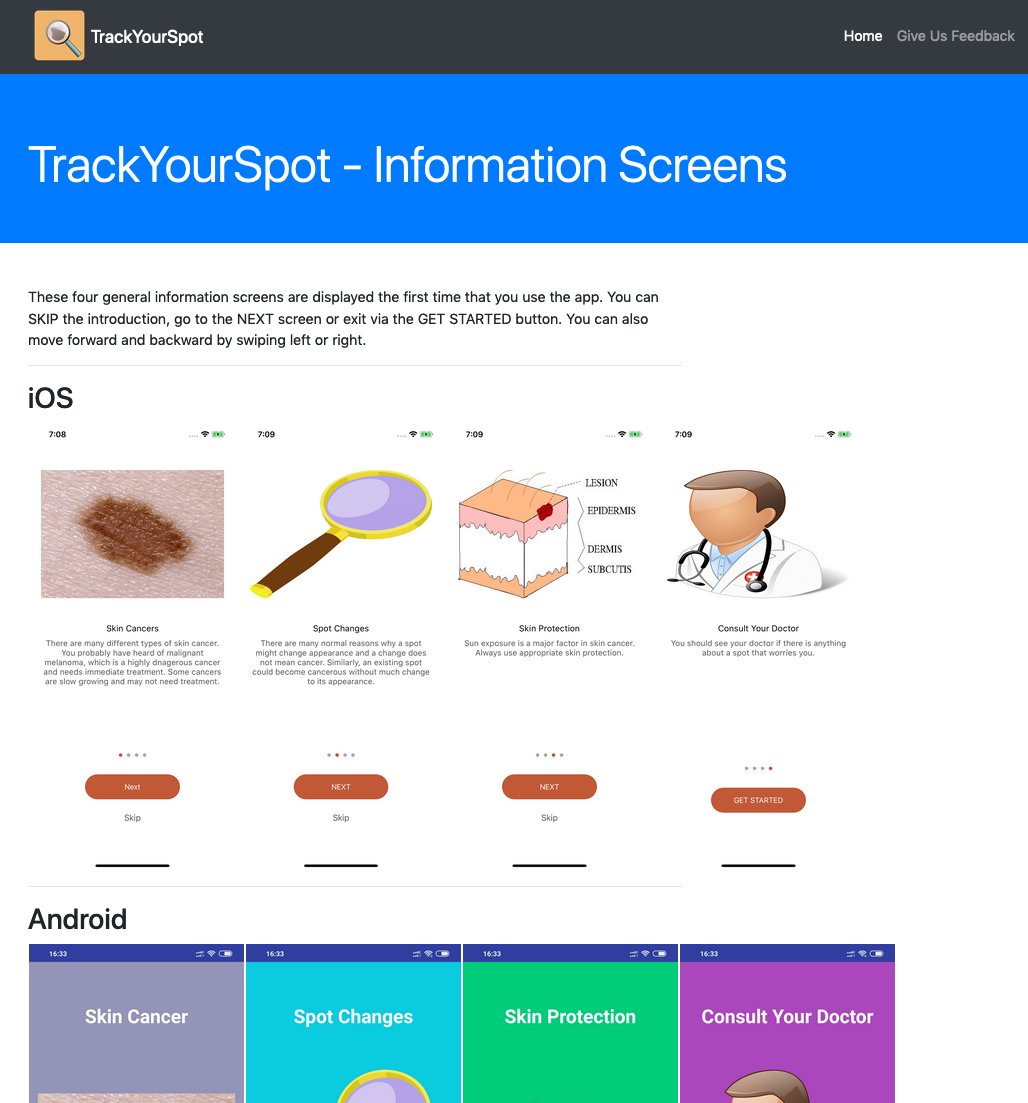
\includegraphics[width=1\textwidth, center]{figures/webdeployinfo.png}
    \caption{\emph{TrackYourSpot} website information screens guidance}
    \label{fig:webdeployinfo}
\end{figure}

\begin{figure}
    \includegraphics[width=1\textwidth, center]{figures/webdeployadd.png}
    \caption{\emph{TrackYourSpot} website adding a spot guidance}
    \label{fig:webdeployadd}
\end{figure}



\chapter{Testing and Evaluation}
Testing of the app was carried out in four main stages. Including both technical functionality tests and user design evaluations. They can be summarised into the following:
\begin{itemize}
    \item \textbf{Internal Testing} - Also known as "pre-alpha", this stage was carried out for both major and minor bug fixes. It prepared the app to be further tested by external testers.
    \item \textbf{User Acceptance Testing} - This stage was used for minor bug fixes. The app was exposed to users in a controlled, private circle (alpha testers) and later to the general public in the beta stage.
    \item \textbf{Preference Testing} - This stage took place by surveying users on their preferred interface between two different design concepts for multiple screens in the app.
    \item \textbf{Usability Evaluation} - Usability testing involved assessing the user experience through both qualitative and quantitative measures. These included interviews, think-aloud sessions and system usability scale reports.
\end{itemize}

\section{Internal Testing}
Once the final stages of development were completed, the internal testing phase commenced. Internal testing's main focus was around testing multiple SDK versions and particularly the minimum SDK at which the app remains stable. Other areas of focus involved testing the appearance of the UI accross different screen sizes and resolutions. This testing stage helped set up for the larger scale alpha and beta tests, as we could get a good idea of the device range we were targeting and it ensured the core features of the app were fully functional and accessible. Internal Testing took place across 10 different devices, ranging between physical devices and emulators. Table \ref{devicetable} shows the list of devices and operating systems that were tested at this stage:
\begin{table}[ht]
\centering
\begin{tabular}{|l|}
\hline
Xiaomi Pocophone F1 - API 28 (Pie)                       \\ \hline
Motorola Moto E - API 19 (KitKat)                        \\ \hline
Xiaomi Mi Max 2 - API 25 (Nougat)                        \\ \hline
Lenovo Zuk Z1 - API 23 (Marshmallow)                     \\ \hline
Google Pixel - API 21 (Lollipop)                         \\ \hline
Google Pixel - API 19 (KitKat)                           \\ \hline
Nexus 6 - API 21 (KitKat)                                \\ \hline
Nexus 6 - API 21 (Lollipop)                              \\ \hline
3.7 inch FWVGA display slider emulator - API 25 (Nougat) \\ \hline
Nexus S - API 23 (Marshmallow)                           \\ \hline
\end{tabular}
\caption{Table of devices and operating systems used for testing}
\label{devicetable}
\end{table}
\par

\begin{figure}
    \includegraphics[width=1\textwidth, center]{figures/4devicestesting.jpg}
    \caption{\emph{TrackYourSpot} app being tested accross different devices}
    \label{fig:4devicestesting}
\end{figure}

As seen by Figure \ref{fig:4devicestesting}, the screen sizes vary from 3.7 inches to 6.4 inches, with resolutions from 540 x 960 pixels to 1080 x 2246 pixels. This gives us a perfect range to assess how the UI adapts to different screens. This revealed a bug where small screens (smaller than 4 inches) did not display the left and right leg buttons. This was due to incorrect layout constraints in the XML file for the Body Screen. The app was also tested across different versions of the Android platform. Any new Application project on Android Studio will by default target the latest Android SDK and, as of this moment, have a minimum SDK of 23 (Marshmallow). It is the developer's job to decide whether this minimum SDK version should be lowered or not, depending on compatibility issues of APIs used in the application. Without adequate testing of SDK versions, some users would be able to download the app with risk of crashes and malfunctioning.
\par After multiple tests progressively lowering the SDK version, it was observed that issues started to arise with the KitKat operating system. This was expected, as the Android update documentations for APIs 19 and 21 clearly state behaviour changes for Permissions \cite{androiddevelopers}, reading from storage, or bitmap handling \cite{androiddevelopers2} . All of which are done within the app. The CameraOpeningActivity() classes were crashing due to a multitude of problems with Camera/Storage permissions, Intent data flows and File URI's. Some of these issues could be fixed by adding a simple if statement checking the current Android version of the device, for example:
\begin{lstlisting}[caption={Checking the Android Build Version}, label={lst:checkAndroidVersion}, language=Kotlin]
if (Build.VERSION.SDK_INT >= Build.VERSION_CODES.LOLLIPOP) {
    takePictureIntent.addFlags
    (Intent.FLAG_GRANT_WRITE_URI_PERMISSION)
} else {
    val clip = ClipData.newUri(contentResolver, "clipData", photoURI)
    takePictureIntent.clipData = clip
    takePictureIntent.addFlags(Intent.FLAG_GRANT_WRITE_URI_PERMISSION)
}
\end{lstlisting}
These workarounds made the app stable in some API 19 devices, such as the Google Pixel, however other same OS devices would still run into crashes, and hence it would be unwise to make the app available for these. Under less time constraints, it would be ideal to improve support for older Android versions, however as shown by Google in their publicly available distribution dashboard (Figure \ref{fig:Androidversionstats.png}). Devices with API's under 21 only account for 11.1\% of all devices, meaning our app is still available for almost 90\% of devices. At this point it was decided to set the minimumSDK to 21, and focus on other areas of the project. However, as the app's main user base will not have have up to date Android versions, the usage stats will determine whether developing the apps compatibility becomes a priority again.
\begin{figure}
    \includegraphics[width=1.2\textwidth, center]{figures/Androidversionstats.png}
    \caption{Android Device Distribution of Platforms}
    \label{fig:Androidversionstats.png}
\end{figure}
\section{User Acceptance Testing}
User acceptance can be defined as the last stage of the software testing process. At this stage, the app is exposed to real end-users. The two test stages in User Acceptance Testing were:
\begin{enumerate}
    \item Alpha Testing
    \item Beta Testing
\end{enumerate}
These tests were smoothly supported by Google's Android Developer Console platform, allowing for easy deployment from one to another and user friendly controls to manipulate these. The two sections below will delve into the details of these, describing bugs and issues that arised in the process.
\subsection{Alpha Testing}
After the app was confirmed to be stable accross the range of Android versions and screen sizes in the internal testing stage, the app was published on the Google Play Store under a private url (Figure \ref{fig:alpha_testers.png}).
\begin{figure}[H]
    \includegraphics[width=1.2\textwidth, center]{figures/alpha_testers.png}
    \caption{Alpha Testing Tester selection, feedback channel and download URL}
    \label{fig:alpha_testers.png}
\end{figure}
Any testers could be simply added to the tester mailing list and sent the url to the \emph{TrackYourSpot} application to download on their devices. As Google Play Developer's console dictated, all testers were required to have gmail accounts, somewhat limiting the scale at which alpha testing could be carried out. Despite this limitation, 14 testers were selected throughout alpha testing. The group was mainly composed of penultimate and final year Computer Science students at The University of Edinburgh.
\par It was clear that the testers's background and computer literacy would be ideal to spot any hidden or convoluted bugs that escaped Internal testing. This resulted in many small fixes and 11 updates (Figure \ref{fig:alpha_releases.png})
\begin{figure}
    \includegraphics[width=1.2\textwidth, center]{figures/alpha_releases.png}
    \caption{Alpha Release APK list}
    \label{fig:alpha_releases.png}
\end{figure}
during the 2 weeks of alpha testing. The main functionality bugs encountered were: \todo{expand on these}
\begin{itemize}
    \item temp folder removal
    \item Closing camera or cropping screen midway
    \item Empty app crash, thumbnail 
    \item automatically open camera
\end{itemize}
\par This stage started to reveal some UI issues that could become problematic at Beta or production level. This was to be expected, as the app's reach had substantially expanded to outside the developer's eyes. The following UI issues were discovered: \todo{expand}
\begin{itemize}
    \item Lack of Information Screens
    \item Lack of Compare button
\end{itemize}

\subsection{Beta Testing}
Once alpha stage was complete, an app release was pushed to the beta stage. This proved to be a significant milestone for the project, as in an Android application development context, the app was now fully available to the public. Android apps in beta stage are fully available to everyone (likewise to a production-level finished app), with the difference of the app having an "Unreleased" tag next to its name (Figure \ref{fig:betarelease}) and the user being able to send direct feedback to the developer. This meant the app was now ready and fully available for anyone and the project would be able to receive feedback and reviews from anonymous people. 

\begin{figure}[H]
    \includegraphics[width=1.2\textwidth, center]{figures/betarelease.png}
    \caption{Google Play Store's display of \emph{TrackYourSpot} in Beta testing}
    \label{fig:betarelease}
\end{figure}

Before this point, it was crucial to properly execute both the internal and alpha testing stages, as any significant bugs or incompatibilities would have been disastrous at these early stages of an app's release. As described by \cite{joorabchi2013real}, "If users like an app, they download and start using it. If not, they delete it and move on immediately. If they really like it, they rank it high; Or if they really dislike it, they go on social media and complain. Thus, a low-quality release can have devastating consequences for mobile developers.". This quote refers to the official release of an app, but Android's user ratings are available since the beta release, and hence this milestone carries an equal responsibility.

Issues discovered during beta stage include: \todo{expand}
\begin{itemize}
    \item Deleting spot folders
    \item Information screen text overflowing
    \item Body label name spelling
    \item Repeating names of body spots
\end{itemize}

\section{Preference Testing}
An initial plan was made to carry out \emph{A/B Testing} with multiple app design options. The process can be defined as randomly assigning users into segments, displaying a different design variant to each and comparing them based on "Metrics of interest, ranging from runtime performance to implicit and explicit user behaviors and survey data" \cite{kohavi2009controlled}. This could be neatly done in parallel with the think-aloud study, however, as the project developed, it was clear that there were limitations and constraints to taking this approach:
\begin{itemize}
    \item \textbf{Nature of design screens being assessed} - The main design features being assessed were trivial visual or appearance changes on a single screen. These ranged from a choice of colours to button visibility and/or position. If the design decisions being assessed significantly changed how a core task is carried out, such as adding or comparing a spot, then completing A/B tests would make more sense.
    \item \textbf{Response sample size} - Due to the limited availability of elderly candidates (Over 50 years old) for the think aloud study, the results for design choices would be more biased towards the younger users which were participating in the study, therefore not giving an accurate representation of the superior design in the eyes of more realistic end users (older individuals).
\end{itemize}
The factors above suggested that trading part of the study's formality for more plentiful results and statistics would be beneficial. This incited to take a more general approach, arriving at the concept of \emph{Preference Testing}. In psychology, a preference test can be defined as an analysis where consumers are asked to express a preference between rival products \cite{m.s._2015}. In the area of software design, we can translate it to presenting users with multiple visual designs to determine which one they prefer and why. This was done through the method of an online questionnaire. Reasons for this include:
\begin{itemize}
    \item \textbf{Statistics Analysis} - Availability of predefined statistics visualization, filtering, and analysis tools for design preference questions. A straightforward comparison of designs can be done by measuring preference votes. 
    \item \textbf{Time and Participation Numbers} - Once the survey's final version was complete, it was evidently easy to share and collect responses. The survey would take 2 minutes to complete and ensure that a much higher volume of opinions was collected.
    \item \textbf{Qualitative Feedback} - Allowing for both open ended and inclusion of demographic questions would provide useful data in terms of why users prefer design A/B.
\end{itemize}
The questionnaire form can be found in Appendix A. The choice of questions had been carefully chosen after an initial pilot survey had been designed. This initial design was lacking background information on the project. In addition, the questions weren't always clear and often had ambiguous choices or answers. The reliability of the survey was evaluated, putting particular emphasis on whether the questions being asked were actually understood, following the advice of using very simple language and avoiding little-known words \cite{gendall1998framework}. Open ended questions were kept to a minimum and Likert-type answer scales \cite{boone2012analyzing} were used.

\subsection{Results}
The survey was circulated through the 4th year undergraduate Informatics group, varied groups on social networks and friends and family of everyone involved in the project. As a result, a total of 46 responses were collected. Figures \ref{fig:surveyresult1} - \ref{fig:surveyresult8} show answers to both demographic and design questions in different charts. We can analyse the results below:
\begin{enumerate}
    \item \textbf{Please specify your age}
    \\ Over 2/3 of the survey participants were between the ages of 18 and 30. This is far from ideal, as the app's target audience is the middle-aged to older population. One of the biggest challenges of the project's testing and evaluation stage was collecting data from older users. This is clearly shown by this data. Nonetheless, 32.61\% of the responses were from people over the age of 30. This combination of figures should provide some interesting answers to the rest of the survey and make an attempt at balancing answers across all age groups. 
    \item \textbf{Please specify your gender}
    \\ More than 3/4 of the answers came from the male gender, this had to be expected when the survey was circulated through a university group with male dominated demographics. However, this turned out to be an advantage for the study, as according to research by \cite{fisher2013disproportionate}, "men are 55 percent more likely to die of melanoma than women" between the ages of 15-39, converting the answers of male individuals in that age group into very valuable participants for the study.
    \item \textbf{What smartphone operating system do you regularly use?}
    \\ 56.52\% of users are regular iPhone users and 43.48\% use Android. As the two clearly dominating operating systems in the market, this is completely expected. These stats don't mean much on their own but they will become useful to understand the design preferences of users, for example iPhone users might dislike more Android specific designs and viceversa.
    \item \textbf{What do you consider the most important in app design? (Tick all that apply)}
    \\ This question acts as a build up to help in understanding the results of questions 6-7. "Ease of Use" was the most popular option, with over 80\% of participants including it on their list of preferences. At 65\% and 63\%, we have "Clean look" and "Intuitiveness". On the other side, "Colors and Patterns" and "Text and button size" seem to be less important to users, being only selected 18\% and 24\% of the time. This should allow for good predictions on what design users will prefer in questions 6 and 7.
    \item \textbf{How likely are you to use an app to monitor your skin spots?}
    \\ over 58\% of participants claim they are unlikely or very unlikely to use this kind of app. These numbers do seem a bit low, however most likely expected from a group of mainly 20-25 year old student. Looking back, the phrasing of the question could have been improved by adding "in the future", since it is likely that some participants wouldn't use it at this point in time, but more likely in the future. Another option would be to rephrase the question to "How likely are you to recommend this app to an elderly relative?", since it would provide better feedback on whether the concept and design of the app are adequate. 
    \item \textbf{Rank these 4 designs from best to worst (Best=1, Worst=4)}
    \\ Looking at the 4 designs being assessed (Appendix A), users seemed to rank Design C as the best over 52\% of the time, this makes it a clear favourite compared to Design D, which was only voted as the favourite 26\% of the time. Designs A and B performed worse, being only voted as the favourite 10.87\% of the time. It is worth noting that designs A and B seemed to be popular second choices, with 31\% and 33\% frequencies. Analysing the designs, the popularity of Design C seems logical with respect to the answers to question 4. Most users preferred a clean and intuitive look, while dismissing the need of labelled buttons.
    \item \textbf{Which of the two designs (A or B) would you prefer using?}
    \\ The results to this question were the least expected, over 80\% of participants preferred Design B over A (see Appendix A). The design in A tries to emulate official Android design guidelines, displaying an action float button. Design B is closer to iOS guidelines, displaying the button on the right corner of the toolbar. Knowing around 57\% of users are iPhone users (Question 3 results), it was predicted that design B would come out slightly on top. With the clear popularity of design A, it is obvious that replacing the "+" button on the toolbar with a floating action button is the right choice.
    \item \textbf{Do you have any comments about these designs or the concept of the app?}
    \\ Figure \ref{fig:surveyresult8} shows a few responses that participants provided for this question. Overall, the feedback was very useful, most of which can be used to further improve the app's design. A few interesting ideas people suggested include:
    \begin{itemize}
        \item Pick better color schemes for the body images, also altering the opacity
        \item Let users choose the exact position of a skin spot
        \item Increase the size of the toolbar buttons
        \item Display a dialogue if no spots have been added
    \end{itemize}
\end{enumerate}
\clearpage
\begin{figure}[H]
    \includegraphics[height=10cm, center]{figures/surveyresult1}
    \caption{Question 1 results of the Preference Testing Survey}
    \label{fig:surveyresult1}
\end{figure}
\begin{figure}[H]
    \includegraphics[height=10cm, center]{figures/surveyresult2}
    \caption{Question 2 results of the Preference Testing Survey}
    \label{fig:surveyresult2}
\end{figure}
\begin{figure}[H]
    \includegraphics[height=10cm, center]{figures/surveyresult3}
    \caption{Question 3 results of the Preference Testing Survey}
    \label{fig:surveyresult3}
\end{figure}
\begin{figure}[H]
    \includegraphics[height=10cm, center]{figures/surveyresult4}
    \caption{Question 4 results of the Preference Testing Survey}
    \label{fig:surveyresult4}
\end{figure}
\begin{figure}[H]
    \includegraphics[height=10cm, center]{figures/surveyresult5}
    \caption{Question 5 results of the Preference Testing Survey}
    \label{fig:surveyresult5}
\end{figure}
\begin{figure}[H]
    \includegraphics[height=10cm, center]{figures/surveyresult6}
    \caption{Question 6 results of the Preference Testing Survey}
    \label{fig:surveyresult6}
\end{figure}
\begin{figure}[H]
    \includegraphics[height=10cm, center]{figures/surveyresult7}
    \caption{Question 7 results of the Preference Testing Survey}
    \label{fig:surveyresult7}
\end{figure}
\begin{figure}[H]
    \includegraphics[height=10cm, center]{figures/surveyresult8}
    \caption{Question 8 results of the Preference Testing Survey}
    \label{fig:surveyresult8}
\end{figure}

\section{Usability Evaluation}
The evaluation of the app's user design and experience was carried out through a series of popular methodologies in UI evaluation. Three usability studies were carried out, with the goal of revealing problems that would go unrealised with a single usability evaluation \cite{article}. Prof. Tselios' findings declare that the value of combining usability studies lies on providing "different but synergistic perspectives on various aspects of the user interface". While this claim is based on evaluating educational applications, one would assume this translates to most design evaluations. The three studies performed were:
\begin{itemize}
    \item Think-Aloud
    \item System Usability Scale Evaluation
    \item Interviews
\end{itemize}
The individual studies are explained in-depth below. The justification and execution of these is emphasized, with the results of all three studies summarized at the end of the section.
\subsection{Think-Aloud Sessions}
The chosen study was a \emph{Concurrent Think-aloud}, where users are asked to walk through tasks and and articulate what they are doing, as opposed to a  \emph{Restrospective Think-aloud}, where they complete the tasks in silence while being recorded \cite{hanington2012universal}. The main problems with the concurrent think-aloud approach are:
\begin{itemize}
    \item \textbf{Unnatural feeling} - Thinking aloud while using an app often seems unnatural for users. This means they will often unconsciously leave some thoughts out, making it impossible to know everything that goes through the user's mind \cite{rubin1996handbook}.
    \item \textbf{Lack of quantitative measures} - Asking users to think aloud while using the app significantly slows down the process, making it useless to measure variables such as time taken on task. The useful data that can be collected from this study revolves around \emph{where} and \emph{why} problems exist.
\end{itemize}
Despite these drawbacks, the choice of this study can be justified in several ways. Firstly, the low cost of the study, as only a notepad and an Android device are needed. Secondly, a low number of participants will usually highlight most of the issues with the design being evaluated. Thirdly, the tasks being assessed were considered to be of easy-intermediate difficulty. As denoted by \cite{charters2003use}, think-aloud studies should be done with systems that require "more than an automatic response but should not be cognitively overwhelming.", hence suggesting think-aloud to be appropriate for this project.

Before the study could commence, an ethics review of the study had to be submitted to the school's ethics board. Once approval was granted, participants were asked if they would like to take part in the study. Each of them would then have to agree to sign a consent form, they would also be shown an information sheet before they started the study (See Appendices B and C). The think-aloud script was then read to participants. Subsequently, they were asked to carry out these four tasks one step at a time:
\begin{enumerate}
    \item Add a new spot in your \textbf{front right arm}. Give it the name "Small spot"
    \item Add a new image to the previously created spot "Small spot"
    \item Compare two images of the previously added "Small spot".
    \item Without exiting the \emph{TrackYourSpot} app, email two images of the previously added "Small spot" to the following address: trackspotandroid@gmail.com
\end{enumerate}
While carrying out these tasks, the device's sound recorded app was used in the background, this allowed for audio files to be revisited at a later stage. Participants were constantly reminded to talk out loud, while the researcher took notes of their comments and behaviour. The researcher was not allowed to answer any questions and the participant had to decide when they believed a task was complete. Each instance of the study would take between 20-30 minutes on average.

\subsection{System Usability Scale}
To achieve a quantitative measure of usability for the app, the \emph{System Usability Scale} was used. As John Brooke describes it \cite{brooke1996sus}, it is "robust and reliable", and a powerful evaluation tool that "correlates well with other subjective measures of usability". The SUS form used in question can be found in Appendix D. This form was presented to participants after their participation on the think-aloud study. The effectiveness of this evaluation method relies on the participant having fresh memory of the tasks and features of the app.

Once every participant completes the form, a score is calculated between 0-100. Even numbered questions receive a value of 5 minus the scale position, odd numbered questions are simply the scale position minus 1. The sum of these scores multiplied by 2.5 returns the SUS Score.

While the SUS evaluation system has been widely used for a variety of research projects, its effectiveness can still be criticised, particularly when applied to projects such as this one. These issues could be:
\begin{itemize}
    \item \textbf{Lack of Adaptability} - While the form's questions can generally be modified and adapted to your project, it is not clear whether the changes will alter the validity of the SUS score, weighting system, or the overall study.
    \item \textbf{Imprecise Terms} - Statements such as \emph{I would like to use the system frequently} or \emph{needed to learn a lot} can have different meanings to different users. In addition, an average app would consider usage of once a month an infrequent time frame, however, for a skin spot monitoring app, this would be very frequent.
    \item \textbf{Simple Language} - Terms such as "cumbersome" or "various functions in the system were well integrated" were used in the form. As a general rule, technical terms should be avoided and language used should be easily understood by users with no technical knowledge \cite{harrison2007tip}.
\end{itemize}

\subsection{Interviews}
Following the completion of the SUS form, users were asked a series of interview questions about the overall usability of the app. Typically, one of \emph{Interviews} or \emph{Focus Groups} is used as a qualitative measure of usability. Following the decision to carry out think-aloud studies, performing interviews seemed like the obvious choice. Their flexibility and ability to be used together with other evaluation methods was worthwhile. Performing interviews after another usability activity allows to better understand the issues and results in depth \cite{courage2005understanding}.
The following five questions were asked:
\begin{enumerate}
    \item Which tasks did you find particularly easy to follow?
    \item Which tasks did you find more challenging?
    \item Are there any changes you would make to the design of the app?
    \item Was the website useful in helping you learn how to use the app?
    \item Did you find the information displayed on the information screens relevant?
\end{enumerate}
The interview followed a \emph{semi-structured} type design, where the set of questions above were used as a starting point. Followup questions and deviations were made frequently whenever participants mentioned an interesting idea or concern. Answers to questions were also recorded and written notes were made when appropriate.

\subsection{Results}
A total of 9 participants agreed to take part in the study. The feedback collected from the first few participants was particularly insightful, after that, the value of the study started diminishing as users started to point out the same issues over and over again. At this point, it was decided to not continue the study, but perhaps repeat it in the future once the issues have been addressed. All 9 participants agreed to take part in the study. This involved signing the consent form, participating in the Think-Aloud and Interview stages, and finally filling in the System Usability Scale Form. We will analyse the results of these studies individually.

In the case of the Think Aloud study, the analysis of the data was done by listening to the recordings and reviewing the notes taken at each experiment. Both of these were analyzed to determine if there were any patterns in how users interacted with the app. This consisted of the problems where users got stuck on or how they went about solving problems. The main issues highlighted for each task were:
\begin{enumerate}
    \item \textbf{Add a new spot in your front right arm. Give it the name "Small spot"}
    \\ Users found this task relatively straightforward, they clicked on the right arm straight away, proceeded to take a photo of a spot and crop it, knowing that they had completed the task when returning to the main menu. Occasionally the participant would add the button to the back "Right Arm" instead, quickly realising they hadn't paid enough attention to the task. Participants commented on the clarity of the UI while completing this task. As a small issue, some participants appeared to not zoom in enough when cropping the photo, this would make the spot harder to inspect when comparing it on task 4.
    \item \textbf{Add a new image to the previously created spot "Small spot"}
    \\ This task was completed with more difficulties than the previous one. The most common mistake was participants adding a completely new spot to the right arm instead of adding a new photo to the existing spot. Participants showed difficulty in realising the "Small spot" list item represented a folder that could be clicked on, instead assuming it was simply an image. Some users realised their mistake when trying to complete the next task, as they weren't able to compare two separate spots. It was also pointed out that the button for adding a new photo looked too similar to the button for adding a new spot, implying these should be clearly differentiable.
    \item \textbf{Compare two images of the previously added "Small spot".}
    \\ The success of this task was very dependent on whether task 2 was carried out correctly, the participants that added the 2 photos correctly usually had no issues comparing them. Some participants realised they had to add another photo to be able to compare, and 1 participant required guidance to be able to complete the task. Another participant thought opening the images individually and swiping left and right was enough to compare them, and declared the task finished before actually comparing them side by side. Most participants pointed out that the compare screen was missing an option to zoom in to the images, this was particularly the case when they didn't crop the images to an adequate zoom. This suggests there could be better guidance on how to take photos. 
    \item \textbf{Without exiting the TrackYourSpot app, email two images of the previously added "Small spot" to the following address: trackspotandroid@gmail.com}
    \\ Compared to the other tasks, this task was completed very easily, users spotted the "Email" button on the compare screen straight away and proceeded to email both photos to the address. A few participants pointed out the lack of a dialogue message to know if the email has been sent. Overall this task was completed very succesfully.
\end{enumerate}

After the think-aloud study, participants were asked to fill in the SUS Form. The score for each participant was calculated individually. The overall result was positive, with the average SUS score being 73.6/100. The highest score given was 87.5 and the lowest was 55. According to the government's SUS scale interpretation guidelines \cite{affairs_2013}, results above 68 are above average, indicating there is room for improvement but nevertheless a good performance of the app in terms of usability.

Once the SUS Form was completed, users were asked a series of questions as part of the interview stage. Responses to each question are analysed below:
\begin{enumerate}
    \item \textbf{Which tasks did you find particularly easy to follow?}
    \\Participants agreed that tasks 1 and 4 were the easiest, with some participants pointing they were all easy enough.
    \item \textbf{Which tasks did you find more challenging?}
    \\As depicted in the think-aloud results, most participants pointed out task 2 was not clear enough and hence more difficult. One participant gave an interesting idea of including a folder icon next to each item in the list, indicating it could be opened.
    \item \textbf{Are there any changes you would make to the design of the app?}
    \\Some very interesting responses were provided to this question, a few ideas pointed out:
    \begin{itemize}
        \item Showing multiple spot images per thumbnail, making it clear the spot can contain multiple photos
        \item Changing the zoom gesture to a pinch zoom
        \item Add more guidance text for each screen. e.g. "Click + to add a spot" under the toolbar
        \item Add password protection to the app
    \end{itemize}
    \item \textbf{Was the website useful in helping you learn how to use the app?}
    \\ Users pointed out they only skimmed through the website, checking out the tutorial for one or perhaps two tasks. Most participants claim it wasn't particularly useful in this case because they hadn't tried the app before reading through the site. Nevertheless, they complimented the idea of having a website in case some people find it useful.
    \item \textbf{Did you find the information displayed on the information screens relevant?}
    \\ Overall, users found the information useful, particularly mentioning the information on skin spot appeareance changes and consulting a doctor. Participants thought it was a good idea to make sure the user knows the app is not a substitute for medical attention. A few participants mentioned the tutorial could include more guidance on actually using the app.
\end{enumerate}
\chapter{Conclusion}
%% ... etc ...

%%%%%%%%
%% Any appendices should go here. The appendix files should look just like the
%% chapter files.
%\appendix
%\include{appendix}

\begin{appendices}
\chapter{Preference Testing Survey}
\begin{figure}[H]
    \includegraphics[width=1.2\textwidth, center]{figures/surveyintro.png}
\end{figure}
\begin{figure}[H]
    \includegraphics[width=1.2\textwidth, center]{figures/survey1-5.png}
\end{figure}
\begin{figure}[H]
    \includegraphics[width=1.2\textwidth, center]{figures/survey6.png}
\end{figure}
\begin{figure}[H]
    \includegraphics[width=1.2\textwidth, center]{figures/survey7-8.png}
\end{figure}




\chapter{Usability Consent Form}
\newpage
\begin{figure}[H]
    \includegraphics[width=1\textwidth, center]{figures/consentform.png}
\end{figure}


\chapter{Participant Information Sheet}
\newpage
\begin{figure}[H]
    \includegraphics[width=1\textwidth, center]{figures/participantinfosheet.png}
\end{figure}
\begin{figure}[H]
    \includegraphics[width=1\textwidth, center]{figures/participantinfosheet2.png}
\end{figure}


\chapter{System Usability Scale Form}
\newpage
\begin{figure}[H]
    \includegraphics[width=1\textwidth, center]{figures/susscale.png}
\end{figure}


\end{appendices}

%% Choose your favourite bibliography style here.
\bibliographystyle{apacite}

%% If you want the bibliography single-spaced (which is allowed), uncomment
%% the next line.
%\singlespace

%% Specify the bibliography file. Default is thesis.bib.
\bibliography{biblio}

%% ... that's all, folks!
\end{document}
